\begin{comment} ---------------CAPÍTULO 3--------------- \end{comment}

\chapter{Diagramas de Voronoi}$\label{capi3}$

En este capítulo veremos, en primera instancia, algunas definiciones y conceptos previos relacionados con la geometría computacional y con la informática y enunciaremos varios resultados que nos serán muy útiles para comprender cómo funcionan estos diagramas. Además, comentaremos algunas propiedades interesantes para los Diagramas de Voronoi y los generalizaremos a dimensiones más altas, donde veremos que hay ciertas propiedades que se conservan. Por último, hablaremos de algunas de las numerosas aplicaciones que tienen debido a su gran importancia. Nos daremos cuenta, por tanto, de qué manera se manifiestan en la naturaleza y cómo y dónde podemos encontrarlos en nuestro día a día.

\begin{comment} --------------- 3.1 --------------- \end{comment}


\section{Definiciones y resultados previos}

Daremos, en primer lugar, algunas notaciones y definiciones básicas que nos serán muy útiles para comprender mejor todo lo referente a los Diagramas de Voronoi. Notaremos por $\mathcal{S}$ al conjunto de puntos en el \textbf{plano Euclídeo} $\mathcal{R}^{2}$. 

\begin{definicion}
Para los puntos $p=(p_{1},p_{2})$ y $x=(x_{1},x_{2})$, la \textbf{distancia euclídea} viene dada como

\vspace{0.3cm}

\center $d(p,x) = \sqrt{(p_{1}-x_{1})^{2}+(p_{2}-x_{2})^{2}}$.
\end{definicion}
\vspace{0.3cm}

\begin{definicion}	
La \textbf{mediatriz} es el segmento que notaremos como $\bar{pq}$ o simplemente como $pq$ y se define como la recta perpendicular al segmento formado por $p$ y $q$ que se traza en su punto medio y lo divide en dos partes iguales.
\end{definicion}
\vspace{0.3cm}

\begin{definicion}
    El \textbf{circuncentro} para $\mathcal{S}$ es el punto donde se cortan las tres mediatrices de un triángulo y es el centro de la circunferencia que pasa por los tres vértices, llamada  \textbf{circunferencia circunscrita}.
\end{definicion}
\vspace{0.3cm}

\begin{definicion}	
    Para cada $p,q \in \mathcal{S}$ llamaremos \textbf{bisector}, $B(p,q)$, al lugar de todos los puntos en $\mathcal{R}^{2}$ que equidistan de $p$ y de $q$. Es la línea perpendicular que pasa por el punto medio del segmento de línea $\bar{pq}$ y separa el semiplano 
    \begin{center} $D(p,q) = \lbrace x  |  d(p,x) \leq d(q,x)\rbrace$ \end{center} más cercano a $p$ del semiplano $D(q,p)$ más cercano a $q$.
\end{definicion}
\vspace{0.3cm}

\begin{definicion}
    Una \textbf{partición} de un conjunto es una división del mismo en trozos separados y no vacíos. Esta división se representa mediante una colección o familia de subconjuntos de dicho conjunto que lo recubren.
\end{definicion}
\vspace{0.3cm}

\begin{definicion}$\label{envolvente}$
    La \textbf{envolvente convexa} de un conjunto de puntos es el polígono convexo que contiene todos los elementos de los puntos con menor área (o perímetro) posible.
\end{definicion}
\vspace{0.3cm}

\begin{definicion}
    La \textbf{geometría computacional} es la unión de la geometría clásica con la informática. Es decir, es una rama de las ciencias de la computación dedicada al estudio de algoritmos que pueden ser expresados en términos de la geometría. Partiendo de la abstracción de un problema de otras áreas, trata de desarrollar herramientas y técnicas para resolver problemas de naturaleza principalmente geométrica, con especial atención en el diseño eficiente de algoritmos y estructuras de datos.
\end{definicion}
\vspace{0.3cm}

\begin{definicion} $\label{orden}$
    A un conjunto de funciones que comparten un mismo comportamiento asintótico le denominaremos un \textbf{orden de complejidad}. Habitualmente estos conjuntos se denominan $O$, existiendo una infinidad de ellos. Para cada uno de estos conjuntos se suele identificar un miembro $f(n)$ que se utiliza como representante de la clase, hablándose del conjunto de funciones $g$ que son del orden de $f(n)$. Básicamente, $O(f(n))$ está formado por aquellas funciones $g(n)$ que crecen a un ritmo menor o igual que el de $f(n)$. Así, tendremos: $O(1)$ orden constante; $O(log(n))$ orden logarítmico; $O(n)$ orden lineal, etc.
\end{definicion}


\begin{comment} --------------- 3.2 --------------- \end{comment}

\section{Formalización y Propiedades}

En esta sección, empezaremos considerando el caso más simple: puntos en el plano teniendo en cuenta la distancia euclídea entre ellos. Las propiedades que discutiremos son de vital importancia ya que la mayoría nos permitirán continuar con otros tipos de Diagramas de Voronoi y sus relativos, que veremos más adelante. Antes de nada, daremos una definición más general de Diagrama de Voronoi e introduciremos un par de conceptos importantes (como son, región de Voronoi y arista de Voronoi) que utilizaremos y hablaremos de ellos a lo largo de todo el proyecto. 
\vspace{0.3cm}

Sea $S:={s_{1},...,s_{n}}$ un conjunto de $n$ puntos distintos en el plano denominados \textbf{sitios}, definimos el \textbf{Diagrama de Voronoi} de $\mathcal{S}$ como la subdivisión del plano en $n$ celdas y lo denotaremos como $\mathit{V(S)}$.

Además, un punto $p$ pertenece a la región de un sitio $s_{i}$ si y sólo si 
\begin{center} $d(p,s_{i}) < d(p,s_{j}) , \forall s_{i} \in S$ con  $j \neq i$. \end{center}
\vspace{0.3cm}

\begin{definicion}
La \textbf{región de Voronoi}, $VR(p,S)$, de $p$ entre el conjunto dado, $\mathcal{S}$, de sitios es la intersección de los n-1 semiplanos $D(p, q)$, donde $q$ se extiende sobre todos los otros sitios en $\mathcal{S}$. De manera más formal, podemos escribir

\begin{center} $VR(p,S) =  \displaystyle\bigcap_{q \in S, q \neq p}{D(p,q)}$. \end{center}

$VR(p,S)$ consiste en todos los puntos $x \in \mathcal{R}^{2}$ para los que $p$ es el vecino más cercano.

Está compuesta por la intersección de $n-1$ semiplanos que conforman una región poligonal convexa que puede ser abierta o cerrada. Esta región puede tener como máximo $n-1$ vértices y $n-1$ aristas.

\end{definicion}
\vspace{0.3cm}

\begin{definicion} $\label{3.8}$
    La parte fronteriza común entre dos regiones de Voronoi se llama \textbf{arista de Voronoi} si contiene más de un punto. 
    El Diagrama de Voronoi de $\mathcal{S}$, $V(S)$, está definido como la unión de todas las aristas de Voronoi. Además, los puntos finales de las aristas serán los \textbf{vértices de Voronoi} que pertenecen al límite común de tres o más regiones de Voronoi.
\end{definicion}
\vspace{0.3cm}

Tras estos conceptos de vital importancia, veamos que existe una manera intuitiva de ver el Diagrama de Voronoi $V(S)$. Sea $x$ un punto arbitrario en el plano, centramos un círculo, $C$, en $x$ y dejamos que su radio crezca, desde 0 en adelante. En algún momento la expansión del círculo, por primera vez, alcanzará uno o más sitios de $\mathcal{S}$. Tenemos entonces tres casos diferentes que veremos a continuación.

El siguiente Lema muestra que la región de Voronoi forma una descomposición del plano. Las regiones no se superponen, y para cada punto $x$ hay al menos un sitio más cercano en $\mathcal{S}$, lo cual quiere decir que $x$ está cubierto por esta región.

\begin{lema} 
    \begin{enumerate}
    	\item [(i)] Si el círculo $C$, en su expansión desde el punto $x$, alcanza exactamente un sitio, $p$, entonces $x$ pertenece al interior de la región $VR(p,S)$. 
    	\item [(ii)] Si $C$ alcanza exactamente dos sitios, $p$ y $q$, entonces $x$ es un punto interior de la arista de Voronoi que separa las regiones de $p$ y $q$. 
    	\item [(iii)] Si $C$ alcanza tres o más sitios simultáneamente, entonces $x$ es un vértice de Voronoi adyacente a aquellas regiones cuyos sitios hayan sido alcanzados.
    \end{enumerate}


	 \begin{proof} 
		\begin{enumerate}
			\item [(i)] Si únicamente el sitio $p$ es alcanzado, entonces $p$ es el único elemento de $\mathcal{S}$ que está más cerca de $x$. Por tanto, $x \in D(p,r)$ se mantiene para cada sitio $r \in \mathcal{S}$ con $r \neq p$. 
			\item [(ii)] Si $C$ alcanza exactamente $p$ y $q$, entonces $x$ está contenido en cualquier semiplano $D(p,r), D(q,r)$, donde $r \notin {p,q}$, y también en $B(p,q)$ (límite común de $D(p,q)$ y $D(q,p)$). Por la definición $\ref{3.8}$ $x$ pertenece al final de las regiones de $p$ y $q$, pero de ningún otro sitio de $\mathcal{S}$. 
			\item [(iii)] En este caso, el argumento es análogo al anterior. 
		\end{enumerate}
		
	\end{proof}
\end{lema}

Desde el Diagrama de Voronoi de $\mathcal{S}$ podemos derivar fácilmente en la \textbf{envolvente convexa} de $\mathcal{S}$, que ya hemos visto en la definición $\ref{envolvente}$ que se define como el conjunto convexo más pequeño contenido en $\mathcal{S}$. Como $\mathcal{S}$ es finito, su envolvente convexa es un polígono convexo, abarcado por los $h \leq n$ puntos extremos de $\mathcal{S}$.

\begin{lema}
	Un punto $p$ de $\mathcal{S}$ se encuentra en el límite de la envolvente convexa de $\mathcal{S}$ si y sólo si su región de Voronoi, $VR(p,S)$, es ilimitada. \vspace{0.3cm}
	
	\begin{proof}
		La región de Voronoi de $p$ es ilimitada si y sólo si existen algunos puntos $q \in \mathcal{S}$ tales que $V(S)$ contiene una pieza ilimitada de $B(p,q)$ como una arista de Voronoi. Sean $x \in B(p,q)$ y $C(x)$ el círculo de $p$ y $q$ centrado en $x$. El punto $x$ pertenece a $V(S)$ si y sólo si $C(x)$ no contiene otro sitio. A medida que movemos $x$ a la derecha a lo largo de $B(p,q)$, la parte de $C(x)$ contenida en el semiplano $R$ sigue creciendo. Si hay otro sitio $r$ en $R$, será alcanzado eventualmente por $C(x)$, haciendo que la arista de Voronoi acabe en $x$.  
		De lo contrario, todos los demás sitios de $\mathcal{S}$ deberán estar contenidos en el cierre del semiplano izquierdo $L$. Entonces $p$ y $q$ se encontrarán en la envolvente convexa de $\mathcal{S}$.
	\end{proof}	
\end{lema}

Además, otra virtud del Diagrama de Voronoi es su pequeño tamaño.

\begin{lema}$\label{lema43}$
	El número medio de aristas en el límite de una región de Voronoi es menor que 6.
	\vspace{0.3cm}
	
	\begin{proof}
		Esto puede demostrarse de manera directa usando la fórmula de Euler para poliedros.
		\begin{center} \textit{vértices - aristas + caras =  1 + componentes conectadas}.\end{center}
		
		Aplicamos esta fórmula al diagrama finito de Voronoi: cada vértice tiene al menos tres aristas conectadas por lo que, sumando, obtenemos $aristas \leq v\acute{e}rtices/2$ ya que cada arista se cuenta dos veces. Sustituyendo esta desigualdad con $componentes \ conectadas = 1$ y $caras = n+1$ obtenemos:
		
		\begin{center} $v\acute{e}rtices \leq 2n-2$ y $aristas \leq 3n-3$ \end{center}
		
		La suma del número de aristas contenidas en los límites de todas las caras $n+1$, da como resultado $2*aristas \leq 6n-6$, porque cada arista, de nuevo, se cuenta dos veces. Por lo tanto, el número medio de aristas que limitan una región es, como máximo $(6n-6)/(n+1) < 6$.
	\end{proof}
\end{lema}

Es decir, de esta fórmula de Euler, se desprende que el número de vértices de Voronoi es como máximo \textit{2 * caras - 5} y el número de aristas es a lo más \textit{3 * caras - 6}. Por lo tanto, la complejidad de $V(S)$ es $O(n)$.


\subsection{Caracterización de los Diagramas de Voronoi}

Hasta ahora las pocas propiedades mencionadas son básicas para el Diagrama de Voronoi de los puntos en el plano. Veamos ahora algunas características avanzadas del Diagrama de Voronoi clásico.
\vspace{0.3cm}

El proceso de construcción del Diagrama de Voronoi puede ser visto como una asignación de una región convexa plana a cada uno de los sitios, de acuerdo con la regla del vecino más cercano que veremos más adelante en la sección \ref{vecino}. Abordamos ahora la pregunta siguiente: dada una partición del plano en $n$ regiones convexas (que son entonces necesariamente poligonales), ¿existen sitios, uno para cada región, de tal manera que la regla del vecino más cercano se cumple? En otras palabras, dado el Diagrama de Voronoi de un conjunto de sitios, ¿cuándo podremos decir que es una partición convexa?
\vspace{0.3cm}

Un determinado conjunto de sitios induce una partición convexa dado que su Diagrama de Voronoi es, por supuesto, fácil de decidir explotando propiedades de simetría entre los sitios. A continuación nos vamos a centrar en el reconocimiento de los Diagramas de Voronoi sin conocer los sitios.
\vspace{0.3cm}

Las cuestiones de este tipo se plantean en la localización de las instalaciones y en el reconocimiento de los modelos de crecimiento biológico: cuando los sitios se consideran como lugares de votación y la ley electoral requiere que cada persona vote en la encuesta respectiva más cercana al lugar, los distritos electorales forman un Diagrama de Voronoi. Si la legislatura dibuja las líneas del distrito en primer lugar, ¿cómo podemos saber si la ley electoral es satisfactoria?
\vspace{0.3cm}

Sean $R_{i}$ y $R_{j}$ dos de las regiones dadas. Supongamos que comparten una arista común, y sea $h_{ij}$ la recta que contiene esa arista. Además, sea $\sigma_{ij}$ la reflexión en la línea $h_{ij}$.

\begin{lema}\label{lema44}
    Una partición convexa $R_{1},...,R_{n}$ del plano define un Diagrama de Voronoi si y sólo si existe un punto $p_{i}$ para cada región $R_{i}$ tal que:
    \item [(1)] $p_{i} \in R_{i}$ (condición de contención).
    \item [(2)] $\sigma_{ij}(p_{i})=p_{j}$ si $R_{j}$ es adyacente a $R_{i}$ (condición de reflexión).
\end{lema}
\begin{proof}
    Si tenemos un Diagrama de Voronoi entonces sus sitios de definición existen y obviamente cumplen (1) y (2). Para demostrar lo contrario, supongamos que los puntos $p_{1},...,p_{n}$ satisfacen ambas condiciones. Tomando cualquier región $R_{i}$ y cualquier punto $x$ en ella. Demostramos que $d(x,p_{i})$ es mínimo.
    Para obtener una contradicción, supongamos que $p_{j}$, $j \not= i$, es la más cercana a $x$. Consideremos una arista de $R_{j}$ que está intersectada por el segmento de línea $\bar{xp_{j}}$, y sea $R_{k}$ la región adyacente a $R_{j}$ en esa arista. Obsérvese que $k=i$ puede ocurrir. Por la convexidad de $R_{i}$ y por (1), la recta $h_{jk}$ separa $p_{j}$ de $x$. Por lo tanto, por (2), obtenemos $d(x,p_{k})<d(x,p_{j})$, que es una contradicción.
    Podemos concluir entonces que $p_{i}$ es la más cercana a $x$ entre $p_{1},...,p_{n}$ lo que implica que $R_{i}$ es la región de $p_{i}$ en el Diagrama de Voronoi $V({p_{1},...,p_{n}})$.
\end{proof}

Basado en este Lema \ref{lema44}, el problema de reconocimiento ahora puede ser formulado como un problema de programación lineal. Primero explotamos la condición de reflexión para obtener un sistema de ecuaciones lineales. 
La reflexión en una línea es una transformación afín, por lo que podemos escribir $\sigma_{ij}(x)$ como $A_{ij}x + b_{ij}$, para una matriz apropiada $A_{ij}$ y el vector $b_{ij}$. Consideremos un orden de búsqueda en profundidad de las regiones, de tal manera que para cada región $R_{i}$ se conozca una región adyacente $R_{i+1}$. Para obtener un sistema lineal en $x$, escribimos
    \begin{center}
        $p_{1} = x, $\\$
        p_{2} = A_{12}x+b_{12} := C_{2}x+d_{2}, $\\$
        p_{3} = A_{23}(A_{12}x+b_{12})+b_{23} := C_{3}x+d_{3}$
    \end{center}
y así sucesivamente. Esto expresa todos los puntos $p_{i}$ en términos de $p_{1}$ usando $n-1$ adyacencias entre las regiones. Cada una de las adyacencias restantes ahora da una ecuación de la forma
    \begin{center}
        $A_{ij}(C_{i}x+d_{i})+b_{ij}=C_{j}x+d_{j}$
    \end{center}
Este sistema tiene como máximo la ecuación $3n-3-(n-1) = 2n-2$ por el Lema \ref{lema43}. Si no tiene solución, o una solución única, entonces ya lo tenemos hecho. En el primer caso, no podemos tener un Diagrama de Voronoi. En este último, se indican las coordenadas del primer sitio candidato $p_{1} = x.$ Los correspondientes sitios se obtienen simplemente por reflexión.
\vspace{0.3cm}

La configuración del sistema, su resolución y las pruebas de contención pueden realizarse en tiempo $O(n)$ mediante métodos estándar. Obsérvese que sólo se necesitan las ecuaciones de las líneas que delimitan las regiones y la información de adyacencia entre las regiones. No se requieren coordenadas de los vértices de la región. Esto es particularmente interesante para el problema de reconocimiento en las dimensiones superiores, en las que el método anterior se generaliza naturalmente.

\begin{teorema}
    Sea $C$ una partición del plano en $n$ regiones convexas dadas por planos medios que soportan las regiones y por adyacencias entre regiones. Un tiempo $O(n)$ es suficiente para decidir si $C$ es un Diagrama de Voronoi y también para restaurar un conjunto adecuado de sitios en caso de su existencia.
\end{teorema}


Este resultado es óptimo y el método subyacente es fácil de programar. Una generalización a dimensiones más altas es sencilla. Sin embargo, el método tiene que usarse con cuidado, ya que incluso una ligera desviación del Diagrama de Voronoi correcto (derivado de una medición imprecisa o un error numérico) hará que el método clasifique $C$ como no-Voronoi.
\vspace{0.3cm}

Además, si la partición $C$ es poligonal, entonces las condiciones de contención y reflexión pueden relajarse a:
    \begin{itemize}
        \item [(1b)] Ortogonalidad: si los polígonos $R_{i}$ y $R_{j}$ comparten una arista, $e$, entonces el segmento de línea $\bar{p_{i}p_{j}}$ es ortogonal a $e$, y
        \item [(2b)] Orientación: cualquier rayo que sea paralelo al vector $p_{j}p_{i}$ e intersecta $e$ se encuentra con $R_{i}$ primero.
    \end{itemize}
\vspace{0.3cm}    

Curiosamente, la existencia de una figura recíproca $p_{1},...,p_{n}$ para $C$, que ahora se denomina también dual ortogonal, equivale a la propiedad de que $C$ puede realizarse como el estado de equilibrio de una tela de araña: los bordes de $C$ permiten tensiones positivas que equilibran en toda verticalidad de $C$ (propiedad de uso en la estática de estructuras planas). Por tanto, para el Diagrama Voronoi $V(S)$, su conjunto $\mathcal{S}$ de sitios es un posible doble ortogonal.
\vspace{0.3cm}

 

\begin{comment} --------------- 3.3 --------------- \end{comment}

\section{Dimensiones más altas} \label{altasdim}


Una importante generalización del Diagrama de Voronoi para los sitios de puntos, es el espacio de $d$ dimensiones euclidiano $\mathbb{R}^d$ con $d \geq3$. Naturalmente, el espacio tridimensional (el espacio en que vivimos) tiene un papel predominante, especialmente en lo que se refiere a las aplicaciones en las ciencias naturales. Pero también las dimensiones superiores son fuertemente relevantes, ya sea en aplicaciones directas como la agrupación de datos multivariados, o indirectamente, como la incorporación de un Diagrama Voronoi generalizado en un complejo de celdas poliédricas o una dimensión más grande, con propósitos analíticos o algorítmicos.

Se conservan varias propiedades agradables en dimensiones superiores (por ejemplo, la convexidad de las regiones y con ello, la estructura lineal por piezas), mientras que otras se pierden (por ejemplo, el tamaño del caso más bajo del diagrama). Además, los Diagramas de Voronoi en $\mathbb{R}^d$ ($d \geq3$) están estrechamente relacionados con objetos geométricos en diferentes dimensiones. \vspace{0.3cm}

A continuación, mencionaremos algunas características que creemos interesantes.
 \vspace{0.3cm}
 
Consideremos primero el Diagrama de Voronoi clásico en $\mathbb{R}^3$. Sea $\mathcal{S}$ un conjunto de $n$ sitios en el espacio de tres dimensiones. La bisectriz de dos sitios $p,q \in S$ es el plano perpendicular a través del punto medio del segmento de línea $\bar{pq}$. La región $VR(p,S)$ de un sitio $p$ es la intersección de los semiplanos limitados por las bisectrices y, por lo tanto, es un poliedro convexo tridimensional. El límite de $VR(p,S)$ consiste en caras (subconjuntos máximos dentro de la misma bisectriz), de bordes o aristas (segmentos de línea máxima en el límite de caras) y de vértices (extremos de los bordes).
Las regiones, caras, aristas y vértices de $V(S)$ definen un \textbf{conjunto de celdas poliédricas} en tres dimensiones. Este conjunto es \textit{cara a cara}: si dos regiones tienen una intersección no vacía $f$, entonces $f$ es una cara (borde o vértice) de ambas regiones.
El número de caras de $VR(p,S)$ es como máximo $n-1$; a lo sumo uno por cada sitio $q \in S \setminus {q}$. Por lo tanto, por la fórmula del poliedro de Euler, el número de aristas y vértices de $VR(p,S)$ es $O(n)$ también. Esto muestra que el número total de componentes del diagrama $V(S)$ en el espacio $\mathbb{R}^3$ es $O(n^2)$. De hecho, hay configuraciones en $\mathcal{S}$ que obligan a cada par de regiones de $V(S)$ a compartir una cara, logrando así su máximo número posible ${n \choose 2}$.
\vspace{0.3cm}

Por otro lado, los Diagramas de Voronoi de orden superior son generalizaciones naturales y útiles del Diagrama de Voronoi clásico. Dado un conjunto $\mathcal{S}$ de $n$ puntos en espacio d-dimensional y un entero $k$ entre $1$ y $n-1$, el Diagrama de Voronoi de orden $k$ de $\mathcal{S}$, para $V_{k}(S)$, divide el espacio en regiones tales que cada punto dentro de una región fija tiene los mismos $k$ sitios más cercanos. Por tanto, $V(S)$ sólo es el Diagrama de Voronoi de $\mathcal{S}$.
\vspace{0.3cm}

Muchas de las aplicaciones del Diagrama de Voronoi clásico son significativas en sus versiones del ``orden-k": la búsqueda del k-vecino más cercano y la colocación más grande del círculo ``casi" vacío; o los Diagramas de Voronoi de orden superior aplicados directamente, así como para los problemas de agrupamiento y clasificación.
Las regiones de $V_{k}(S)$ son poliedros convexos, ya que surgen de la intersección de semiplanos de $\mathbb{R}^d$ limitada por simetría de hiperplanos de los sitios. Un subconjunto $M$ de $k$ sitios en $\mathcal{S}$ tiene una región no vacía en $V_{k}(S)$ si hay una esfera que encierra a $M$ pero ningún sitio en el conjunto de centros de todas esas esferas.
Dos diferencias entre un Diagrama de Voronoi de orden 2 y el Diagrama de Voronoi clásico son evidentes. Una región no necesita contener sus sitios de definición, y la bisectriz de dos sitios puede aportar más de un borde (o cara, en dimensiones más altas) al diagrama.
\vspace{0.3cm}

Como ya hemos comentado anteriormente, los Diagramas de Voronoi están estrechamente relacionados con los objetos geométricos en diferentes dimensiones. Estas relaciones y sus implicaciones estructurales y algorítmicas son discutidas (más profundamente y con más detalle) en infinidad de libros y por diferentes autores (Schmitt y Spehner \cite{schspen}, Dewdney y Vranch\cite{dewvran}, Joe \cite{joe}, Edelsbrunner y Seidel\cite{edersei}, Aurenhammer e Imai\cite{aureimai}) y resulta interesante leer sobre ello.


\begin{comment} --------------- 3.4 --------------- \end{comment}

\section{Aplicaciones}\label{aplicaciones}

Las aplicaciones de los Diagramas de Voronoi son muchas y por eso se han desarrollado tanto aunque aún hay mucho trabajo por hacer en este terreno ya que es un campo muy activo de investigación. Existe mucha bibliografía al respecto e incluso una web de tipo wiki \cite{voronoi} donde se pueden consultar sus diversas aplicaciones.
\vspace{0.3cm}

Entre sus aplicaciones geométricas se encuentra la construcción de la Triangulación de Delaunay dualizando el Diagrama de Voronoi o la búsqueda del punto $s_{i} \in \mathcal{S}$ más cercano a un punto del plano, que veremos en el próximo Capítulo $\ref{capi4}$. Entre sus aplicaciones no geométricas, se encuentran usos ecológicos, como la de determinar la supervivencia de organismos en competencia por alimentos o luz (por ejemplo, árboles en un bosque), y usos en redes sociales para representar las relaciones entre personas.

Los grafos aproximados o Diagramas de Voronoi, han sido usados y son fundamentales para estudios de proximidad en espacios vectoriales, son una estructura fundamental en la geometría computacional para solucionar el problema de puntos más cercanos y para determinar áreas de influencia respecto unos puntos fijados. Aunque es realmente un desafío generalizarlo a espacios métricos porque los algoritmos a construir dependen fuertemente de la información de las coordenadas. Consisten en subdividir un plano, por ejemplo el mapa de una ciudad, en zonas de proximidad a unos ciertos puntos importantes o especiales con los que se generan los diagramas. Una aplicación puede ser la parcelación de la ciudad en zonas en relación a la proximidad de los colegios o, en el caso de la telefonía móvil, la división del espacio en función de la conexión a la antena que los usuarios tienen más próxima. En este sentido, los Diagramas de Voronoi a veces se utilizan para realizar una planificación, como la asignación de hospitales o centros de salud en las ciudades.
\vspace{0.3cm}

En definitiva, este método científico está muy involucrado en la vida tanto cotidiana como no cotidiana. Algunos ejemplos de problemas de proximidad, aparte de los ya mencionados, son los siguientes:

\begin{itemize}
    \item Detección de aviones en peligro de colisión, control aéreo, encontrando el par de puntos más cercanos de entre todos los puntos iniciales fijados.
    \item Ubicación de servicios de urgencia, antenas de telefonía, repetidores de radio y televisión, encontrando el centro de radio mínimo que contiene todos los puntos fijados.
    \item Posicionamiento de torretas de telefonía móvil o de visión de zonas forestales para el control de fuegos.
    \item En ecología, para estudiar la supervivencia de especies en competencia en alimentos o luz.
    \item En economía, para estudiar áreas de mercado de centros en competición.
    \item En meteorología, para determinar las áreas de precipitación (polígonos de Thiessen).
    \item En robótica, para la creación de robots que evitan obstáculos.
    \item En arquitectura, las aplicaciones arquitectónicas de este diagrama, generalmente se encuentran en el diseño o en la urbanística.
    \item En espacios conceptuales (Geometría del pensamiento) Gärdenfors (\cite{gardenfor}) estudia cómo los Diagramas de Voronoi permiten generar una partición de categorías sobre conceptos que resultan dinámicos.
    \item También son utilizados para obtener espacios de color difusos a partir de escalados adecuados de las celdas de Voronoi.
\end{itemize}
\vspace{0.3cm}
    
A continuación mostraremos algunas fotografías curiosas en las que veremos distintos ejemplos de aparición de estos diagramas.

\begin{figure}[H]
    \subfigure[Las burbujas de jabón se agrupan buscando la manera de ocupar el menos espacio posible.]{ 
        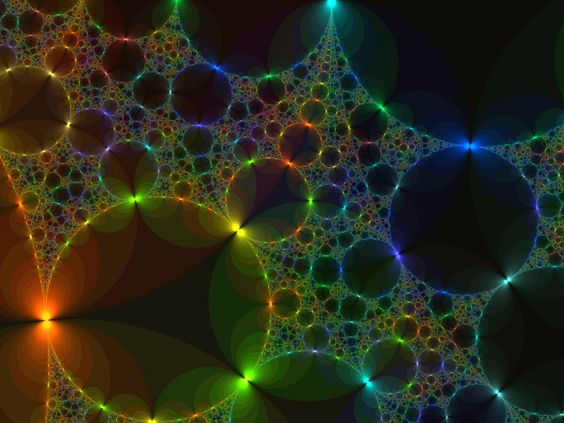
\includegraphics[scale=0.3]{imagenes/burbujas.jpg}
    } \hspace{0.5cm}
    \subfigure[El mundo, dividido en Diagramas de Voronoi, en base a las capitales más cercanas.]{
        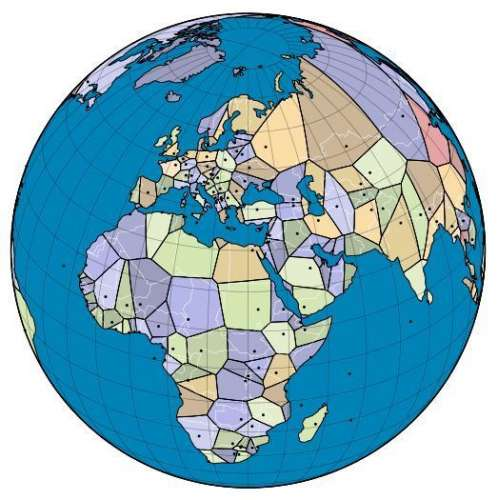
\includegraphics[scale=0.3]{imagenes/mundo.jpg}
    }
    \subfigure[Podemos encontrarlos en la naturaleza.]{
        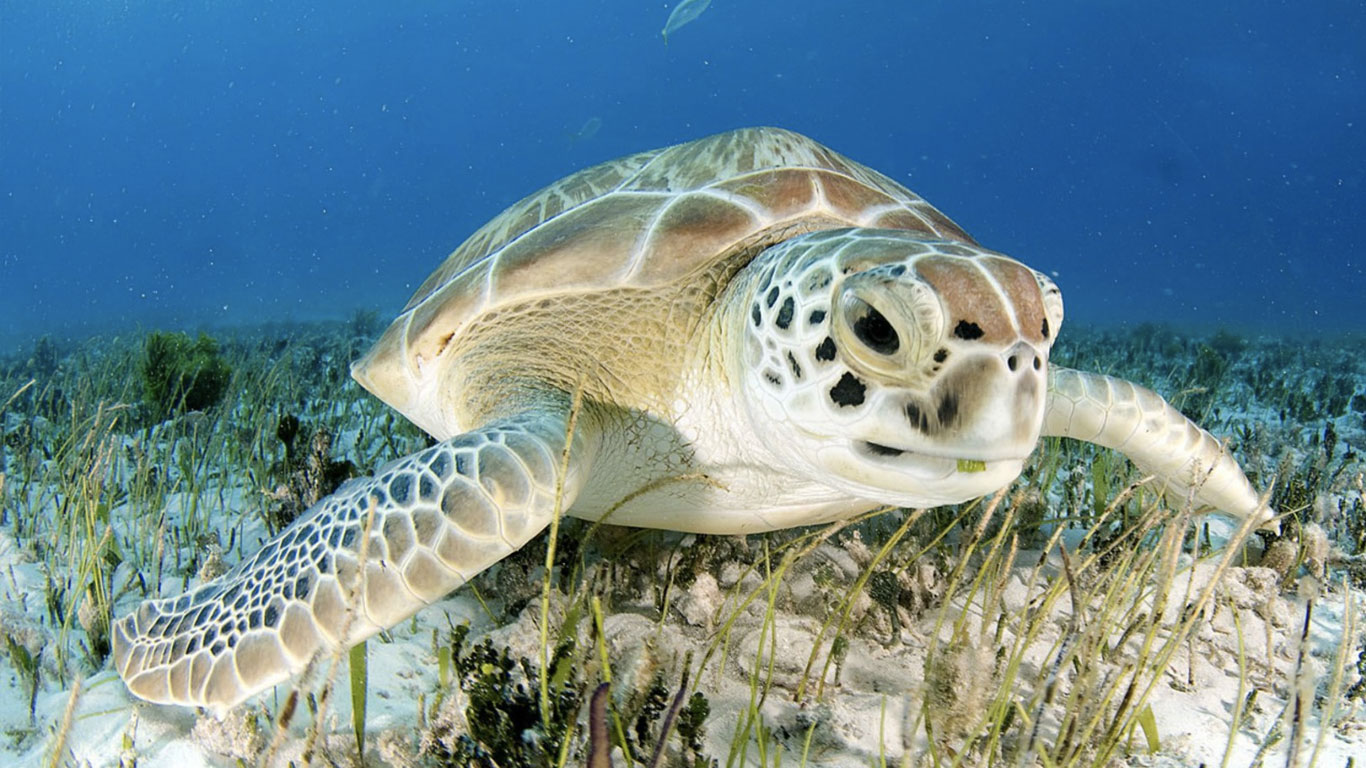
\includegraphics[scale=0.1]{imagenes/tortuga.jpg}
        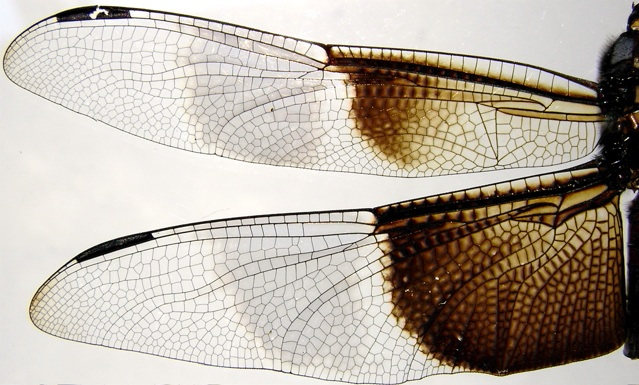
\includegraphics[scale=0.2]{imagenes/alas.jpg}
        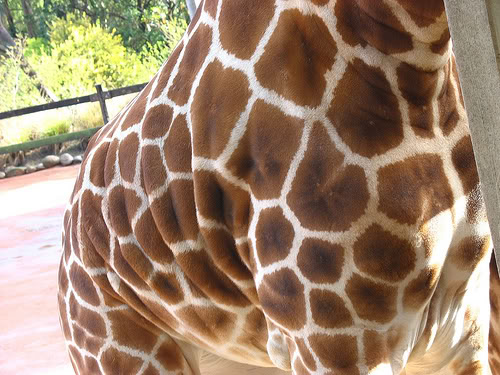
\includegraphics[scale=0.2]{imagenes/jirafa.jpg}
        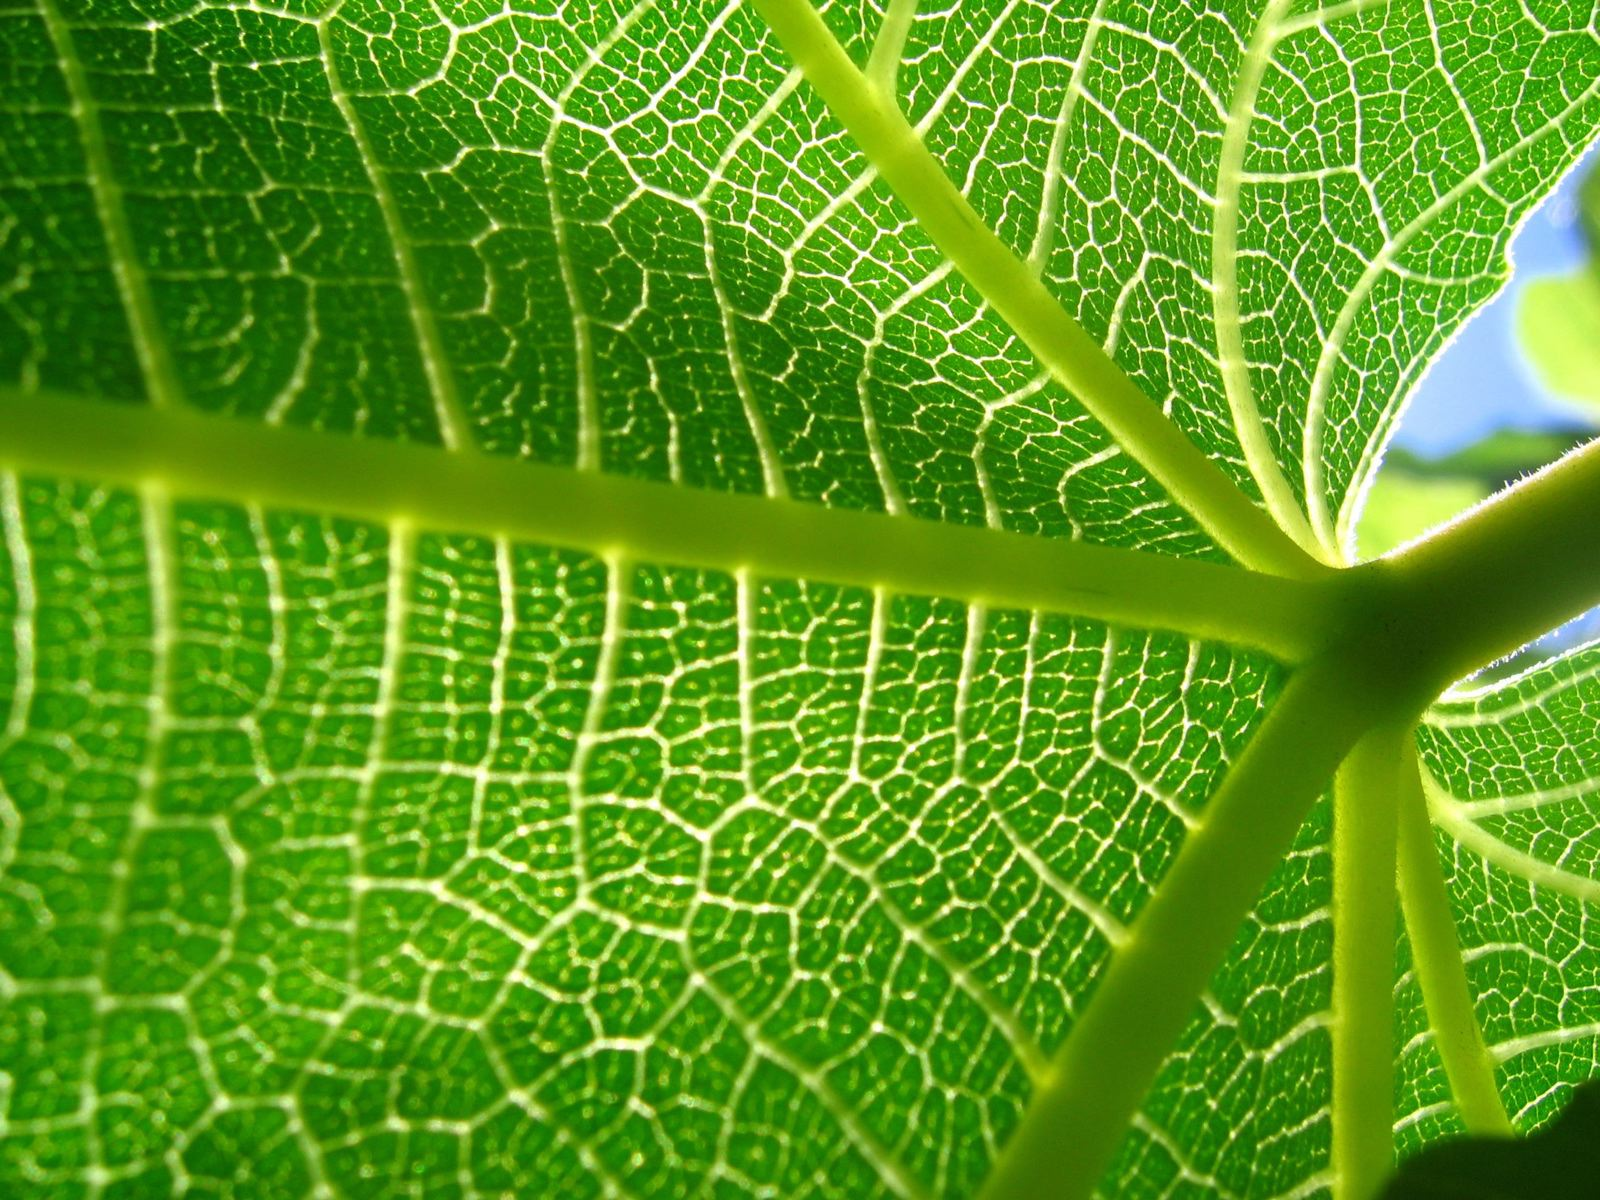
\includegraphics[scale=0.15]{imagenes/hoja.jpg}
    } \hspace{0.5cm}
     \subfigure[Mapa político de España, cuyos puntos son las provincias y las aristas las comunidades autónomas.]{
        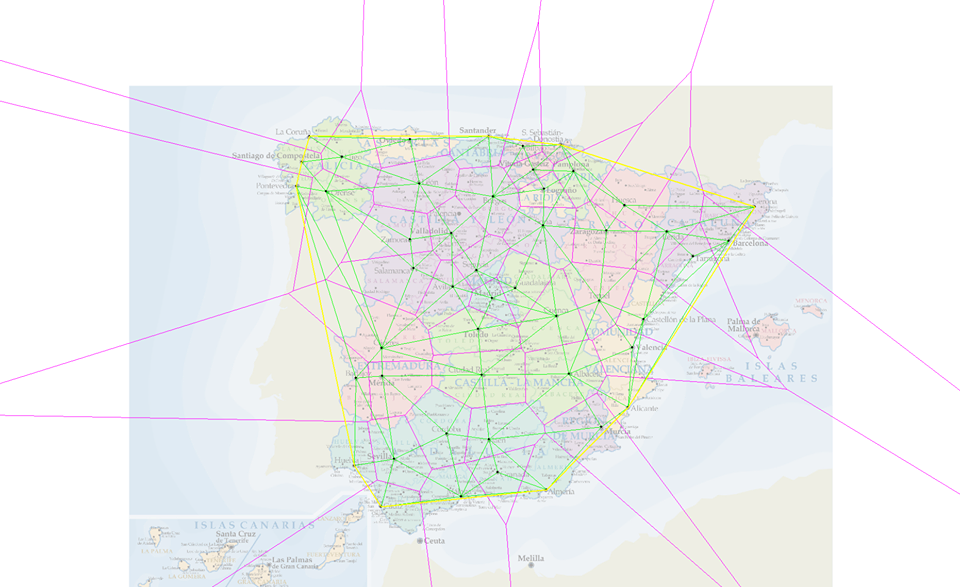
\includegraphics[scale=0.2]{imagenes/capitales.png}
    }
    \subfigure[Edificio Airespace en Tokyo.]{
        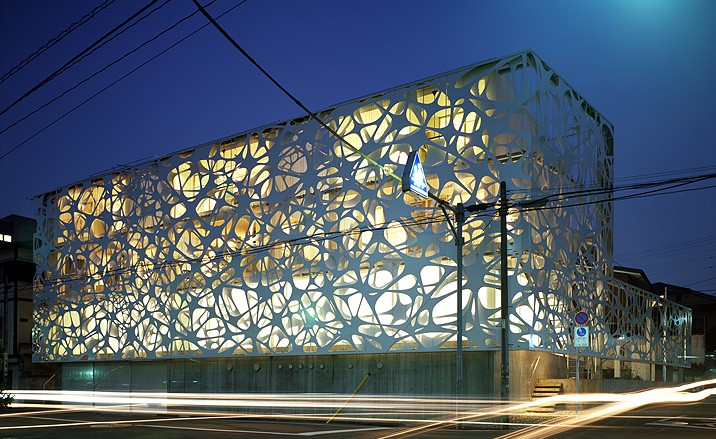
\includegraphics[scale=0.2]{imagenes/airspace.jpg}
    }   
    \caption{Curiosidades de los Diagramas de Voronoi.} \label{fig:incre}
\end{figure}

\begin{comment} ---------------CAPÍTULO 4--------------- \end{comment}

\chapter{Triangulación de Delaunay}$\label{capi4}$

En este capítulo consideramos una estructura muy relacionada con los Diagramas de Voronoi que tiene una relevancia importante en el campo de la geometría computacional, especialmente en gráficos 3D por computadora. Se trata de una red de triángulos conexa y convexa que cumple la condición de Delaunay. Hablaremos de algunas propiedades importantes que posee y concluiremos hablando del grafo del vecino más cercano, que es un subgrafo de las aristas de la Triangulación de Delaunay. 

Este concepto dual, también tiene una historia marcada por redescubrimientos, aunque no tan frecuentes como el caso de los Diagramas de Voronoi. Aunque fue Delaunay quien definió la Teselación (mosaico) usando el método de la esfera vacía, la idea se originó con Voronoi en 1908, que la definió por medio de relaciones entre vecinos, refiriéndose a la estructura resultante como el ensamble de símplices (envolventes convexas). Una de las propiedades importantes de la Teselación de Delaunay en dos dimensiones es que los triángulos individuales son tan equiláteros como sea posible.
Dicha triangulación ha sido ampliamente estudiada en el ámbito de la geometría computacional debido a sus aplicaciones en diferentes áreas de la ciencia y la ingeniería. Nos va a ser muy útil para la construcción del Diagrama de Voronoi ya que antes de dibujar cualquier región de Voronoi, primero trazaremos su respectiva Triangulación de Delaunay en la que nos apoyaremos marcando el punto central de cada circunferencia y trazando perpendiculares a las aristas de los triángulos. 

\begin{comment} --------------- 3.1 -------------- \end{comment}

\section{Formalización}

La Triangulación de Delaunay (Borís Nikolaevich Delaunay, 1934), $DT(S)$, es el dual del Diagrama de Voronoi con todos sus circuncentros: la circunferencia circunscrita de un triángulo es la circunferencia que contiene los tres vértices del triángulo.
Luego, los circuncentros que quedan tras hacer la Triangulación de Delaunay son los vértices de los segmentos del Diagrama de Voronoi. La unión de estos circuncentros produce el Diagrama de Voronoi, tal y como podemos ver en las siguientes figuras:

 \begin{figure}[H]
    \subfigure[Triangulación con todas las circunferencias circunscritas y sus centros.]{ 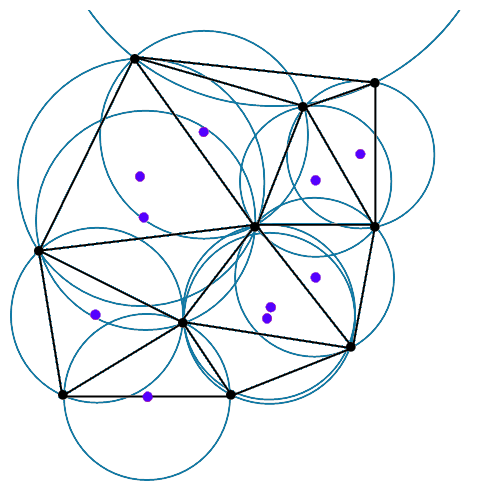
\includegraphics[scale=0.5]{imagenes/delaunay_circumcircles_centers.png}} \hspace{1cm}
    \subfigure[Diagrama de Voronoi obtenido uniendo los centros de las circunferencias circunscritas.]{
    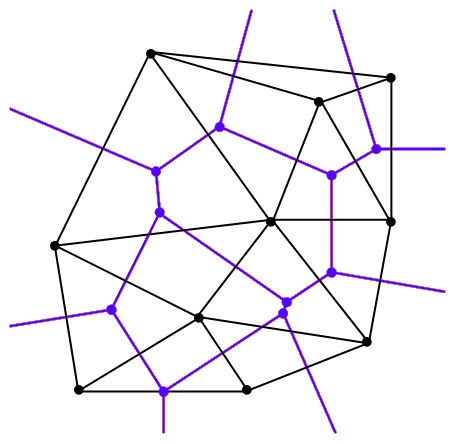
\includegraphics[scale=0.5]{imagenes/delaunay_voronoi.png}}
    \caption{La unión de los circuncentros de la Triangulación de Delaunay produce el Diagrama de Voronoi.}\label{fig:tri}
\end{figure}


\begin{definicion} La \textbf{triangulación} (o red triangular), $T$, de $\mathcal{S}$ es un conjunto máximo de segmentos de línea no cruzados por los sitios en $\mathcal{S}$. En otras palabras, $T$ define una partición de la envolvente convexa de $\mathcal{S}$ en triángulos cuyo conjunto de vértices es exactamente $\mathcal{S}$. \end{definicion} 


El número de diferentes particiones de este tipo es grande (de hecho, exponencial) para cada conjunto de puntos de $n \in \mathcal{S}$ en posición general, lo que hace que los resultados de optimalidad sean aún más valiosos.
Diremos, además, que: \begin{definicion} $T$ es \textbf{localmente Delaunay} si, para cada uno de sus cuadriláteros convertidos, $Q$, los correspondientes dos triángulos (adyacentes) tienen circunferencias vacías de vértices de $Q$. \end{definicion}
Claramente, $DT(S)$ es localmente Delaunay porque las circunferencias para sus triángulos están totalmente vacías de sitios (ver Teorema $\ref{th31})$. Curiosamente, la propiedad local también implica la global.

La Triangulación de Delaunay es una de las triangulaciones más interesantes por ser aplicable para la resolución de multitud de problemas aparentemente sin relación entre sí, debido a sus propiedades geométricas, y por contar con algoritmos bastante eficientes para su cálculo. Además, tiene una serie de propiedades que detallaremos a continuación y hacen que este diagrama pueda servir para conocer el área de influencia de cada punto, encontrar el lugar del plano más alejado de los puntos que actualmente forman la nube, encontrar el punto más cercano a un lugar del plano cualquiera, averiguar dónde situar un punto para que su área de influencia sea mayor teniendo en cuenta los puntos ya existentes en el plano... Con todas estas características, podemos darnos cuenta de por qué las aplicaciones (\ref{aplicaciones}) en la vida real de este diagrama son incontables y sobre campos muy diferentes.\vspace{0.3cm}

De manera más formal, diremos que una red de triángulos es una \textbf{Triangulación de Delaunay} si todas las circunferencias circunscritas de todos los triángulos de la red son vacías, es decir, no contienen otros vértices aparte de los tres que la definen (condición de Delaunay). Esto es, no debe contener ningún vértice de otro triángulo (definición original para espacios bidimensionales). Si esta definición queremos ampliarla para espacios tridimensionales (para dimensiones más grandes se puede hacer pero no se usa en la práctica), podemos hacerlo usando la esfera circunscrita. Esta condición nos asegura que los ángulos del interior de los triángulos son lo más grandes posibles, por lo que maximiza la extensión del ángulo más pequeño de la red. Además, la triangulación forma la envolvente convexa del conjunto de puntos y es unívoca si no hay más de tres vértices en ningún borde de la circunferencia circunscrita. Esto es muy práctico porque los errores de redondeo son mínimos y es por ésto que las triangulaciones de Delaunay se utilizan en aplicaciones gráficas.
\vspace{0.3cm}

Las siguientes figuras muestran que si queremos construir una triangulación a partir de algunos puntos, es fácil hacerlo simplemente conectando los vértices. Además, con la condición de Delaunay, podemos estudiar si la triangulación a realizar es útil.

\begin{figure}[H]
    \subfigure[De algunos puntos requerimos construir una triangulación.]{ 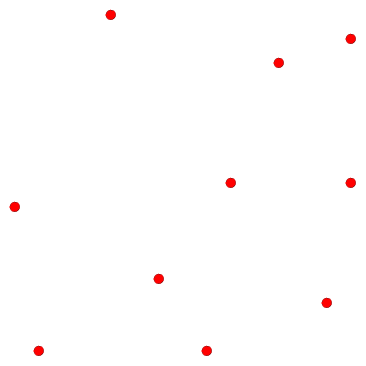
\includegraphics[scale=0.4]{imagenes/delaunay_points.png}}
    \subfigure[Conectando los vértices podemos obtener cualquier triangulación.]{
    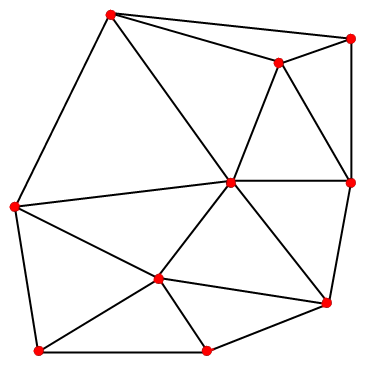
\includegraphics[scale=0.4]{imagenes/delaunay_small.png}}
    \subfigure[Con la condición de Delaunay podemos examinar si la triangulación es útil.]{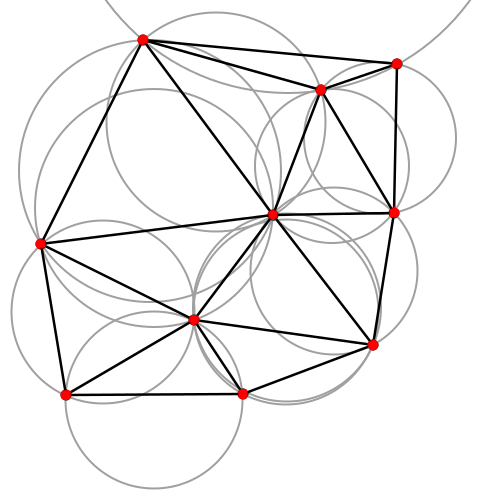
\includegraphics[scale=0.25]{imagenes/delaunay_circumcircles.png}}
    \caption{Triangulación de Delaunay de 10 puntos en el plano, mostrando la circunferencia de cada triángulo.} \label{fig:tri}
\end{figure} 

\section{Propiedades}$\label{propDT}$
Una vez conocido el Diagrama de Voronoi, pueden definirse una serie de propiedades que permiten calcular una Triangulación de Delaunay a partir de dicho diagrama de forma directa e inequívoca. Es por eso que se dice que el Diagrama de Voronoi y la Triangulación de Delaunay son duales.  
\vspace{0.3cm}

Cada triangulación de $\mathcal{S}$ contiene las aristas de la envolvente convexa de $\mathcal{S}$ y sus caras acotadas son triángulos. Su número, como ya vimos, es exactamente igual a \textit{2n - h - 2}, donde \textit{h} representa los vértices de la envolvente convexa. El número de aristas es \textit{3n - h - 3}. Obsérvese que ambos números, que se derivan fácilmente de la fórmula de poliedro de Euler, son independientes de la forma de triangular el conjunto de puntos $\mathcal{S}$, por las características de esta fórmula. 
\vspace{0.3cm}

Llamaremos a un subconjunto conectado de aristas de una triangulación una \textbf{teselación} de $\mathcal{S}$ si contiene las aristas de la envolvente convexa y si cada punto de $\mathcal{S}$ tiene al menos dos aristas incidentes.

La \textbf{teselación de Delaunay}, $DT(S)$, es obtenida conectando con un segmento de línea cualesquiera dos puntos $p, q$ de $\mathcal{S}$ para los cuales existe un círculo que pasa por $p$ y $q$ pero no contiene ningún otro sitio de $\mathcal{S}$ en su interior o límite. Las aristas (o bordes) de $DT(S)$ las llamaremos \textbf{aristas de Delaunay}.

\begin{lema}
	Dos puntos de $\mathcal{S}$ están conectados por una arista de Delaunay si y sólo si sus regiones de Voronoi tienen una arista adyacente.
\end{lema}

Dos regiones de Voronoi pueden compartir, al menos, una arista de Voronoi, por convexidad. Además, este lema implica que $DT(S)$ es el grafo teórico dual de $V(S)$ creado mediante aristas rectas. De forma biyectiva, las aristas de Delaunay se corresponden con las aristas de Voronoi; las caras de Delaunay serán los vértices de Voronoi; y los vértices de Delaunay serán las regiones de Voronoi.

\begin{teorema}\label{th31}
    Si el conjunto de puntos $\mathcal{S}$ está en posición general (no hay cuatro puntos coplanares, no hay cinco puntos co-esféricos), entonces $DT(S)$, el dual del Diagrama de Voronoi $V(S)$, es una triangulación de $\mathcal{S}$, llamada Triangulación de Delaunay. Tres puntos de $\mathcal{S}$ dan como resultado exactamente un triángulo de Delaunay si el círculo que definen no contiene ningún otro punto de $\mathcal{S}$.
\end{teorema}

La Triangulación de Delaunay posee varias características acerca de sus propiedades de optimización, sus estructuras como subgrafos y su flexibilidad para adaptarse a dimensiones más altas. Contiene un tetraedro para cada vértice, un triángulo para cada arista y una arista para cada cara de $V(S)$. Equivalentemente, $DT(S)$ puede definirse usando la propiedad de esfera vacía, declarando un tetraedro extendido por $S$ como Delaunay si su circunferencia está vacía de sitios en $\mathcal{S}$. Los centros de estas esferas vacías son sólo los vértices de $V(S)$.
$DT(S)$ es una partición de la envolvente convexa de $\mathcal{S}$ en tetraedros, siempre que $\mathcal{S}$ esté en posición general. Obsérvese que, para configuraciones especiales de puntos en el espacio de tres dimensiones, las aristas de $DT(S)$ ya pueden formar el grafo completo en $\mathcal{S}$, es decir, el grafo donde todos los pares de vértices ${n \choose 2}$ coinciden con un borde. El conjunto de celdas $DT(S)$ es llamado la \textbf{tetraedrización de Delaunay} para $\mathcal{S}$.

\subsection{Propiedades de optimización}

Veamos ahora algunas características avanzadas del diagrama dual de Voronoi.
\vspace{0.3cm}

La Triangulación de Delaunay, $DT(S)$, de un conjunto $\mathcal{S}$ de $n$ sitios en el plano posee una serie de propiedades agradables y útiles, muchas de las cuales son bien conocidas y comprendidas hoy en día. Al ser el dual geométrico del Diagrama de Voronoi $V(S)$, $DT(S)$ comprende la información de proximidad inherente a $\mathcal{S}$ de una manera compacta. Aquí nos fijamos en $DT(S)$ como una triangulación por sí misma y nos concentramos en los parámetros que son optimizados por $DT(S)$ sobre todas las posibles triangulaciones del punto establecido de $\mathcal{S}$. Debemos tener en cuenta la definición más teórica de triangulación:

\vspace{0.3cm}

\begin{teorema}$\label{th32}$
    Una triangulación de $\mathcal{S}$ es localmente Delaunay si y sólo si es igual a la Triangulación de Delaunay, $DT(S)$.
\end{teorema}

\begin{proof}
    Sea $T$ una triangulación de $\mathcal{S}$ y supongamos que $T$ es localmente Delaunay. Se muestra que, para cada triángulo $\bigtriangleup$ de $T$, su circunferencia $C(\bigtriangleup)$ está vacía de sitios en $\mathcal{S}$.
    
    Asumiendo el contrario, dejemos $s$ dentro de $C(\bigtriangleup$) para algunos $s \in{\mathcal{S}}$ y algunos $\bigtriangleup$ en $T$. Observamos que $s \notin{\mathcal{S}}$ y sea $e$ la arista de $\bigtriangleup$ más cercana a $s$. Supongamos, sin pérdida de generalidad, que $(\bigtriangleup,e,s)$ maximiza el ángulo extendido por $e$ en $s$, para todos los triples (triángulo, arista, sitio).
    
    Debido a $s$, la arista $e$ no puede ser una arista de la envolvente convexa de $\mathcal{S}$. Dejemos que el triángulo $\bigtriangleup'$ sea adyacente a $\bigtriangleup$ en $e$, y sea $s'$ el tercer vértice de $\bigtriangleup'$. Como $T$ es localmente Delaunay, $s'$ está fuera de $C(\bigtriangleup$), por lo tanto $s \neq s'$. Ahora, observamos que $s$ está encerrado por $C(\bigtriangleup'$), y sea $e'$ la arista de $\bigtriangleup'$ más cercana a $s$. El ángulo en $s$ para ($\bigtriangleup,e',s)$ es mayor que el de ($\bigtriangleup',e,s)$, lo que da una contradicción.
\end{proof}
\vspace{0.3cm}

\begin{definicion}
    Un \textbf{giro de arista} en una triangulación $T$ de $\mathcal{S}$ es el intercambio de las dos diagonales en uno de los cuadriláteros de conversión de $T$. Lo llamaremos \textbf{giro bueno} si, después del giro, la triangulación dentro del cuadrilátero (que consta de sólo 2 triángulos) es localmente Delaunay. El intercambio repetido de diagonales en el mismo cuadrilátero siempre produce una secuencia alternada de buenos malos giros.
\end{definicion}
\vspace{0.3cm}

Por tanto, el anterior teorema $\ref{th32}$ ahora puede usarse para probar que $DT(S)$ optimiza varias medidas de calidad, mostrando que cada buena inversión incrementa la calidad. Cualquier secuencia de buenos giros termina entonces en el óptimo global, la Triangulación de Delaunay. La longitud de una secuencia de este tipo está limitada por ${n \choose 2}$, ya que una arista que se desvía no puede volver a aparecer.
\vspace{0.3cm}

Una de las medidas de calidad más prominentes se refiere a los ángulos que ocurren en una triangulación. Recordemos que el número de aristas (y por tanto de los triángulos) no depende del camino de las triangulaciones $\mathcal{S}$, y sea $t$ el número de triángulos de $\mathcal{S}$. La \textbf{angulosidad} de una triangulación se define como la lista ordenada de ángulos $(\alpha_{1},...,\alpha_{3t})$ de sus triángulos, en orden ascendente. 


\begin{definicion}
    Una triangulación se llama \textbf{equiangular} si posee lexicográficamente la mayor angularidad entre todas las triangulaciones posibles para $\mathcal{S}$. De hecho, cada buen giro aumenta la angularidad. En el caso de cocircularidades entre los sitios, $DT(S)$ no es una triangulación completa, como vimos en las propiedades básicas al comienzo de esta sección $\ref{propDT}$.
\end{definicion}

\begin{teorema}$\label{th33}$
    Sea $\mathcal{S}$ un conjunto finito de sitios en el plano. Una triangulación de $\mathcal{S}$ es equiangular solamente si es una terminación de $DT(S)$.
\end{teorema}


La triangulación equiangular maximiza, obviamente, el ángulo mínimo que ocurre en todos los triángulos. Esta propiedad es deseable para aplicaciones de generación de malla en modelado de terreno o para el método de elementos finitos. Por este teorema $\ref{th33}$, tales triangulaciones pueden ser computadas en tiempo $O(nlog(n))$ con los algoritmos de Triangulación de Delaunay que veremos, más adelante, en el Capítulo $\ref{algoritmos}$.
\vspace{0.3cm}


\subsection{El vecino más cercano}

La Triangulación de Delaunay $DT(S)$ de un conjunto $\mathcal{S}$ de $n$ puntos contiene, como subgrafos, diversas estructuras con diversas aplicaciones (como por ejemplo árboles y ciclos mínimos). 
\vspace{0.3cm} 

Nosotros nos centraremos en uno de los ejemplos más importantes, el \textbf{grafo del vecino más cercano}\label{vecino} de $\mathcal{S}$, problema de distancia que el Diagrama de Voronoi resuelve directamente: para cada punto del conjunto $\mathcal{S}$, se requiere un vecino más cercano en $\mathcal{S}$. Esto puede responderse construyendo en primer lugar un Diagrama de Voronoi para luego localizar la celda del diagrama que contiene a dicho punto.
La solución ofrecida por este diagrama se basa en el siguiente hecho.

\begin{lema}$\label{lema32}$
    Sea $\mathcal{S}=P\cup Q$ una descomposición disjunta del conjunto de puntos $\mathcal{S}$, y $p_{0} \in P$ y $q_{0} \in Q$ sean tales que: \begin{equation}d(p_{0},q_{0})= \min_{p\in P, q\in Q} d(p,q) \end{equation}
    Entonces, las regiones de Voronoi de $p$ y $q$ son adyacentes a la arista en $V(S)$.
\end{lema}
\begin{proof}
    En caso contrario, el segmento de línea $p_{0}q_{0}$ contiene un punto $z$ que pertenece al cierre de alguna región de Voronoi $VR(r, S)$, donde $r \not= p_{0},q_{0}$. Supongamos que $r$ pertenece a $Q$; El caso $r \in P$ es simétrico. 
    Desde $z \in VR(r,S)$ se sigue que $d(z,r)\leq d(z,q_{0})$, de ahí
    \vspace{0.3cm}
    
    $d(p_{0},r)\leq d(p_{0},z)+d(z,r) \leq d(p_{0},z)+d(z,q_{0})=d(p_{0},q_{0})\leq d(p_{0},r)$
    \vspace{0.3cm}
      
    Por minimalidad de $d(p_{0},q_{0})$. Por lo tanto, la igualdad debe mantenerse, y obtenemos $d(p_{0},r)=d(p_{0},q_{0})$ y $d(z,r)=d(z,q_{0})$.

    Pero como $p_{0}$ está en la bisectriz $B(q_{0},r)$, cada punto $z$ en el interior de $\bar{q_{0}p_{0}}$ es estrictamente cercano a $q_{0}$ que a $r$, luego llegamos a una contradicción.

\end{proof}
\vspace{0.3cm}

Si aplicamos este lema \ref{lema32} a los subconjuntos ${q}$ y $\mathcal{S}\setminus{p}$, se sigue que el vecino más cercano de $p$ está incluido en una región vecina de Voronoi (por ejemplo, es un vecino de Delaunay). Por lo tanto, es suficiente examinar, para cada $p \in \mathcal{S}$, todos los vecinos de $p$ en el Diagrama de Voronoi, y seleccionar el más cercano de ellos. De esta manera, cada arista de $V(S)$ se accede dos veces. Dado que su número total es lineal (ver Lema \ref{lema43}), podemos resolver el problema del vecino más cercano construyendo el Diagrama de Voronoi.

\begin{teorema}
    Dado un conjunto $\mathcal{S}$ de $n$ puntos en el plano, un tiempo $O(nlog(n))$ y espacio lineal son suficientes para determinar, para cada $p \in \mathcal{S}$, un vecino más cercano en $\mathcal{S}$.
\end{teorema}
 
 
Si para cada $p$ su vecino más cercano en $\mathcal{S}$ es conocido, podemos determinar fácilmente un par de puntos cuya distancia es mínima.

\begin{corolario}
    El par más cercano entre $n$  puntos en el plano se puede determinar dentro de un tiempo $O(nlog(n))$ y espacio lineal.
\end{corolario}


El par más cercano en $\mathcal{S}$ corresponde a la arista más corta de la Triangulación de Delaunay $DT(S)$, como lo muestra el Lema \ref{lema32}. El segundo par más cercano, debe estar en $DT(S)$ también, ya que ambas aristas están en el árbol de expansión mínimo de $\mathcal{S}$, que es un subgrafo de $DT(S)$.

\begin{teorema}
    Los $k$ pares más cercanos de un conjunto $\mathcal{S}$ de $n$ puntos se pueden calcular en tiempo $O((n+k)log(n))$ y espacio $O(n+k)$.
\end{teorema}

Aparte de este ejemplo, existen algoritmos eficientes para programar estas estructuras que se siguen del hecho de que $DT(S)$ tiene un tamaño $O(n)$ y pueden ser construidos en tiempo $O(nlog(n))$ en el plano. Este efecto positivo se pierde parcialmente en dimensiones más altas, ya que $DT(S)$ puede ser el grafo completo en $\mathcal{S}$ ya en tres dimensiones. 
\vspace{0.3cm}


Podemos concluir diciendo que las triangulaciones de Delaunay son una herramienta muy útil para generar mallas irregulares a partir de un conjunto de puntos. Existen buenos algoritmos para su cálculo que han sido implementados con éxito. Sin embargo, en general, las implementaciones que se emplean no utilizan la potencia y capacidad de las tarjetas gráficas. Por ejemplo, en el desarrollo de una aplicación informática para emular la evolución de bosques, se calculan Diagramas de Voronoi de forma gráfica como medio de solventar el problema del cálculo de Diagramas de Voronoi generalizados con pesos tanto aditivos como multiplicativos. A continuación, hablaremos de algunas de las posibles estrategias para calcular la Triangulación de Delaunay a partir de un conjunto de puntos de entrada. 

\begin{comment} ---------------CAPÍTULO 5--------------- \end{comment}

\chapter{Algoritmos para el cálculo de Diagramas de Voronoi}\label{algoritmos}

Este capítulo se encuentra a caballo entre la geometría y la computación. Explicaremos, de manera más teórica, algunos de los algoritmos más conocidos y utilizados para la implementación de los Diagramas de Voronoi. Estos algoritmos nos serán muy útiles en el desarrollo y realización de la librería para su cálculo y gestión, que veremos en el siguiente capítulo $\ref{capi6}$.
\vspace{0.3cm}

El Diagrama de Voronoi, $V(S)$, y la Triangulación de Delaunay, $DT(S)$, muestran la influencia de proximidad que $\mathcal{S}$ ejerce de una manera simple e intuitiva, con una descripción de tamaño lineal solamente. Ya hemos revelado en los Capítulos $\ref{capi3}$ y $\ref{capi4}$ el potencial intrínseco oculto que poseen. Ahora, mostraremos que se prestan a varios métodos eficientes de construcción.
\vspace{0.3cm}

Conviene recordar la definición $\ref{orden}$ que nos será útil para entender a qué nos referimos cuando hablamos de complejidad o tiempo empleado en los distintos algoritmos. Veremos distintas maneras de computar una representación geométrica del Diagrama de Voronoi y su dual. Por simplicidad, vamos a asumir que, de los $n$ puntos de $\mathcal{S}$, no hay cuatro de ellos que sean cocirculares y no hay tres que sea colineales. Como vimos en el Teorema $\ref{th31}$, podemos referirnos a DT(S) como la Triangulación de Delaunay. Todos los algoritmos que presentaremos pueden funcionar sin esta suposición de posición general. Además, pueden ser generalizados para otras métricas distintas a la euclídea y a otros lugares que no sean puntos. 
\vspace{0.3cm}

Cualquiera de las dos estructuras permite desplazar eficientemente los bordes incidentes a un vértice dado, o bordeando una cara dada. La estructura de cuatro bordes ofrece la ventaja adicional de describir, al mismo tiempo, un gráfico plano y su dual, de modo que puede usarse para construir tanto el Diagrama de Voronoi como la triangulación de Delaunay. De la DCEL (Double Connected Edge List) de $V(S)$ podemos derivar el conjunto de triángulos que constituyen la Triangulación de Delaunay en tiempo lineal. Por el contrario, del conjunto de todos los triángulos de Delaunay el DCEL del Diagrama de Voronoi se puede construir en el tiempo $O(n)$. Por lo tanto, cada algoritmo para calcular una de las dos estructuras se puede utilizar para calcular el otro, dentro de un esfuerzo $O(n)$ de tiempo extremo.

\vspace{0.3cm}

En cada estructura, un registro está asociado con cada borde $e$ que almacena la siguiente información: los nombres de los dos extremos de $e$; referencias a los bordes en el sentido de las agujas del reloj o en sentido contrario a las agujas del reloj junto a $e$ alrededor de sus extremos; finalmente, los nombres de las caras a la izquierda y a la derecha de $e$. La necesidad de espacio de ambas estructuras es $O(n)$.

\section{Algoritmo de Fuerza Bruta}

Este algoritmo es el más simple posible y consiste en explotar la geometría de cada región de Voronoi y es una primera aproximación para la construcción del Diagrama de Voronoi. Mediante el cálculo explícito de los $n-1$ semiplanos originados debido a los bisectores trazados con respecto a los demás sitios, se construye su región de Voronoi para cada lugar. A continuación, se computa la intersección de estos $n-1$ semiplanos para dar origen a la región de Voronoi. Es decir, consiste en probar todas las opciones posibles.
\vspace{0.3cm}

Este algoritmo tiene muchas desventajas debido al cálculo explícito de los semi-planos. Además, su intersección puede provocar problemas de
precisión en la computadora que pueden ser generados por una versión incorrecta del Diagrama de Voronoi $V(S)$. Por otro lado, no podemos obtener información inmediata de los vecinos de cada sitio que se pueda aprovechar. Dado que se trata de un algoritmo ineficiente, también su complejidad computacional es bastante alta ya que está en el orden de $O(n^2log(n))$.
\vspace{0.3cm}

En las siguientes secciones describimos varios algoritmos que calculan todo el Diagrama de Voronoi dentro de este tiempo. Estos algoritmos son (asintóticamente) los peores casos óptimos.


\section{Algoritmo Incremental}\label{incremental}

Este algoritmo se basa, de manera general, en, supuesto construido el diagrama para $k$ puntos, construir el diagrama para $k+1$. Emplea un tiempo de $O(n)$ en la inserción de cada nuevo punto, con una complejidad total de $O(n^2)$ ya que la región de $p$ puede tener hasta $n-1$ aristas, para $n = |S|$ (donde $| |$ indica la cardinalidad, es decir, el número de elementos en el conjunto). A pesar de su complejidad cuadrática, este ha sido el método más popular y utilizado para construir el Diagrama de Voronoi.
\vspace{0.3cm}

Básicamente, la idea es que la secuencia cíclica de aristas de la nueva región de Voronoi $VR(p,S)$ tiene que ser construida y las partes invalidadas del diagrama $V(S$\textbackslash${p})$ que estén dentro de $VR(p,S)$, borradas.
\vspace{0.3cm}

Suponemos tener un Diagrama de Voronoi $V(S)$ para $n$ sitios y queremos construir el diagrama $V(S')$ después de agregar un sitio $s$. Además, suponemos que $s$ pertenece a uno de los círculos asociados con más de un vértice de Voronoi teniendo en cuenta que no pueden ser vértices de $V(S')$ ya que no se cumpliría la condición de Delaunay.


Sea $V(S_{k})$ el Diagrama de Voronoi para los $k$ primeros sitios $s_{1}, s_{2}, ..., s_{k}$, el algoritmo comienza con $V(S_{k})$ cuando $k=2$ o $k=3$ sitios y se modifica incrementalmente agregando los sitios uno a uno. La idea del algoritmo (\cite{fotosincremental}) es convertir $V(S_{k}-1)$ a $V(S_{k})$ para cada nuevo sitio $s_{k}$ que se agregue. 

Por tanto, el algoritmo (pseudocódigo) es el siguiente: 
    Supóngase construido $V(S_{k}-1)$ y que se agrega un nuevo sitio $s_{k}$:
    \begin{itemize}
        \item Encontrar el sitio $s_{i}$ cuya celda de Voronoi contenga a $s_{k}$.
        \item Dibujar la mediatriz entre $s_{i}$ y $s_{k}$.
        \item La mediatriz cruza la frontera de $V(S_{i})$ en dos puntos: $x_{1}$ y $x_{2}$, entrando en la región de Voronoi adyacente.
        \item Encontrar el punto en el que la bisectriz cruza el límite de la región de Voronoi adyacente.
        \item Encontrar la secuencia de segmentos perpendiculares de los sitios vecinos hasta llegar al punto de partida.
    \end{itemize}


\vspace{0.3cm}
    
Veámoslo gráficamente para entender de manera visual lo siguiente:

\begin{figure}[H]
    \subfigure[Dibujamos la mediatriz entre $s_{i}$ y $s_{p}$.]{ 
        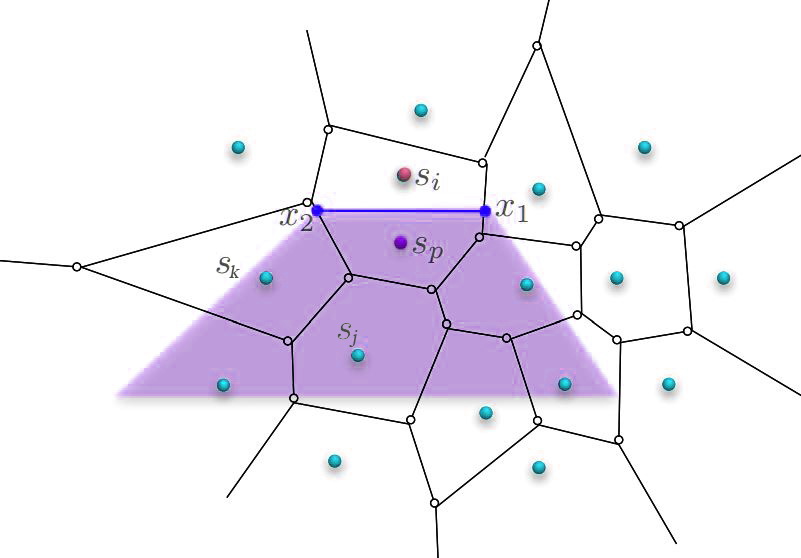
\includegraphics[scale=0.3]{imagenes/incre1.JPG}
    } \hspace{0.5cm}
    \subfigure[Encontramos la secuencia de segmentos perpendiculares hasta llegar al punto de partida.]{
        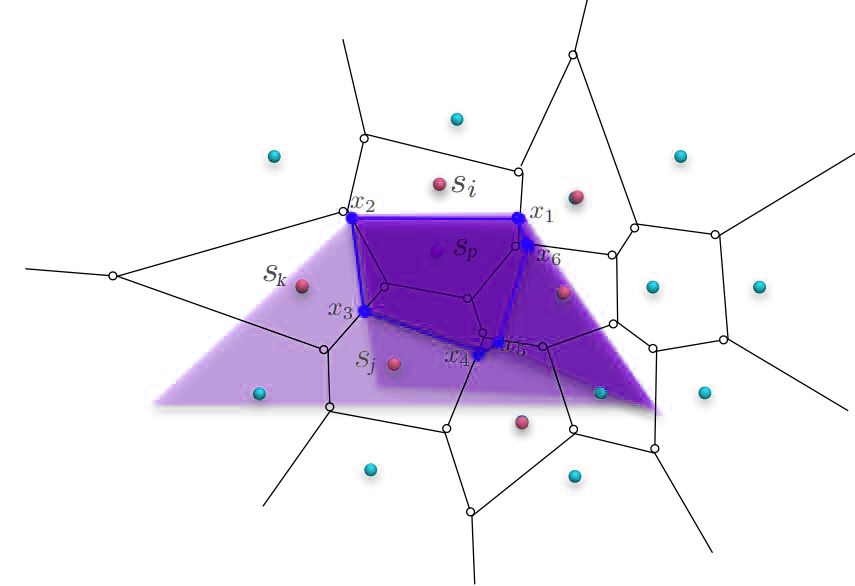
\includegraphics[scale=0.3]{imagenes/incre2.JPG}
    } \hspace{0.5cm}
    \subfigure[Obtención de la región de Voronoi.]{
        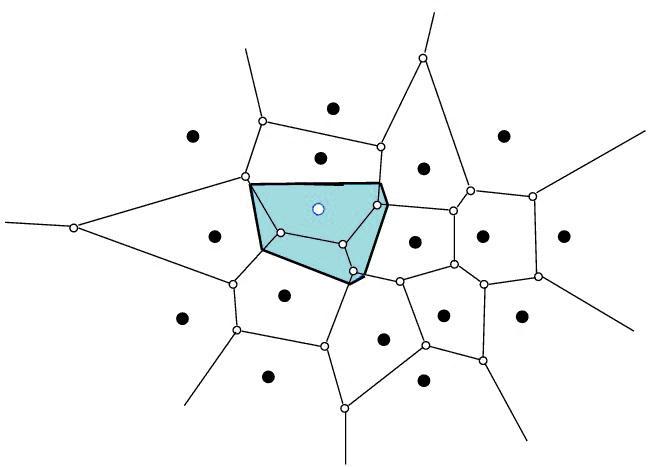
\includegraphics[scale=0.4]{imagenes/incre3.jpg}
    }\hspace{0.5cm}
    \subfigure[Nuevo Diagrama de Voronoi $V(S')$.]{
        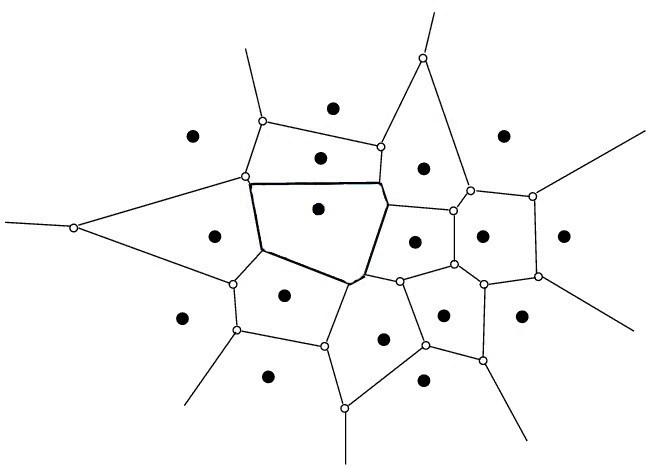
\includegraphics[scale=0.4]{imagenes/incre4.jpg}
    }
    
    \caption{Método Incremental del Diagrama de Voronoi. } \label{fig:incre}
\end{figure}


El sitio $s_{p}$ está a la izquierda del segmento dirigido $x_{1}x_{2}$.
Dicho segmento $x_{1}x_{2}$ divide a la celda convexa en dos partes: la de la izquierda pertenece a la nueva celda $V(S_{p})$ y, además, la mediatriz $\bar{x_{1}x_{2}}$ es una arista de la frontera del nuevo polígono $V(S_{p})$. Entonces, para encontrar el punto de intersección $x_{3}$ habría que trazar la mediatriz $\bar{s_{p},s_{j}}$ hasta unirla con la frontera de $V(S_{j})$. Por tanto, la nueva arista de la región sería el segmento $\bar{x_{2}x_{3}}$.
\vspace{0.3cm}

De manera similar encontramos la secuencia de segmentos de mediatrices de $s_{p}$ y sus sitios vecinos hasta llegar al punto de intersección inicial $x_{1}$.
La secuencia ${x_{1}x_{2}, x_{2}x_{3}, ... , x_{m-1}x_{m}, x_{m}x_{1}}$ es la frontera en orden contrario a las manecillas del reloj de la celda de Voronoi del nuevo sitio $s_{p}$, $V(S_{p})$.
Finalmente, borramos de $V(S)$ la estructura que queda dentro del nuevo polígono $V(S_{p})$ para obtener $V(S’)$. 
\vspace{0.3cm}

La inserción incremental funciona bien en el caso de dimensiones superiores y también para ciertos tipos de Diagramas de Voronoi generalizados y sus duales. Una técnica similar a la inserción incremental es la búsqueda incremental. Se inicia con un solo trazo de Delaunay y luego descubre nuevos, de manera incremental, creando triángulos a partir de bordes de triángulos previamente descubiertos.

\section{Algoritmo de Bowyer-Watson}

Este algoritmo es conocido a veces como el Algoritmo de Bowyer o el Algoritmo de Watson ya que Adrian Bowyer y David Watson lo idearon independientemente uno del otro al mismo tiempo, y cada uno publicó un papel en la misma edición del \textit{"The Computer Journal"} .
\vspace{0.3cm}

En la geometría computacional, el algoritmo de Bowyer-Watson es un método para calcular la Triangulación de Delaunay de un conjunto finito de puntos en cualquier número de dimensiones aunque también puede usarse para obtener un Diagrama de Voronoi de los puntos. Es un algoritmo incremental que funciona agregando puntos, uno cada vez, a una Triangulación de Delaunay válida de un subconjunto de los puntos deseados. Después de cada inserción, se suprimen los triángulos cuyas circunferencias contienen el nuevo punto, dejando un agujero poligonal en forma de estrella que se vuelve triangular con el nuevo punto. Al utilizar la conectividad de la triangulación para localizar los triángulos a eliminar de manera eficiente, el algoritmo puede tomar operaciones $O(nlog(n))$ para triangular $n$ puntos, aunque existen casos degenerados especiales donde esto llega hasta $O(n^2)$.
\vspace{0.3cm}

La base de este algoritmo se basa en la propiedad del círculo vacío circunscrito. Concretamente, en el hecho de que la circunferencia circunscrita de cada triángulo no puede contener otro nodo de la triangulación. 

El siguiente pseudocódigo describe una implementación básica del algoritmo Bowyer-Watson (\cite{b-w}). La eficiencia se puede mejorar de varias maneras. Por ejemplo, la conectividad triangular puede usarse para localizar los triángulos que contienen el nuevo punto en su circunferencia, sin tener que comprobar todos los triángulos. 

\begin{itemize} 
    \item La función Bowyer-Watson recibe como parámetros las coordenadas de los puntos que definen una triangulación.
    \item Crear un triángulo lo suficientemente grande como para contener completamente todos los puntos de entrada.
    \item Para cada punto de la triangulación, agrega todos los puntos de uno en uno.
    \item Buscar todos los triángulos que ya no son válidos debido a la inserción.
    \item Si el punto está dentro de la circunferencia del triángulo, poner triángulo como inválido.
    \item Elimina los triángulos de la estructura creando un hueco.
    \item Para cada borde en triángulo, si el borde no es compartido por ningún otro triángulo de los inválidos, calcula la frontera del hueco.
    \item Para cada triángulo inválido, eliminarlos de la estructura de datos y eliminar el triángulo de la triangulación.
    \item Para cada arista en polígono se vuelve a triangular el hueco.
    \item Para cada triángulo en triangulación, limpiar los triángulos externos a la lista de vértices.
\end{itemize}
      
      
Veámoslo de manera gráfica: 

\begin{figure}[H]
    \subfigure[Generación de la triangulación inicial trivial e inserción del primer nodo.]{ 
        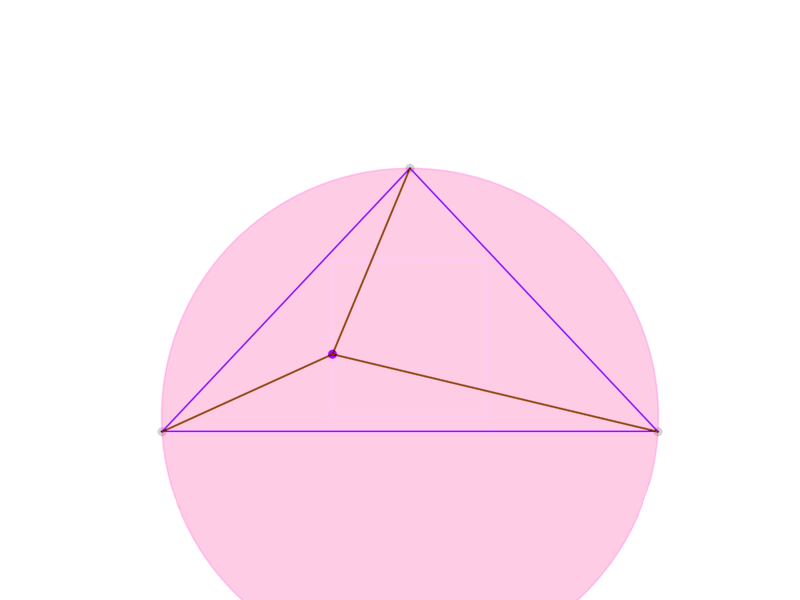
\includegraphics[scale=0.5]{imagenes/Bowyer1.png}
    } \hspace{0.5cm}
    \subfigure[Inserción del segundo nodo.]{
        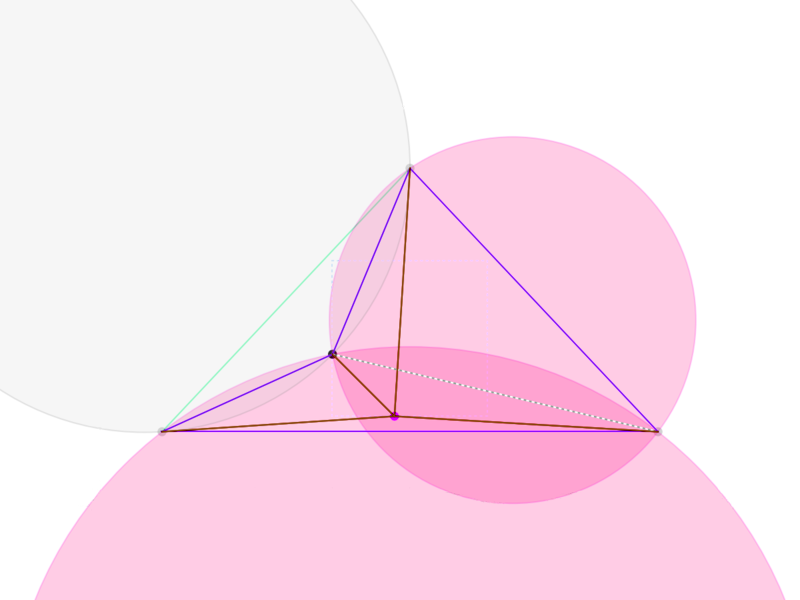
\includegraphics[scale=0.5]{imagenes/Bowyer2.png}
    } \hspace{0.5cm}
    \subfigure[Inserción del tercer nodo.]{
        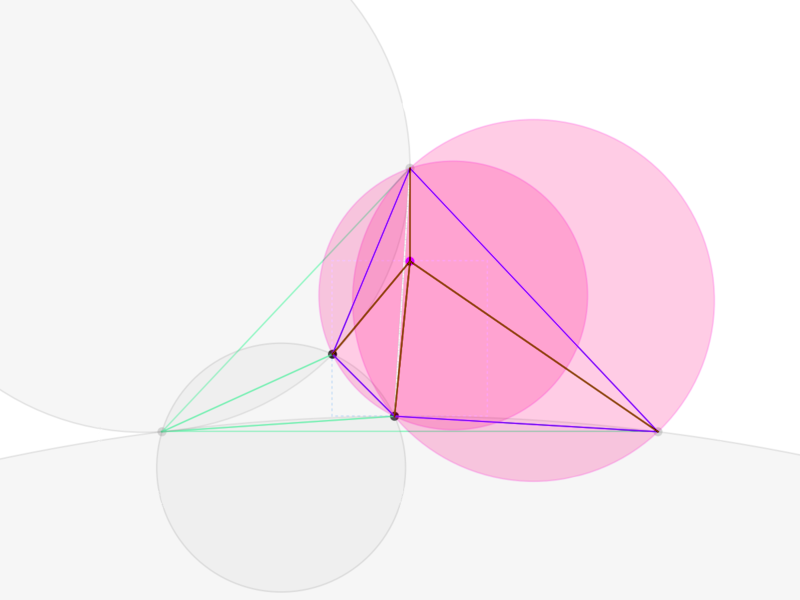
\includegraphics[scale=0.5]{imagenes/Bowyer3.png}
    }\hspace{1.5cm}
    \subfigure[Inserción del cuarto nodo.]{
        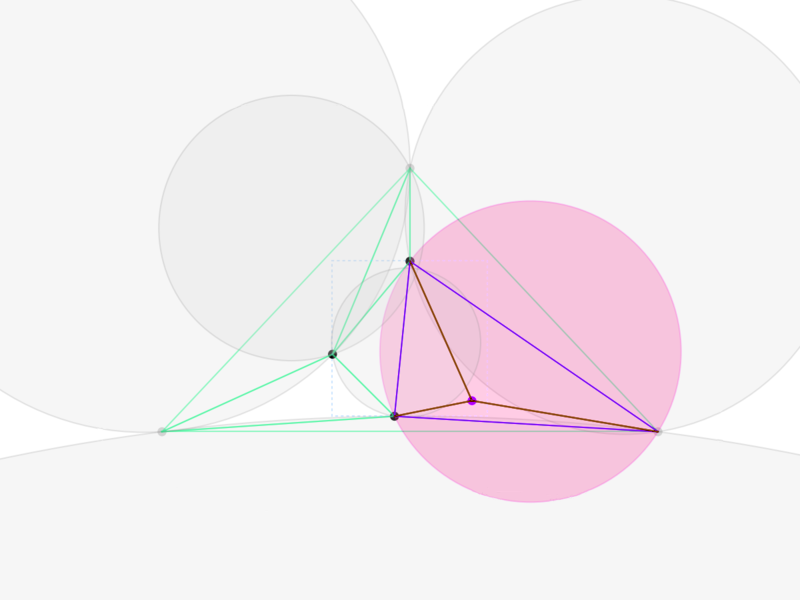
\includegraphics[scale=0.5]{imagenes/Bowyer4.png}
    }\hspace{1.5cm}
    \subfigure[Inserción del quinto nodo.]{
        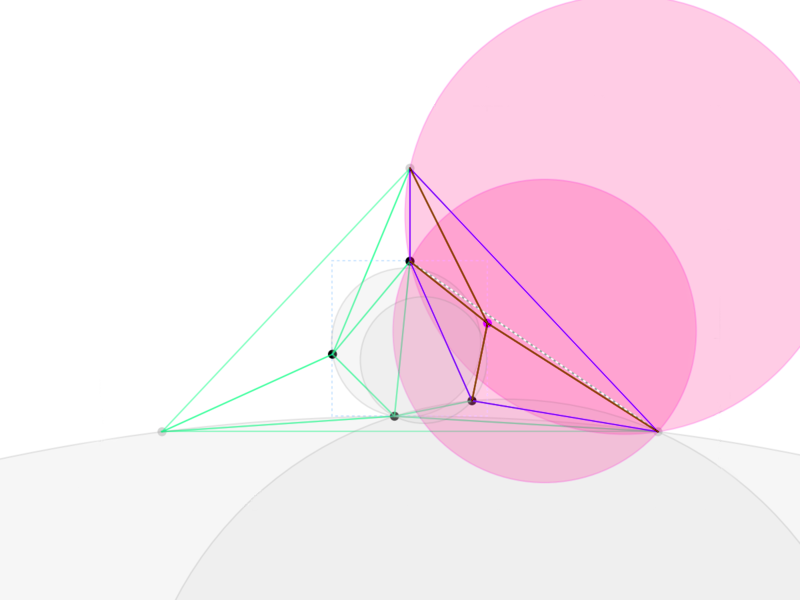
\includegraphics[scale=0.5]{imagenes/Bowyer5.png}
    }\hspace{1.5cm}
    \subfigure[Eliminación de aristas con algún extremo en el super triángulo incial.]{
        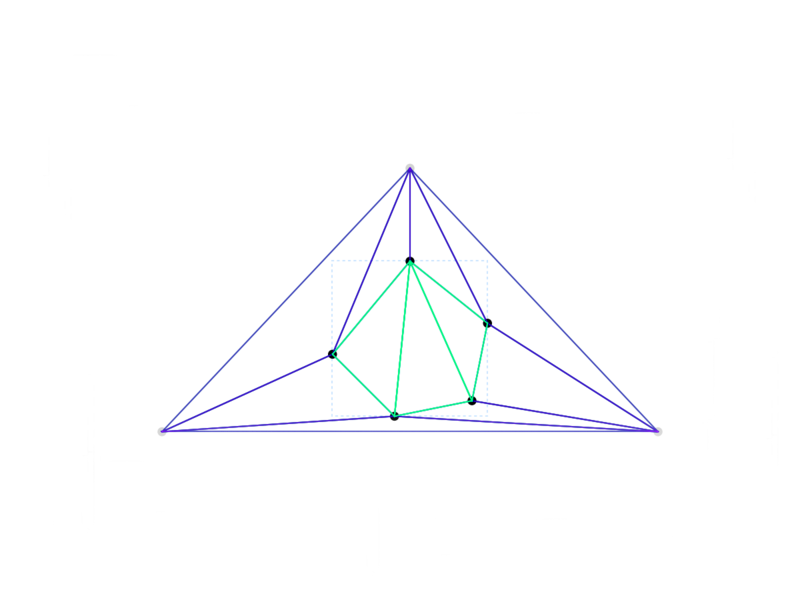
\includegraphics[scale=0.5]{imagenes/Bowyer6.png}
    }
    \caption{Algoritmo Bowyer-Watson.} \label{fig:incre}
\end{figure}

\section{Algoritmo Divide y Vencerás}

Otra manera de construir el Diagrama de Voronoi es con el algoritmo divide y vencerás, que es el algoritmo óptimo del peor caso determinista, en tiempo $O(nlog(n))$. Aunque el algoritmo resulta bastante difícil de implementar, su complejidad es asintóticamente óptima.
\vspace{0.3cm}

El conjunto de puntos de sitios, $\mathcal{S}$, está dividido por una línea en dos subconjuntos $L$ y $R$ de igual tamaño. Entonces, los Diagramas de Voronoi $V(L)$ y $V(R)$ están computados de manera recursiva. Esto es, se aplica la misma estrategia para los conjuntos de puntos (más pequeños) $L$ y $R$. Si sólo dos o tres puntos se dejan en un conjunto, sus diagramas se construyen directamente en un tiempo $O(1)$ (orden constante).
La parte esencial se basa en encontrar la cadena o línea divisoria, es decir, el conjunto de todos los bordes de Voronoi de $V(S)$ que separan regiones de sitios en $L$ de regiones de sitios en $R$, y mezclar $V(L)$ y $V(R)$ para obtener $V(S)$. Durante la recursión, las líneas divisorias, tanto verticales como horizontales, pueden ser fácilmente encontradas si los sitios en $\mathcal{S}$ están ordenados por sus coordenadas $x$ e $y$ de antemano.

Veamos ahora cuáles son los pasos fundamentales de dicho algoritmo de manera gráfica:

\begin{figure}[H]
    \subfigure[Paso 1: Se divide el conjunto en dos mitades de, aproximadamente, el mismo tamaño.]{ 
        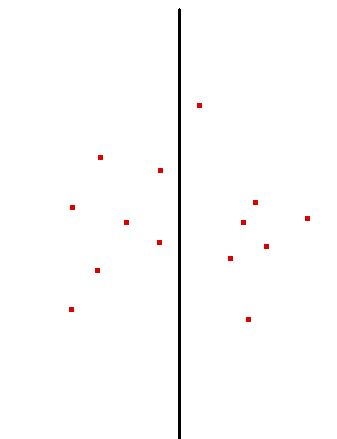
\includegraphics[scale=0.3]{imagenes/paso1.JPG}
    } \hspace{0.5cm}
    \subfigure[Paso 2: Se calcula el Diagrama de Voronoi de la izquierda.]{
        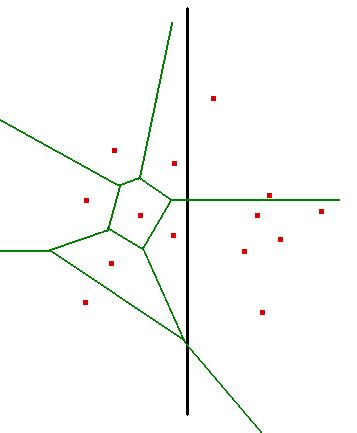
\includegraphics[scale=0.3]{imagenes/paso2.JPG}
    } \hspace{0.5cm}
    \subfigure[Paso 3: Se calcula el Diagrama de Voronoi de la derecha.]{
        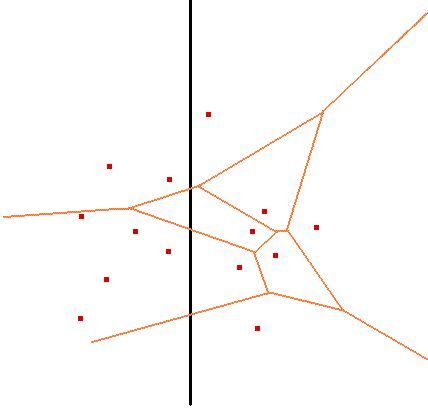
\includegraphics[scale=0.4]{imagenes/paso21.JPG}
    }\hspace{1.5cm}
    \begin{center}
        \subfigure[Paso 4: Se calcula la división.]{
            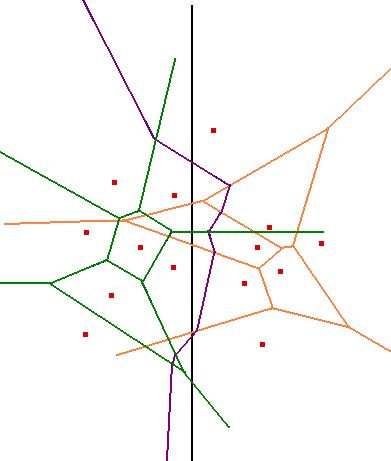
\includegraphics[scale=0.4]{imagenes/paso3.JPG}
        }\hspace{1.5cm}
        \subfigure[Paso 5: Se eliminan todas las líneas de cada diagrama que no caen a su lado de la división.]{
            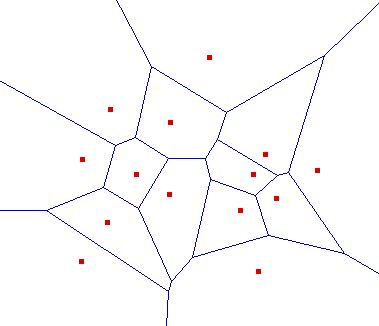
\includegraphics[scale=0.4]{imagenes/paso4.JPG}
        }
    \end{center}
    \caption{Algoritmo Divide y Vencerás. \cite{fotosdividevenceras}} \label{fig:incre}
\end{figure}

Los algoritmos de Divide y Vencerás permiten la paralelización. De hecho, algoritmos eficientes para calcular en paralelo el Diagrama de Voronoi o la Triangulación de Delaunay han sido propuestos por diferentes autores (Blelloch, Edelsbrunner, Shi). Estos autores destacan un algoritmo que utiliza un mapa de levantamiento para $\mathcal{S}$ para construir una cadena de bordes Delaunay que divide $\mathcal{S}$. Demuestran, experimentalmente, que su implementación es comparable en trabajo a los mejores algoritmos secuenciales.
\vspace{0.3cm}

En todo lo referente a este algoritmo, hemos hecho énfasis en que lo complejo está en la fase ascendente (cómo realizar el paso de la fusión). Este paso se complica considerablemente para los Diagramas de Voronoi en un ajuste más general, porque la cadena de fusión puede ciclar e incluso desconectarse.
\vspace{0.3cm}

Una aproximación alternativa, con énfasis en la fase que va desde arriba hacia abajo para realizar el paso de división, se basa en la construcción del eje mediano de una forma general y explota la estructura en árbol de un eje mediano para calibrar la etapa de división.

\section{Algoritmo de Fortune}

Hasta mediados de los ochenta, la mayoría de las implementaciones para computar el Diagrama de Voronoi usaban el algoritmo incremental cuadrático, admitiendo su mayor lentitud para evitar la complejidad del código del algoritmo Divide y Vencerás. En 1985, Fortune inventó un inteligente algoritmo de barrido del plano que resulta tan simple como el incremental, pero en tiempo $O(nlog(n))$ y es capaz, con esta complejidad óptima, de calcular el Diagrama de Voronoi de una nube de puntos en el plano.
Es bastante más complicado que cualquier otro algoritmo de barrido del plano en los que la clave es la capacidad para descubrir todos los eventos próximos de manera eficiente. Por ejemplo, en el algoritmo de barrido del plano para encontrar la intersección de segmentos de línea, éstas son descubiertas antes de que la línea de barrido llegue a ellas (son agregados como eventos futuros).
\vspace{0.3cm}

El problema con el Diagrama de Voronoi es el de predecir cuándo y dónde se producirán los próximos eventos. Imaginemos que detrás de la línea de barrido ya se ha construido el Diagrama de Voronoi basándose en los sitios que se han encontrado hasta ahora en el barrido. La dificultad es que un sitio que queda por delante de la línea de barrido podría generar un vértice de Voronoi que se encuentre detrás de la línea de barrido.
\vspace{0.3cm}

Fortune hizo la inteligente observación de que podía calcularse el Diagrama de Voronoi mediante barrido del plano construyendo una versión “distorsionada” de éste pero que es topológicamente equivalente. Esta versión distorsionada del diagrama se basa en una transformación que modifica la forma en que las distancias son medidas en el plano. El diagrama resultante tiene la misma estructura topológica que el Diagrama de Voronoi, pero sus aristas son arcos parabólicos, en vez de segmentos de línea recta \cite{alfortune}.
\vspace{0.3cm}

En primer lugar, habrá una línea de barrido horizontal, moviéndose de arriba a abajo. También vamos a mantener una curva x-monótona llamada \textbf{línea de playa}. A medida que la línea de barrido se mueve hacia abajo, la línea de playa va justo detrás siguiéndola.
\vspace{0.3cm}

Veamos ahora el mecanismo de barrido de este algoritmo: partimos de un plano de barrido que se mueve de izquierda a derecha sobre el plano $x-y$ con un ángulo de inclinación igual al de los conos.
\vspace{0.3cm}

El plano de barrido intersecta con el plano $x-y$ en lo que hemos llamado línea de barrido. La intersección del plano de barrido con el cono proyectada sobre el plano $x-y$ es una parábola con foco en el punto $p$ y cuya directriz (línea que determina las condiciones de generación de otra línea) es la línea de barrido. Si hacemos opaco el plano de barrido, entonces éste oculta los conos de la derecha de la línea de barrido; los conos visibles que todavía no han sido totalmente barridos por el plano de barrido proyectarán sobre el plano $x-y$ un conjunto de parábolas apuntando hacia la izquierda, con ejes paralelos y distintas anchuras.

\begin{figure}[H]
    \subfigure[Círculos de elevación sobre el cono.]{ 
        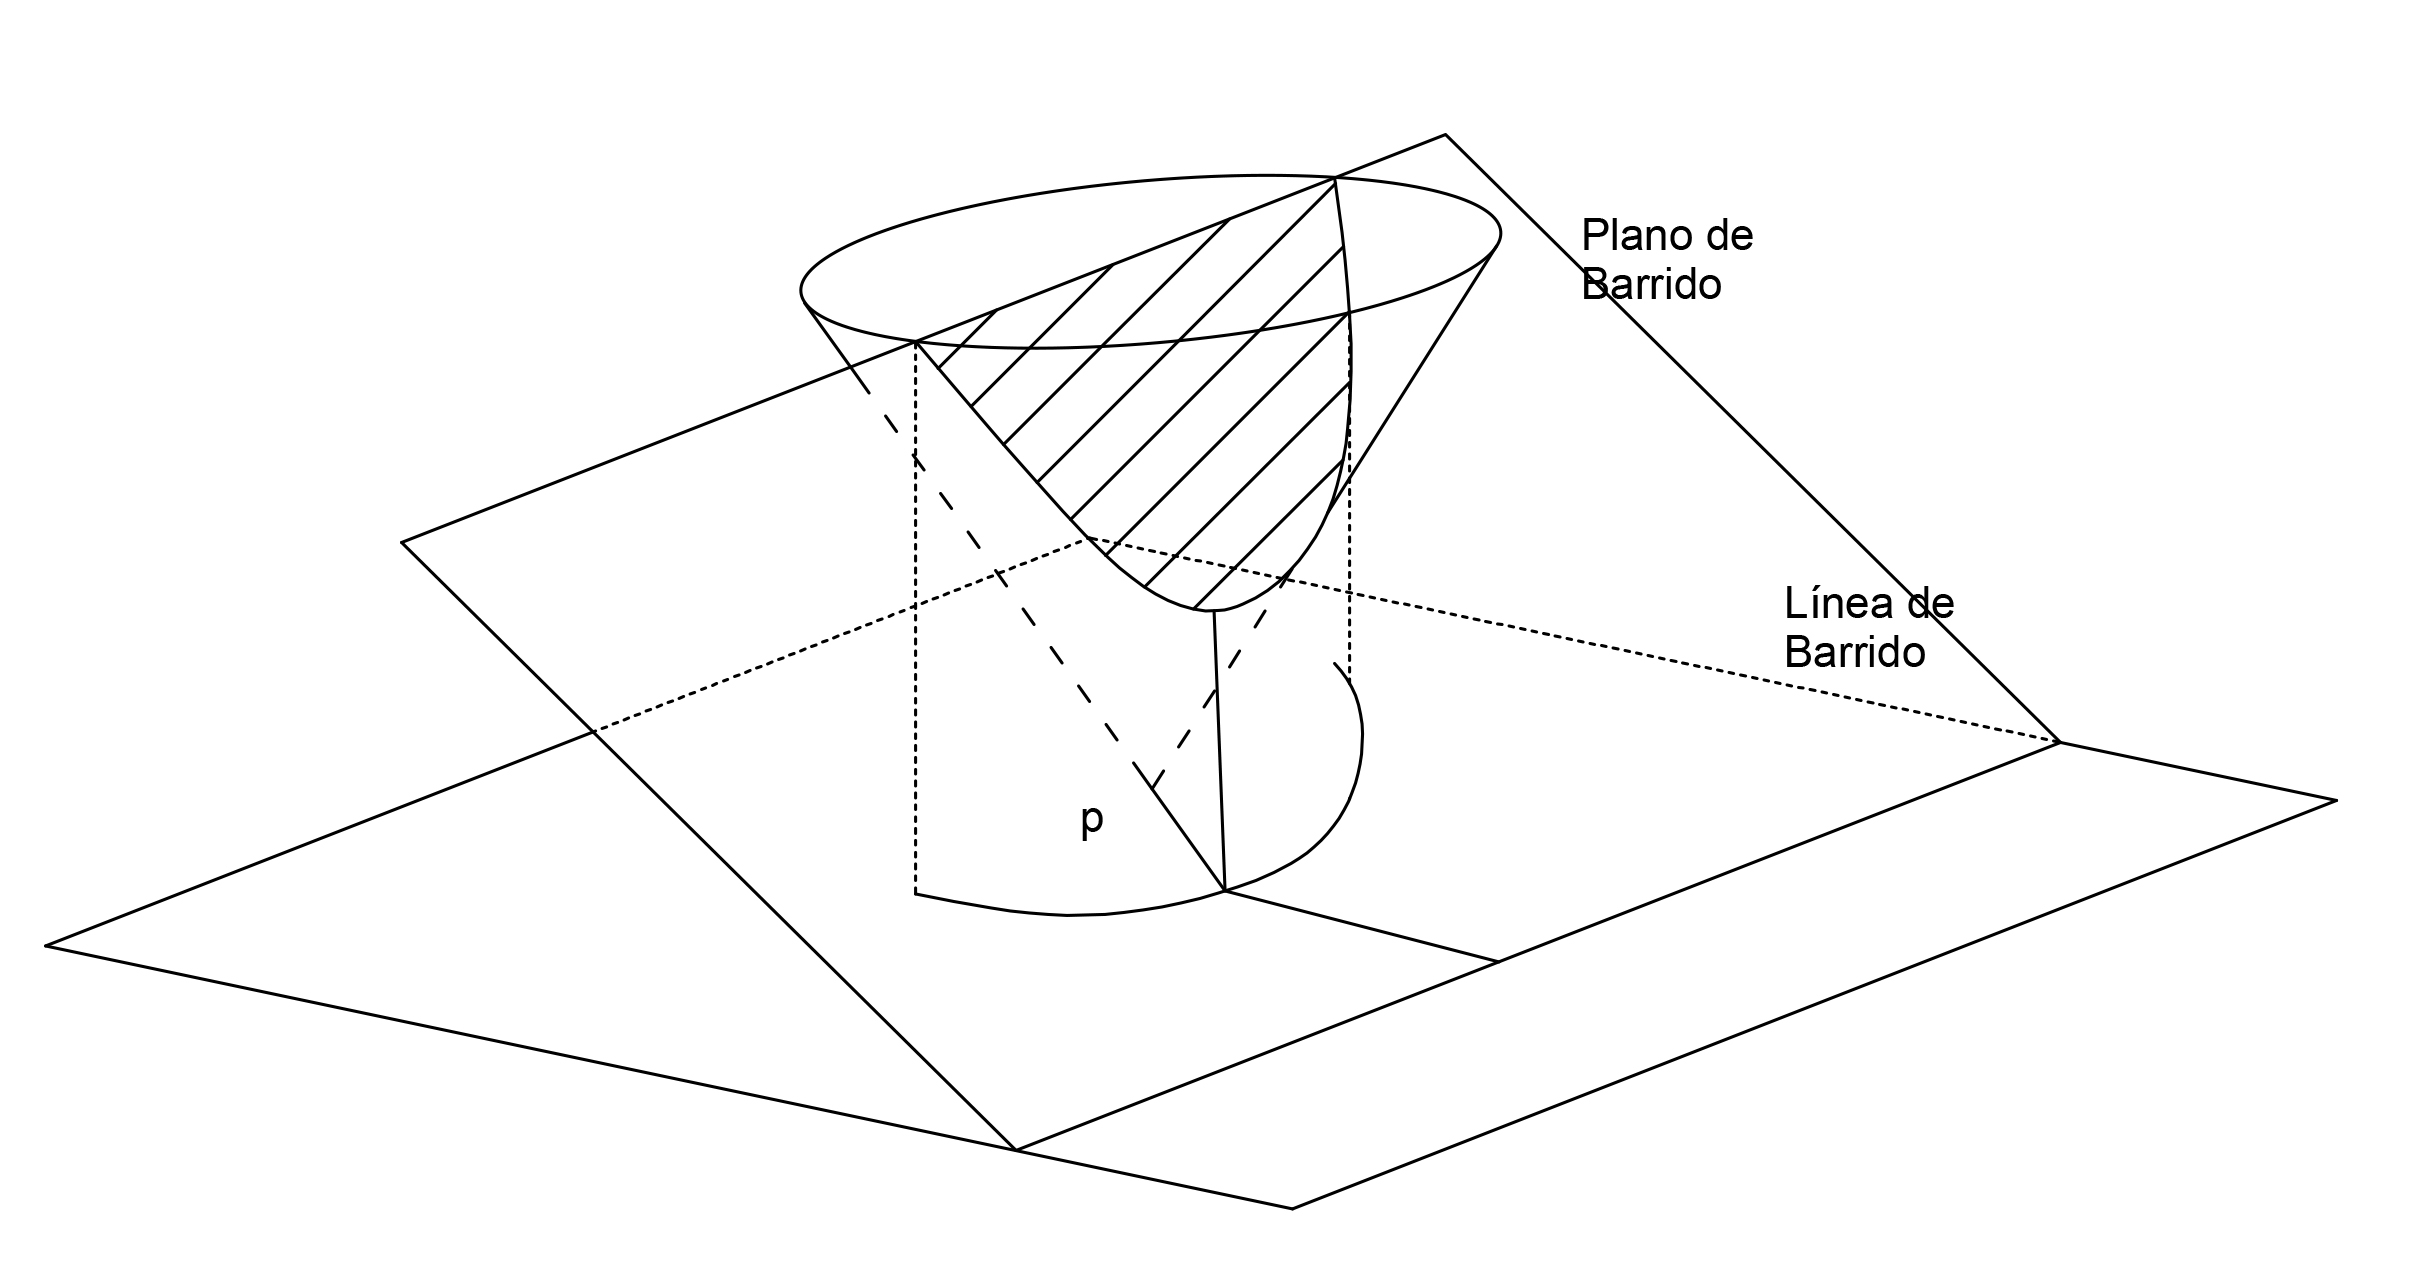
\includegraphics[scale=0.35]{imagenes/fortune4.jpg}
    } 
    \subfigure[Proyección en el eje $x-y$.]{
        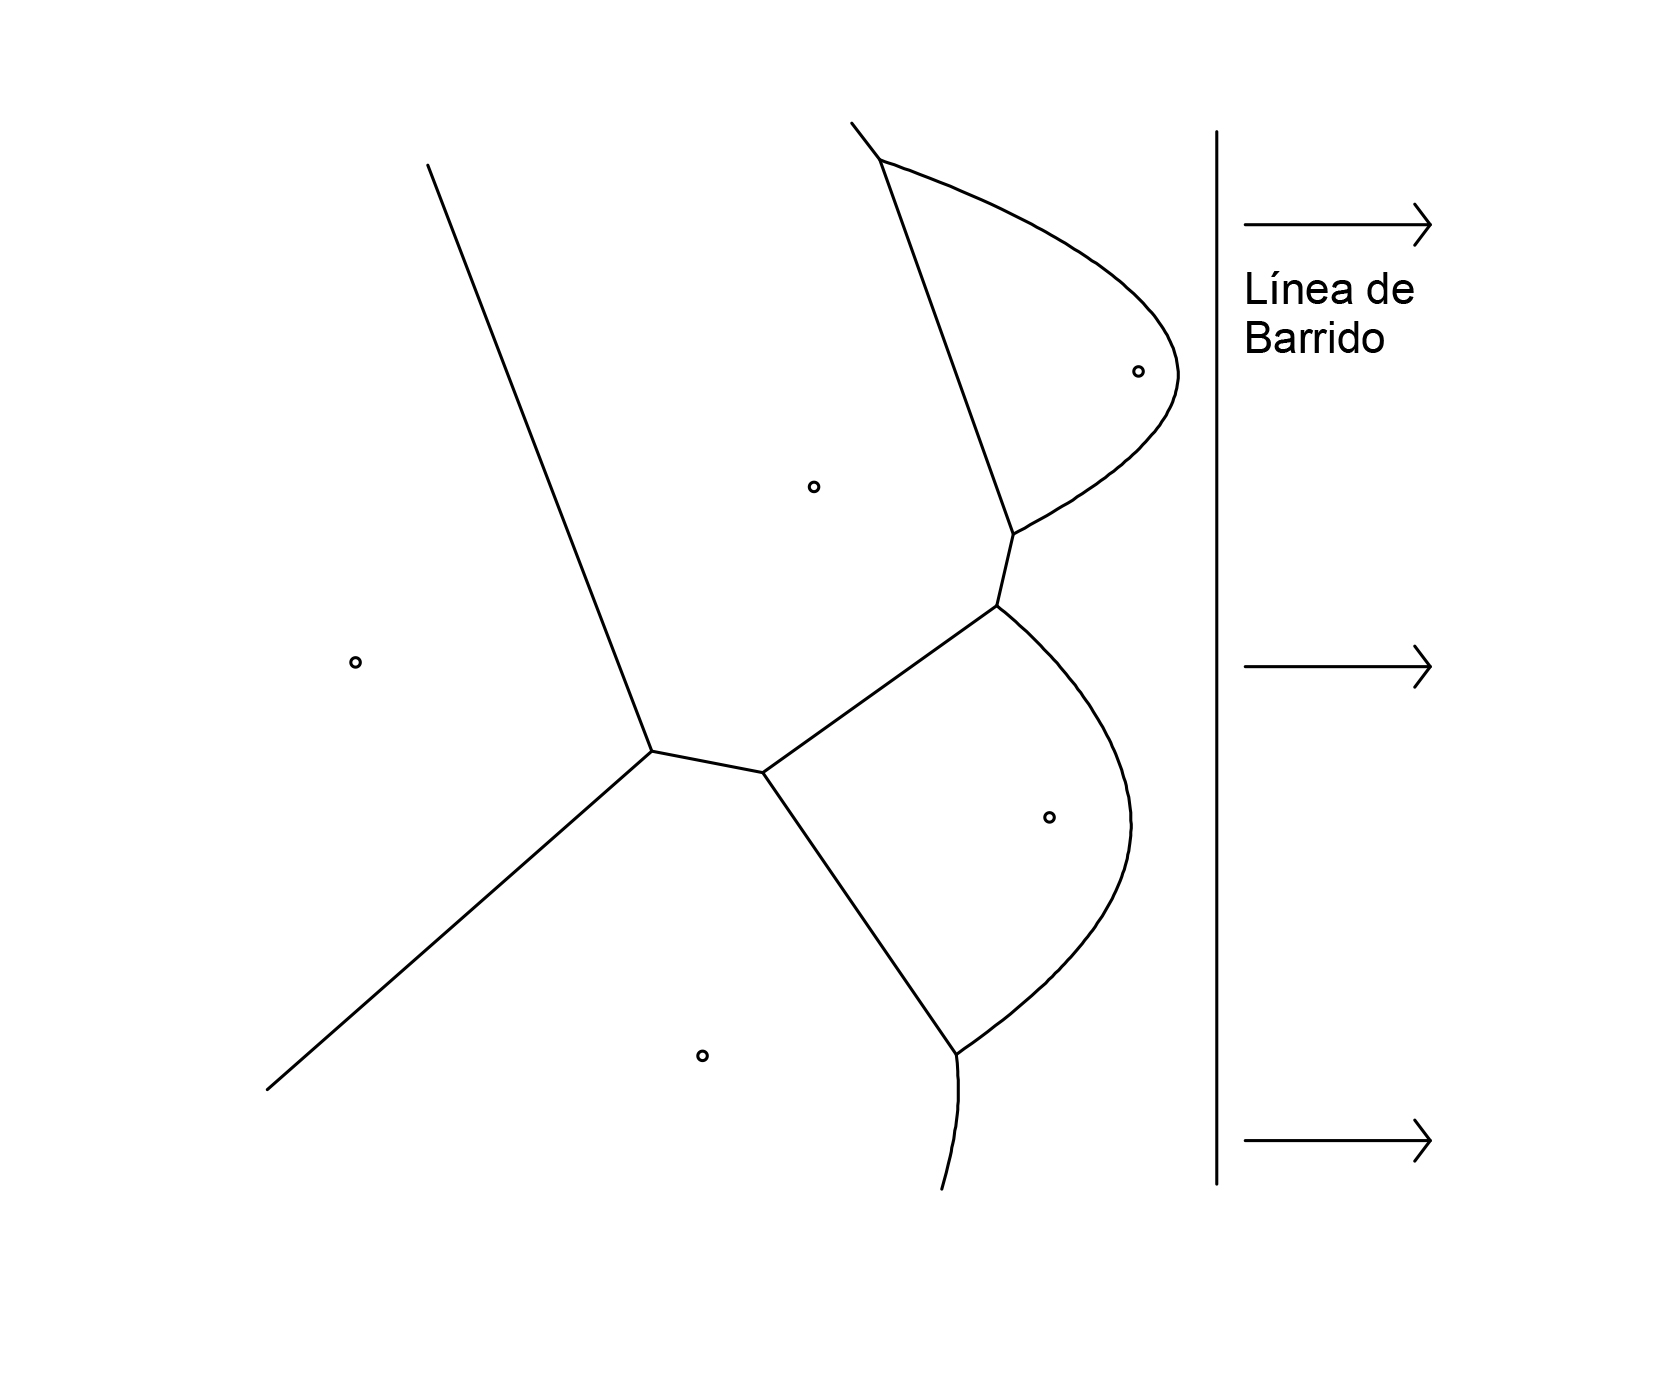
\includegraphics[scale=0.35]{imagenes/fortune1.jpg}
    }
    \begin{center}
        \subfigure[La frontera de la unión de todas las parábolas es lo que se denomina frente parabólico o línea de playa.]{
            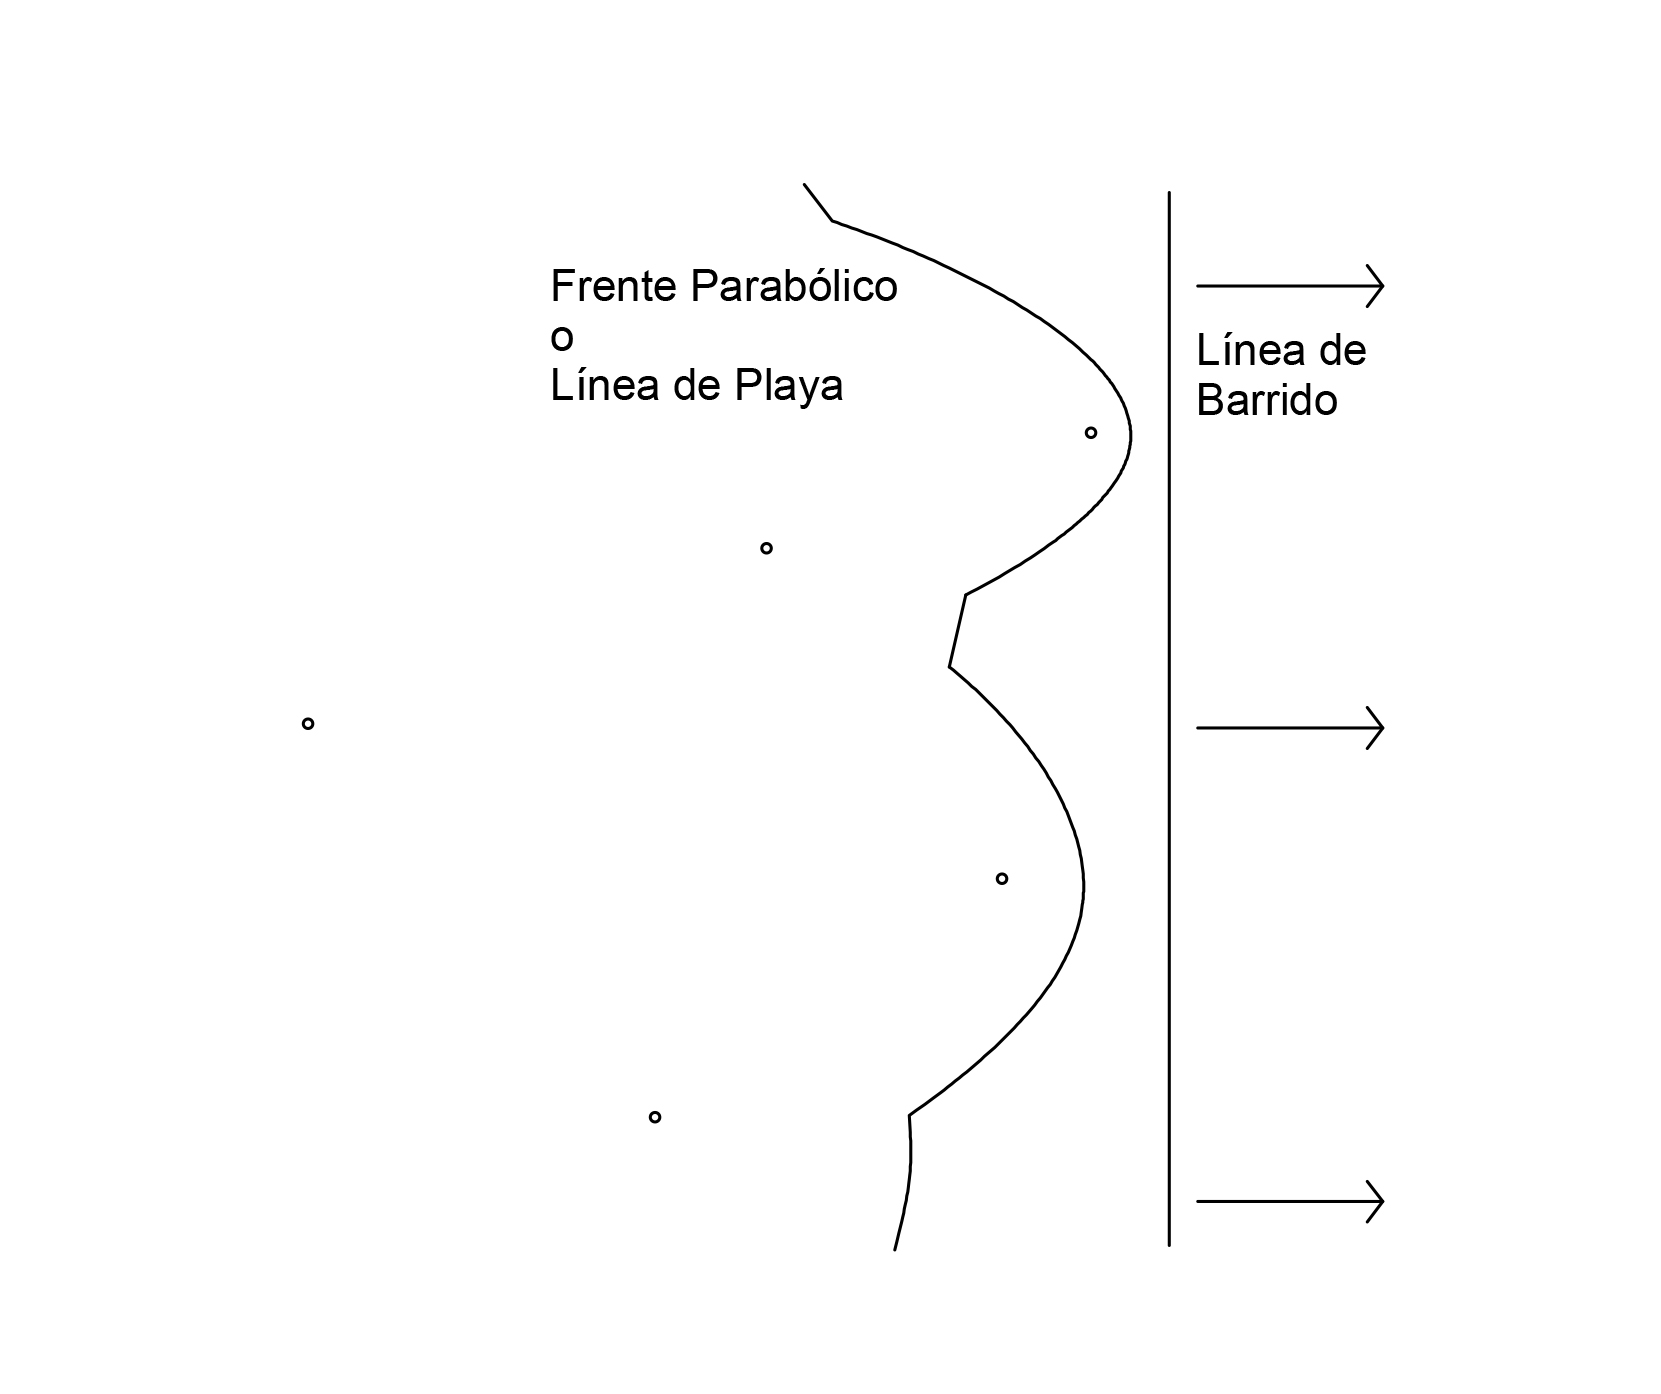
\includegraphics[scale=0.4]{imagenes/fortune2.jpg}
        }
    \end{center}
    \caption{Mecanismo de barrido del Algoritmo Fortune. } \label{fig:incre} 
\end{figure} 

Nos damos cuenta que a la izquierda, el plano de barrido está por encima de algunos conos y no bloquea sus vistas desde abajo. Sin embargo, hacia la derecha, como el plano de barrido es opaco, oculta todos los conos y no permite su visión desde abajo.
Si observamos por debajo del plano $x-y$, cada arco del frente parabólico cae en una región de Voronoi y cada punto de corte entre dos arcos consecutivos del frente parabólico cae en uno de los lados del Diagrama de Voronoi. Es decir, cada punto de un lado del Diagrama de Voronoi será un punto de corte entre dos arcos consecutivos del frente parabólico.
\vspace{0.3cm}

En la evolución del frente parabólico surgen dos tipos de eventos (\cite{fotosfortune}):
\begin{enumerate}
    \item Eventos de Sitio \\
        Cuando la línea de barrido pasa justo por encima de un punto, una parábola degenerada se une al frente parabólico y parte un arco de dicho frente en dos. La evolución posterior de la parábola durante el proceso de barrido dará lugar a una nueva arista del Diagrama de Voronoi.
        Por tanto diremos que hay un evento de punto cuando la línea de barrido pasa justo por encima de uno de los puntos de la nube. Este es el único modo de añadir un nuevo arco al frente parabólico y provoca la aparición de un nuevo lado del Diagrama de Voronoi.
        
        \begin{figure}  [H]
            \centering
            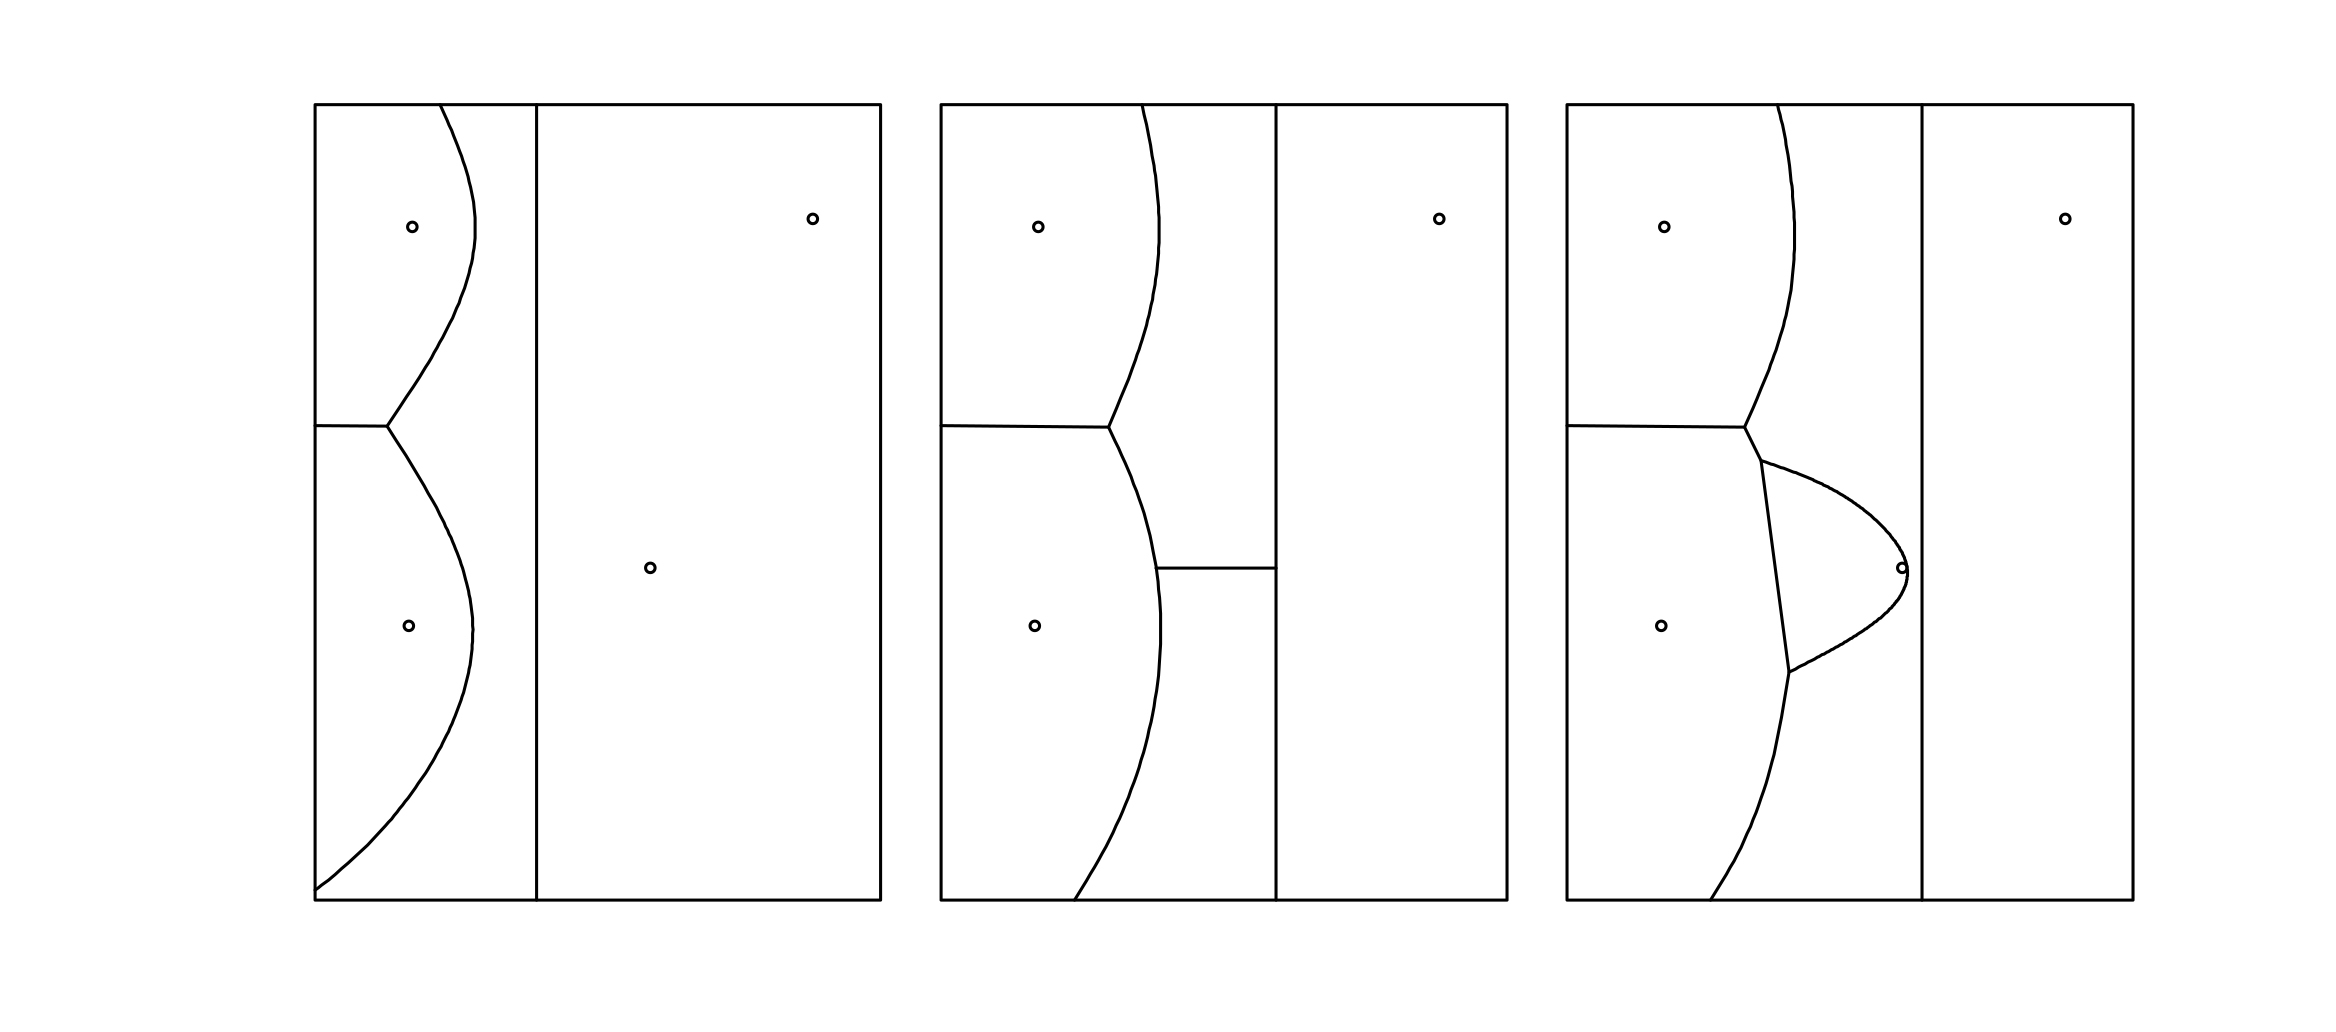
\includegraphics[scale=0.7]{imagenes/eventopuntos.jpg}
            \caption{Creación de una arista de Voronoi.}
        \end{figure}
        
    \item Eventos de Círculo \\
        Ocurre cuando un arco va decreciendo en el frente parabólico hasta convertirse en un punto y desaparecer de dicho frente.
        
        \begin{figure}  [H]
            \centering
            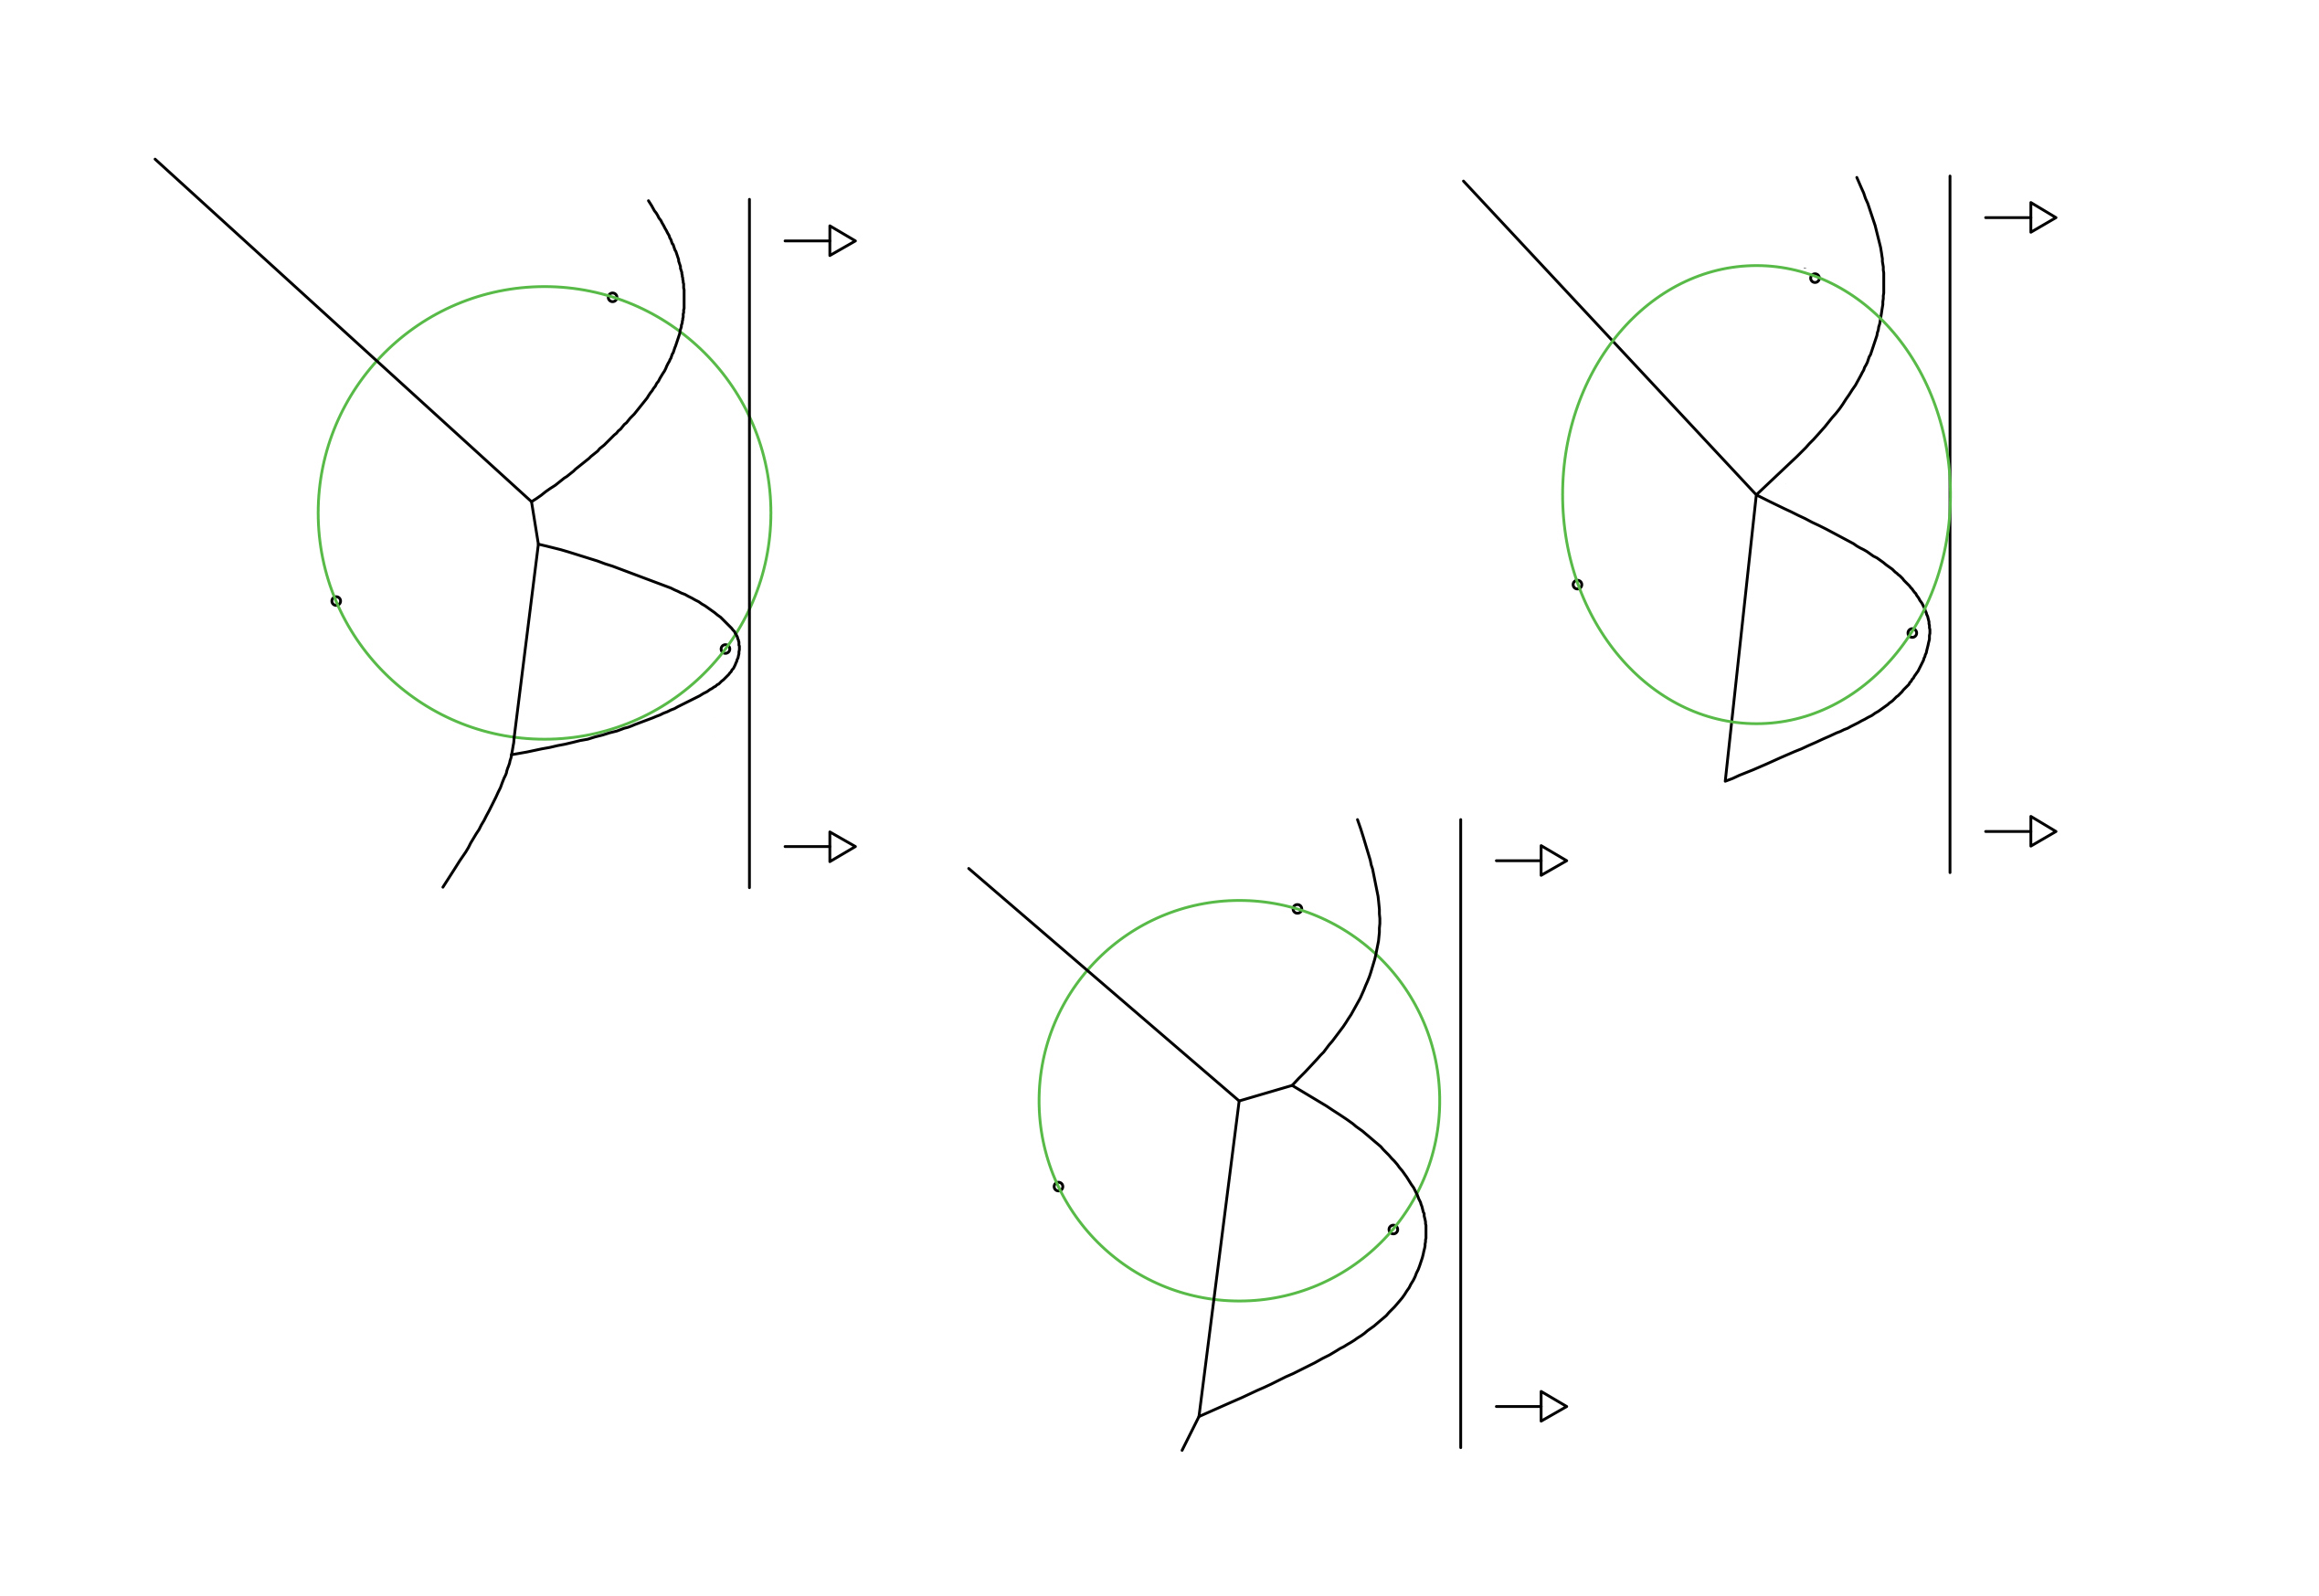
\includegraphics[scale=0.7]{imagenes/eventocirculos.jpg}
            \caption{Desaparición de un punto del frente parabólico.}
        \end{figure}
\end{enumerate}

El pseudocódigo de este algoritmo, que necesita tres tipos de estructuras de datos (estructura para guardar la parte del diagrama calculada hasta el momento; cola de prioridades que permita guardar los eventos de sitio y de círculo que debe procesar la línea de barrido; árbol de búsqueda binario que guarde la línea de playa) sería el siguiente (\cite{fotosfortune}):


    Entrada: $S:={s_{1},...,s_{n}}$ un conjunto de $n$ puntos en el plano.
    Salida: El Diagrama de Voronoi $V(S)$ dentro de un rectángulo de restricción.
    
    \begin{itemize}
        \item Inicializar la cola de eventos $Q$ con todos los puntos.
        \item Mientras $Q$ no esté vacío.
        \item Hacer considerar el evento con mayor coordenada $y$ de $Q$.
        \item Si el evento es un Evento de Sitio $s_{i}$,
            entonces TratarEventoSitio($s_{i}$).
        \item En caso contrario TratarEventoCirculo($s_{l}$), donde $s_{l}$ es el punto más bajo del círculo que causa el evento.
        \item Eliminar el evento de $Q$.
        \item Los nodos internos presentes todavía en $T$ (Árbol binario) pertenecen a las medio-aristas infinitas del Diagrama de Voronoi.
    \end{itemize}
    
    Calcular un rectángulo que contenga todos los vértices del Diagrama de Voronoi en su interior, uniéndole las semi-aristas infinitas.

\vspace{0.3cm}

Podemos observar, finalmente, que la técnica de barrido del plano reduce un problema estático bidimensional (por ejemplo, la construcción de un Diagrama de Voronoi en el plano) a un problema dinámico unidimensional (aquí, el mantenimiento de la representación de frente parabólico en la línea de barrido). Esto nos permite utilizar eficientes estructuras de datos unidimensionales como árboles binarios balanceados y colas de prioridad.


\section{Problemas de implementación}

Veamos cuáles son las cuestiones de implementación, incluidas las configuraciones degeneradas que podrían ocurrir en la entrada o durante la ejecución de dichos algoritmos, junto con las preguntas numéricas generales que surgen en el cálculo de objetos geométricos. 

\vspace{0.3cm}

Los problemas numéricos son las grandes (pero no las únicas) cuestiones críticas en este contexto, en la geometría computacional y en la computación geométrica y científica en general. 
Las decisiones basadas en las preguntas como las siguientes: ¿Son dos rectas exactamente paralelas, o se cruzan en un punto lejano remoto? ó ¿Podemos estar seguros de que este segmento de línea toca la circunferencia de ese círculo?, podrían influir críticamente en el posterior control del flujo de un algoritmo geométrico, y con él su exactitud o, peor aún, su corrección.

\vspace{0.3cm} 

El trabajo teórico de los algoritmos geométricos está a menudo basado en las siguientes suposiciones idealistas y, a veces, poco realistas: 

\begin{enumerate}
    \item Las entradas están en posición general.
    
        Se utiliza para descartar configuraciones de entrada degeneradas que se desvían del caso genérico y tienden a complicar las cosas. Por ejemplo, si asumimos que no hay tres puntos en el conjunto $\mathcal{S}$ que coinciden en una línea, y no cuatro puntos en un círculo, entonces la teselación de Delaunay es siempre una triangulación de $\mathcal{S}$. Que las configuraciones descartadas están contenidas en un subconjunto de menor dimensión del espacio de configuración $R^{2n}$ de las coordenadas del punto parece ser una justificación suficiente para ignorarlas. No obstante, en la aplicación de integración a escala muy grande (VLSI), el conjunto de entrada puede consistir en puntos de rejilla que no estén en posición general. En consecuencia, tenemos que implementar algoritmos de tal manera que puedan hacer frente a todas las entradas posibles. Hay diferentes maneras de proceder.
        \vspace{0.3cm}
        
        Comenzando con un algoritmo que trabaja para la entrada en la posición general, uno podría también extenderse en un algoritmo que pueda manejar la entrada degenerada. A veces esto puede hacerse de una manera orgánica, sin implementar análisis de casos complicados. Por ejemplo, el algoritmo divide y vencerás se puede extender para manejar los vértices de Voronoi de grado mayor que 3. Calcula el Diagrama de Voronoi para $n$ puntos arbitrarios en el plano $\mathcal{S}$, por lo tanto por dualización.
        \vspace{0.3cm}
        
        Otra aproximación elegante se basa en la idea de que mover los puntos en S por una cantidad infinitesimal eliminará las degeneraciones como las mencionadas anteriormente. Por lo tanto, primero se aplica una perturbación a la entrada de tal manera que se consigue la posición general. Entonces el algoritmo se ejecuta en la entrada perturbada. Una dificultad consiste en recuperar la salida verdadera en la entrada S, a partir de la salida que A ha calculado sobre la entrada perturbada.


    \item La aritmética del número real es exacta y puede realizarse en tiempo constante.
    
        La mayoría de los lenguajes de programación ofrecen valores estandarizados de punto fijo o flotante, con un número predefinido de dígitos, números enteros de tamaño fijo y enteros de longitud (potencialmente) ilimitada. Mientras que la aritmética de coma flotante está soportada por hardware y, por lo tanto, es bastante rápida pero propensa a errores de redondeo. La computación con enteros largos, por otro lado, es exacta pero lenta. Un enfoque de filtro de punto flotante intenta evitar cálculos enteros largos, utilizando aritmética de punto rápido en combinación con límites de error.
        \vspace{0.3cm}
        
        Si los objetos de entrada se especifican mediante coma flotante o coordenadas racionales, pueden representarse exactamente por los tipos de números anteriores. Sin embargo, tan pronto como un algoritmo genera nuevos objetos geométricos a partir de los dados, sus coordenadas no necesitan ser números racionales. Por ejemplo, el algoritmo de barrido del plano genera vértices de Voronoi como puntos de intersección de parábolas. Sus coordenadas envuelven raíces cuadradas. Bisecciones de objetos curvos más generales pueden ser de mayor grado algebraico.
        
        
        En general, es necesario encontrar los ceros reales de las ecuaciones polinomiales con coeficientes racionales $a_{i}$.
        
        \begin{center} $f(x) =  \displaystyle\sum_{i=0}^n a_{i}x^i$ \end{center}
        
        Si el grado de $n$ es mayor que 4, los ceros de $f$ pueden, en general, no ser expresados por radicales anidados en los números $a_{i}$. 
        
        En su lugar, los ceros reales de $f$ deben aislarse por intervalos racionales, y luego ser numéricamente aproximados. El problema se vuelve aún más difícil si los coeficientes $a_{i}$ son números algebraicos, sólo disponibles por aproximación. Ambas cuestiones, degeneración y precisión, se entrelazan. A saber, muchos algoritmos geométricos proceden evaluando predicados geométricos. 
        

\end{enumerate}
Este tema sobre los problemas de implementación que pueden originar los diferentes algoritmos disponibles para la computación de los Diagramas de Voronoi es bastante amplio y se puede ahondar mucho más en él pero no es el tema central de este trabajo. No obstante, puede ser interesante la consulta de ciertos libros que se adentran en todas estas cuestiones que hemos mencionado, como pueden ser: Seidel \cite{seidel} para la primera suposición;  Mehlhorn y Näher \cite{mys} y Yap \cite{yap} para la segunda.

\vspace{0.3cm}


\chapter{Desarrollo de la Librería} \label{capi6}

En este capítulo nos centraremos en hacer toda la representación gráfica ya que es la manera más vistosa para entender el funcionamiento de estos diagramas y todo lo referente a nuestro trabajo. La condición de Delaunay es posible ampliarla para espacios tridimensionales usando la esfera circunscrita en vez de la circunferencia circunscrita y, aunque también es posible ampliarla para espacios con más dimensiones, no se usa en la práctica. 
Por otro lado, la técnica del algoritmo incremental es la que utilizaremos para realizar la Triangulación de Delaunay (Edelsbrunner y Shah \cite{edelshah}).
Un buen software en el que podemos ver ejemplos de cálculo de la envolvente convexa, la Triangulación de Delaunay, el Diagrama de Voronoi, la intersección de medio espacio alrededor de un punto, la Triangulación de Delaunay del sitio más lejano y el Diagrama de Voronoi del sitio más lejano es Qhull, \cite{qhull}, donde el código fuente se ejecuta en 2-d, 3-d, 4-d y dimensiones superiores.

\begin{comment} --------------- 6.1 --------------- \end{comment}

\section{Análisis de requisitos}

Para comenzar con esta parte informática, elaboraremos un documento de descripción del sistema que recogerá detalladamente el comportamiento del mismo, los datos que recibe, trata, almacena y devuelve, y cualquier consideración sobre su funcionamiento. Además, haremos un análisis de requisitos donde habrá que distinguir los requisitos correspondientes a cada área funcional: los \textbf{requisitos de datos} serán los datos que hay que comunicar al sistema, qué almacena y qué devuelve; los \textbf{requisitos funcionales} que van a ser las funciones que tiene que realizar el sistema. Registraremos un requisito por cada función puntual del sistema; las \textbf{restricciones semánticas} recogen el funcionamiento especial del sistema.
\vspace{0.3cm}

Deseamos implementar una librería para la gestión de Diagramas de Voronoi mediante el lenguaje de programación Java (\cite{java2}) y haciendo uso, además, como complemento, de otro lenguaje de programación como es Python (\cite{python}). Con ello pretendemos facilitar información a todo aquel interesado en el estudio de estos diagramas. Nuestro objetivo será realizar una aplicación multimedia que permita trabajar con la entrada de coordenadas de puntos (tanto con eventos de ratón, como indicando las coordenadas manualmente) para dibujar Diagramas de Voronoi, su correspondiente triangulación y las circunferencias circunscritas de cada triángulo formado. Debemos ilustrar gráficamente, si la dimensión nos lo permite, estas estructuras en tiempo real o, por el contrario, si la dimensión es elevada, la indicaremos junto con las coordenadas de los puntos mediante un fichero de texto y mostraremos el resultado en otro fichero generado por nuestra aplicación, indicando los vértices y las regiones de Voronoi formadas a partir de esos puntos. 

\subsection{Requisitos específicos}

Será necesario disponer de una versión actualizada (en mi caso, lo he ejecutado siempre con la versión 1.8) de Java \cite{java}. Además, será necesario tener instalado Python \cite{python} así como su librería SciPy \cite{pythonclass} para poder ejecutar la aplicación de terminal para dimensiones elevadas.

\subsection{Requisitos funcionales}

Contamos con una lista de las funciones que tiene que realizar nuestro sistema. 

\begin{itemize}
    \item[\ding{224}] Crear Ventana: El sistema debe generar una ventana vacía a la que añadirle un lienzo.
    \item[\ding{224}] Crear un lienzo vacío: El sistema generará un lienzo con el fondo vacío cuyo tamaño será el del triángulo inicial utilizado para el algoritmo incremental.
    \item[\ding{224}] Nuevo lienzo vacío: Poder generar una nueva ventana con un lienzo en blanco.
    \item[\ding{224}] Cuadro de diálogo para abrir un fichero: Mediante un cuadro de diálogo permitir abrir un fichero de texto que tenga la entrada requerida.
    \item[\ding{224}] Dibujar Voronoi en el Lienzo: El sistema dibujará los puntos indicados en el fichero de entrada y representará el Diagrama de Voronoi correspondiente.
    \item[\ding{224}] Cuadro de diálogo para guardar un fichero: El sistema abrirá un cuadro de diálogo en el que el usuario indica el nombre y la ruta donde almacenar el fichero y lo guardará con el mismo formato que el fichero de entrada, donde se indicará lo que tengamos actualmente dibujado.
    \item[\ding{224}] Cuadro de diálogo para exportar un fichero: El sistema abrirá un cuadro de diálogo en el que el usuario indica el nombre y la ruta donde almacenar el fichero y lo guardará con el formato necesario para poder reproducir lo que haya actualmente en el lienzo.
    \item[\ding{224}] Cambiar herramienta: El sistema cambiará la herramienta de Dibujo del lienzo por la nueva, que será: dibujar triangulación de Delaunay, dibujar circunferencias circunscritas o pintar el camino más corto entre dos puntos elegidos de manera aleatoria.
    \item[\ding{224}] Establecer escala: Aplicar escalado al diseño, aumentando o disminuyendo la escala y permitiendo seguir dibujando en él.
    \item[\ding{224}] Introducir coordenadas: Existirán dos cuadros para indicar las coordenadas de un punto y que éste se dibuje en el lugar indicado.
\end{itemize}

\subsection{Requisitos de datos}

A continuación detallamos una lista numerada de los datos que hay que comunicar al sistema, qué almacena y qué devuelve. 

\begin{itemize}
    \item[\ding{224}] Entrada: Dimensión.
    \item[\ding{224}] Entrada: Número de puntos sobre los que queremos que se construya el Diagrama de Voronoi.
    \item[\ding{224}] Entrada: Coordenadas de dichos puntos.
    \item[\ding{224}] Manejo: Mostrar los puntos indicados, dibujando su Diagrama de Voronoi, dando la oportunidad a añadir otros.
    \item[\ding{224}] Manejo: Abrir un archivo de texto en el que se indique como entrada la dimensión, el número de vértices y las coordenadas de cada punto.
    \item[\ding{224}] Manejo: Guardar la entrada de puntos realizada en un fichero de texto con el mismo formato que el de entrada (dimensión, número de puntos y coordenadas de los puntos). 
    \item[\ding{224}] Manejo: Exportar en un documento la información necesaria para que cualquier persona pueda dibujar el Diagrama de Voronoi representado. Esto es, las coordenadas de los vértices de Voronoi, identificados con un índice, para los puntos introducidos y mostrar una matriz que indicará si están conectados dichos vértices (0 si no están conectados y 1 si lo están).
    \item[\ding{224}] Manejo: Mostrar en todo momento las coordenadas en las que nos encontremos. 
    \item[\ding{224}] Manejo: Permitir acercar o alejar lo representado para verlo con claridad.
    \item[\ding{224}] Manejo: Opción de empezar de nuevo sin tener que reiniciar la aplicación diseñada.
    \item[\ding{224}] Salida: Representación gráfica del Diagrama de Voronoi, la Triangulación de Delaunay y sus circunferencias circunscritas.
    \item[\ding{224}] Salida: Establecer el camino más corto entre dos puntos elegidos de manera aleatoria, pasando por las aristas del Diagrama de Voronoi, a las que se accederá trazando líneas perpendiculares hacia ellas y alejándose de los puntos únicos de cada región (los que forman la Triangulación de Delaunay).
    \item[\ding{224}] Salida: Sendos ficheros de texto para utilizar en la aplicación y para que cualquier otra persona pueda elaborar el Diagrama de Voronoi representado.    
\end{itemize}


\subsection{Restricciones semánticas}
\begin{itemize}
    \item[\ding{224}] Para el diseño de nuestra solución además se nos exige elaborar la aplicación utilizando el lenguaje de programación Java, permitiéndonos utilizar todas las librerías disponibles.
    \item[\ding{224}] Utilizar el algoritmo incremental para generar la Triangulación de Delaunay.
    \item[\ding{224}] Además de realizar la interacción de ficheros con los botones necesarios, establecer un comando directo a través del teclado.  
    \item[\ding{224}] El Diagrama de Voronoi de los puntos se dibujará siempre por defecto y en todo momento, representando todas las demás opciones (Triangulación de Delaunay, circunferencias y camino más corto) con dicho diagrama representado.
    \item[\ding{224}] Las regiones de Voronoi se diferenciarán representándolas de distintos colores establecidos de manera aleatoria.
\end{itemize}

    

\section{Diseño de la solución}

En primer lugar, se ha desarrollado una librería en Java cuya utilización, por un lado, nos va a permitir, al pasarle un fichero de texto con extensión .txt con la entrada correspondiente, la salida deseada también en un archivo "salida.txt" lo que haremos para la dimensión dos en el lenguaje de programación Java y para dimensiones superiores utilizando un fichero elaborado en el lenguaje de programación Python (incluido en nuestra aplicación de Java). Es decir, partiremos de un problema en el que los datos de entrada serán: la dimensión, el número de puntos y las coordenadas de cada punto. Las salidas que obtendremos serán las coordenadas de los vértices de Voronoi y el número de polígonos creados (regiones de Voronoi). Ésta será la primera aplicación desarrollada. Por otro lado, dicha librería ha sido incluida en otro proyecto de Java donde se desarrolla, con la utilización de un JFrame y un JPanel, la visualización del Diagrama de Voronoi y una aplicación que hemos considerado que puede hacer que, de manera visual, se entienda perfectamente el cálculo de los diagramas y el gran uso que pueden tener.
\vspace{0.3cm} 

Decidimos que ésta era la manera idónea de programar todo. Es decir, teniendo, por un lado, la librería necesaria para utilizar Voronoi, no sólo para las aplicaciones que hemos implementado en 2D, sino para usos futuros o para cualquier otro usuario interesado en utilizarla. Por otro lado, la aplicación para interactuar con la terminal. Y, por último, incluyendo la librería en un JFrame y con el uso de un JPanel incluidos en java, poder elaborar la interfaz gráfica.
\vspace{0.3cm} 

En la librería realizada, se pueden distinguir una serie de clases, que serán la base de todo lo que hagamos. Además, esta librería podría ser utilizada para posibles aplicaciones futuras. Las clases son las siguientes:

\begin{itemize}
    \item \textbf{Punto}: En esta clase, consideramos los puntos en el espacio Euclídeo y los implementamos como \textit{double} (números reales). Incluiremos operaciones geométricas básicas que se pueden realizar con los puntos como son: obtener sus coordenadas y su dimensión, crear un nuevo punto a partir de otro añadiéndole coordenadas, producto escalar, norma, suma, resta, cálculo del ángulo y la bisectriz. Por otro lado representaremos las matrices y las envolventes convexas como un \textit{array} (estructura de datos que nos permite almacenar una gran cantidad de datos de un mismo tipo) de puntos. Para las matrices calculamos tanto el determinante como el producto matricial. Para los símplices o envolventes convexas vemos qué relación mantienen con los puntos, es decir, si éstos están dentro, fuera o incluidos. Del mismo modo veremos qué relación tienen con las circunferencias circunscritas y calcularemos el circuncentro.
    \item \textbf{Conjunto}: Hereda de una clase abstracta, \textit{AbstracSet}, que proporciona una implementación esquelética de la interfaz \textit{Set} para minimizar el esfuerzo requerido para desarrollarla. Además, haremos uso de la clase \textit{Collections}, también incluida en el paquete de Java, que consiste enteramente en métodos estáticos que se utilizan para operar en colecciones. Operaciones comunes como ordenar una lista o encontrar un elemento de una lista se pueden hacer fácilmente usando dicha clase. Con su uso, la clase Conjunto nos permite: crear un conjunto vacío de tamaño 3; crear un conjunto con la capacidad que le digamos; crear un conjunto que contenga los elementos de la colección, eliminando los duplicados; devolver el elemento del índice que le especifiquemos; comprobar si algún elemento de la colección también pertenece a este conjunto.
    \item \textbf{Triángulo}: Hereda de la clase Conjunto. Un triángulo va a ser un conjunto no modificable de exactamente 3 puntos. Nos va a permitir calcular cuáles son los triángulos vecinos; obtener la cara opuesta a un vértice que le indiquemos y obtener el circuncentro calculado en la clase Punto. 
    \item \textbf{Grafo}: En esta clase los nodos van a tener un tipo genérico G. Añadimos y eliminamos tanto nodos como aristas en el grafo no dirigido. Además, podemos obtener el conjunto de nodos de dicho grafo. Hemos empleado, para su implementación, la clase \textit{Collections} explicada anteriormente para definir un conjunto de nodos; y las clases \textit{HashMap}, que es una clase rápida y fácil de usar que representa una tabla hash (estructura de datos que asocia las claves con valores) y \textit{Maps} cuya interfaz asigna las claves a los valores. Las claves son únicas y por lo tanto, no se permiten claves duplicadas. Estas últimas serán las que nos permitan crear la variable \textit{vecinos} que nos ayudará a saber qué nodos son los más cercanos a uno dado.
    \item \textbf{Triangulación2D}: Realizamos la Triangulación de Delaunay en dos dimensiones mediante el algoritmo incremental \ref{incremental}. Ésta no es la manera más rápida de construirlo, pero es una manera razonable de construir una Triangulación de Delaunay incrementalmente y permite una buena visualización interactiva. Consideramos la triangulación como un conjunto de triángulos no modificable como conjunto. La única manera de cambiarla es añadiéndole sitios mediante uno de los métodos implementados. También podremos obtener el triángulo opuesto del vértice especificado; recorrer los triángulos alrededor de uno dado y podremos comprobar a qué triángulo pertenece un punto. 
    \item \textbf{Dijkstra}: Clase específica para implementar el \textbf{Algoritmo de Dijkstra} que calcula el camino optimal desde un punto hasta otro en un grafo, teniendo en cuenta los pesos de cada arista. En nuestro caso, los pesos serán la distancia euclídea entre ellos. La idea es buscar el punto más cercano posible a nuestro punto de origen, repitiendo el proceso hasta llegar a nuestro punto de destino, moviéndonos por los vértices y las aristas de Voronoi. Utilizaremos para implementarlo una cola de prioridad incluida en la clase \textit{PriorityQueue} de Java.
\end{itemize}
\vspace{0.3cm} 

En otro proyecto de Java hemos realizado, como ya hemos comentado, el diseño de la visualización del Diagrama de Voronoi, incluyendo la librería anteriormente explicada. Además, hemos empleado el algoritmo de Dijkstra que nos calcula el camino más corto posible entre dos puntos elegidos al azar. Esta aplicación puede ser útil, por ejemplo, en Robótica. Si tenemos una escena con obstáculos (atractores) en las que un robot deba moverse, una forma de evitar las colisiones o el acercamiento sería diseñar la trayectoria del robot sobre las líneas del Diagrama de Voronoi, con lo que se movería siempre a medio camino entre dos de los atractores, intentando acercarse lo menos posible a ellos. Esto es precisamente una de las aplicaciones que podremos visualizar de manera gráfica. En este proyecto hemos incluido lo siguiente:

\begin{itemize}
    \item \textbf{Lienzo}: Se trata de un JPanel en el que están implementados todos los métodos para poder dibujar tanto el Diagrama de Voronoi, como su respectiva Triangulación de Delaunay, además de las circunferencias circunscritas. Para ello, tendremos unos métodos básicos de dibujado con los que podremos dibujar puntos, aristas y los respectivos polígonos formados, añadiéndoles un color aleatorio que nos va a permitir distinguir con claridad las regiones de Voronoi. Por otro lado disponemos de otros métodos específicos de dibujado: para dibujar la Triangulación de Delaunay, recorremos todos los triángulos y vamos uniendo los diferentes vértices; para dibujar las circunferencias circunscritas recorremos los diferentes triángulos de la triangulación y calculamos sus circuncentros; en el dibujo de Voronoi debemos tener en cuenta que los circuncentros de las circunferencias serán nuestros vértices de Voronoi y calculamos la distancia euclídea entre vértices para saber cuáles de ellos están conectados. Además, tendremos en cuenta que en cada región de Voronoi sólo podrá haber un punto (vértice de los triángulos de la triangulación).
    Además, tenemos unos métodos específicos implementados para obtener el camino más corto posible entre dos puntos elegidos al azar utilizando el algoritmo de Dijkstra como son: la obtención del punto más cercano a otro punto; cálculo del punto más cercano a un segmento; añadir una arista que conecte los puntos de corte (que se encuentran en una misma arista de Voronoi) entre los dos puntos elegidos, en caso de que éstos se encuentren en regiones colindantes; añadir todas las perpendiculares al polígono en el que se encuentren dichos puntos, para después elegir la más adecuada para establecer el camino más corto.
    Por último, implementamos los métodos que nos van a permitir trabajar con ficheros (guardar, abrir, exportar) y un método que, según en el caso en el que nos encontremos, hará la función que le corresponda. Además aquí incluimos la gestión de eventos de ratón vinculados al proceso de dibujado.
    \item \textbf{VentanaPrincipal}: Se trata de un JFrame en el que incluimos el JPanel Lienzo. Por tanto, aquí simplemente establecemos qué deben hacer los botones añadidos a nuestra interfaz.
\end{itemize}

A continuación detallamos las opciones que existen en nuestra interfaz y en la sección siguiente \ref{manual} veremos cómo se utilizan:
\begin{itemize}
        \item \textbf{Modos}:
            \begin{itemize}
                 \item Voronoi: Ésta será la opción por defecto. Cada vez que hagamos click con el ratón, se pintarán unos puntos (tantos como queramos) y su respectivo Diagrama de Voronoi. Estos puntos serán los vértices de los triángulos que construyen la Triangulación de Delaunay y sólo habrá uno de ellos en cada región de Voronoi.
                 \item Dijkstra: Cuando este botón está seleccionado, automáticamente, el próximo click hecho con el ratón ya no será para construir el Diagrama de Voronoi, sino que se podrán elegir dos puntos aleatorios y se calculará el camino optimal más corto entre ellos, moviéndose por las aristas y vértices de Voronoi. Si volvemos a hacer click con el ratón se eliminará el camino y podremos volver a seleccionar dos puntos para volver a calcular este algoritmo.
            \end{itemize}
        \item \textbf{Más información}:
            \begin{itemize}
                \item Delaunay: Si este cuadro está seleccionado, podremos ver la Triangulación de Delaunay del respectivo Diagrama de Voronoi.
                \item Circunferencias: Al igual que el botón de Delaunay, si este botón está seleccionado, se mostrarán las circunferencias circunscritas correspondientes a la triangulación y al diagrama.
            \end{itemize}
        \item \textbf{Interacción con ficheros}:
            \begin{itemize}
                \item Abrir (Alt+A): Permite seleccionar un fichero de texto, en el que la entrada será la dimensión, el número de vértices y sus correspondientes coordenadas. La interfaz dibujará esos puntos por defecto, permitiendo incluir algunos más si así lo deseamos. 
                \item Guardar (Alt+G): Permite guardar en un fichero de texto los mismos datos de entrada (dimensión, número de vértices y coordenadas de dichos vértices) para, en caso de usar posteriormente el botón de abrir para seleccionar el archivo guardado, pudiéramos volver a mostrarlo.
                \item Exportar (Alt+E): Permite guardar un archivo con la misma extensión que los anteriores (.txt) que incluirá la información necesaria para dibujar el Diagrama de Voronoi que acabamos de mostrar en pantalla. Dicha información será una lista de los vértices de Voronoi generados con un índice para identificarlos y una matriz de aristas que indicará si dichos vértices están relacionados o no (mostrando 1 ó 0 respectivamente).
             \end{itemize}
        \item \textbf{Otras opciones}:
            \begin{itemize}
                \item Limpiar (Alt+L): Borra todo lo realizado, dejando el fondo blanco, dando la oportunidad de volver a dibujar de nuevo.
                \item Ver: Nos permite ocultar la barra de herramientas si así lo deseamos.
                \item Zoom: Habrá en nuestra interfaz una barra de desplazamiento que podemos deslizar para acercar o alejar el Diagrama de Voronoi que hayamos dibujado. 
                \item Añadir: Podremos añadir puntos, además de haciendo click con el ratón, indicando las coordenadas X e Y y pulsando el botón, de manera automática, se nos dibujará el punto que hayamos introducido.
           \end{itemize}        
        \item Además, en la parte de abajo de nuestra interfaz se mostrarán las coordenadas de los puntos por los que vayamos pasando con el ratón.
\end{itemize}

Estas dos aplicaciones, tanto la de entrada y salida de ficheros como la que utiliza una interfaz gráfica, han sido incluidas en un archivo JAR, que permite ejecutar aplicaciones escritas en el lenguaje Java y Python. Con Java instalado en nuestro ordenador bastará con abrir la terminal y escribir por línea de comandos las siguientes órdenes para ejecutar los .jar correspondientes:
 \begin{itemize}
        \item Aplicación Voronoi + Dijkstra: java -jar VoronoiDijkstraApp.pack.jar
        \item Aplicación entrada y salida: java -jar VoronoiTerminal.pack.jar entrada.txt
\end{itemize}

A continuación mostraremos ejemplos de uso de estas aplicaciones donde podremos ver su funcionamiento de manera gráfica.

\section{Manual de usuario} \label{manual}

Aunque el diseño gráfico es bastante intuitivo, vamos a ver con ejemplos cómo utilizar las dos aplicaciones diseñadas.
\vspace{0.3cm} 

\begin{itemize} 
    
    \item Empezaremos por la que interactúa directamente con la terminal, sin hacer uso de ninguna interfaz gráfica.
\end{itemize}
    
    \begin{enumerate}
        \item Tras abrir la terminal de Windows, nos ubicamos en el directorio donde se encuentra nuestra aplicación junto con el fichero de entrada que contendrá los datos necesarios para ejecutarla.
        \item Una vez hecho esto, introducimos el comando 
        \textit{java -jar VoronoiTerminal.pack.jar entrada.txt}
        siempre y cuando nuestro fichero de entrada tenga este nombre intuitivo. 
        \item Se nos mostrará en terminal información sobre el fichero de texto leído:        
            \begin{figure} [H]        
                \centering 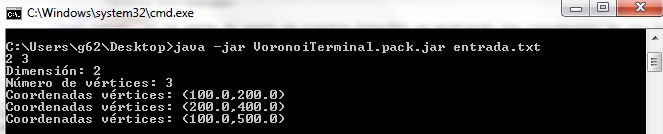
\includegraphics[scale=0.8]{imagenes/terminal1.JPG}
               \caption{Información mostrada en el terminal del fichero de entrada.}
            \end{figure}
        
        \item A continuación, se generará un fichero de texto con extensión .txt ubicado en el mismo directorio donde teníamos el .jar y el fichero de entrada, que mostrará lo siguiente:       
            \begin{figure}[H]
               \centering 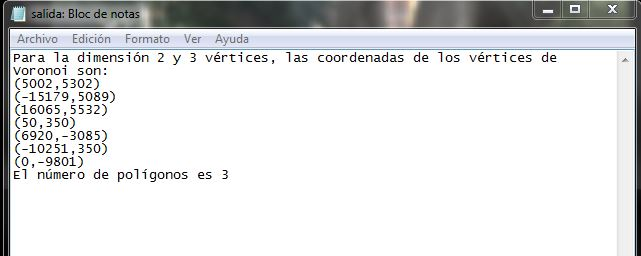
\includegraphics[scale=0.8]{imagenes/terminal2.JPG}
               \caption{Información mostrada en el fichero de salida para dos dimensiones.}
            \end{figure}
            \begin{figure}[H]
               \centering 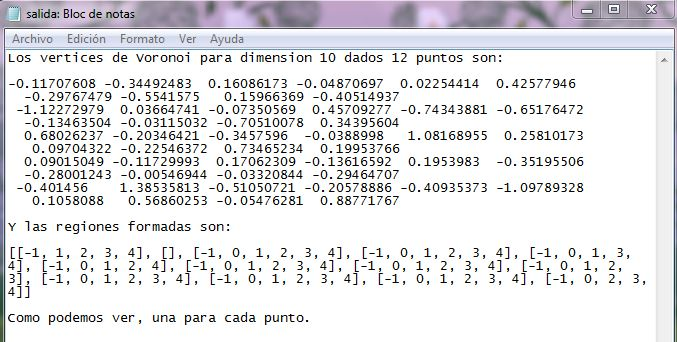
\includegraphics[scale=0.8]{imagenes/terminal13.JPG}
               \caption{Información mostrada en el fichero de salida para diez dimensiones.}
            \end{figure}
    \end{enumerate}

\begin{itemize}
    \item A continuación mostramos el funcionamiento en detalle de la aplicación más completa con interfaz gráfica.
\end{itemize}

\begin{enumerate}
        \item Mostramos la interfaz nada más abrirla: 
        \begin{figure} [H]
            \centering
            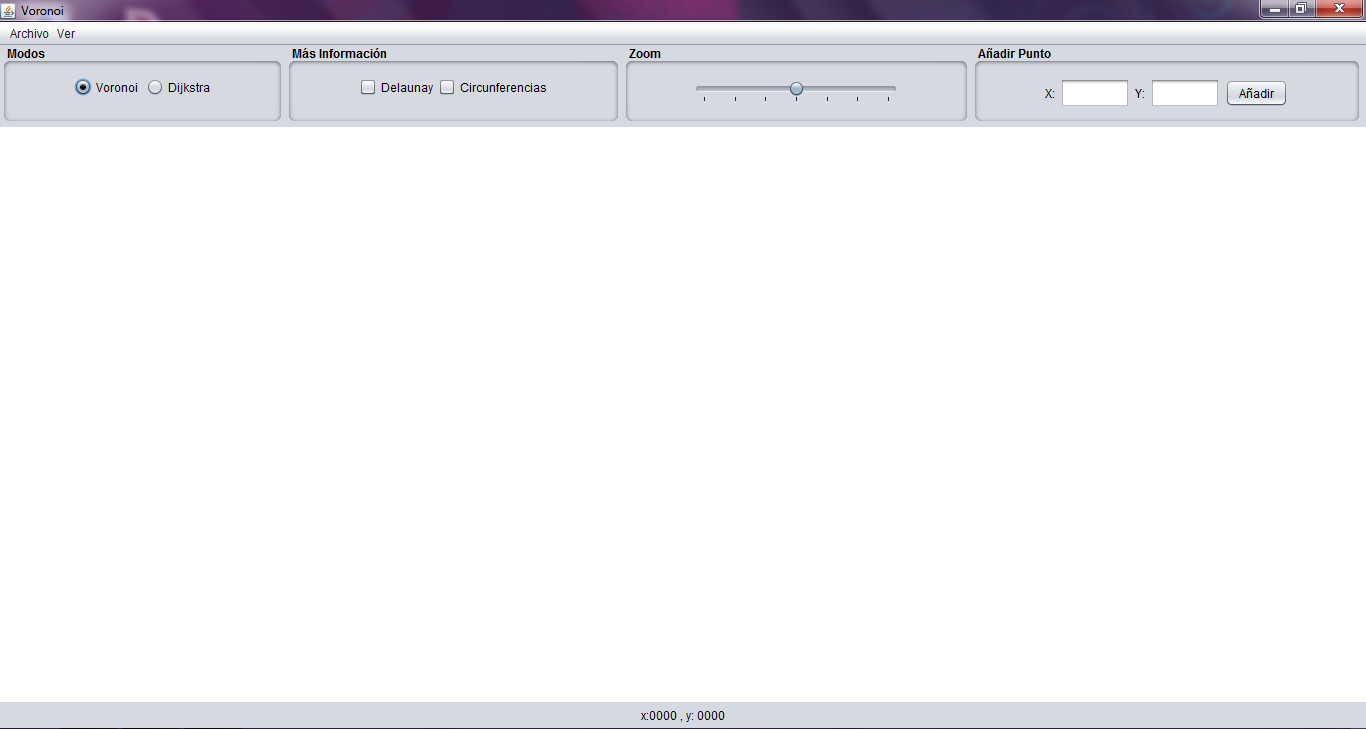
\includegraphics[scale=0.4]{imagenes/inicio.png}
            \caption{Pantalla inicial de la aplicación.}
        \end{figure}
    
        \item En primer lugar, podemos dibujar puntos con el ratón. Por defecto, se nos dibujará el Diagrama de Voronoi ya que éste es el modo inicial, donde cada punto dibujado con el ratón sólo pertenecerá a una región de Voronoi. A continuación se muestra el resultado de 10 puntos dibujados.      
        \begin{figure}  [H]
            \centering
            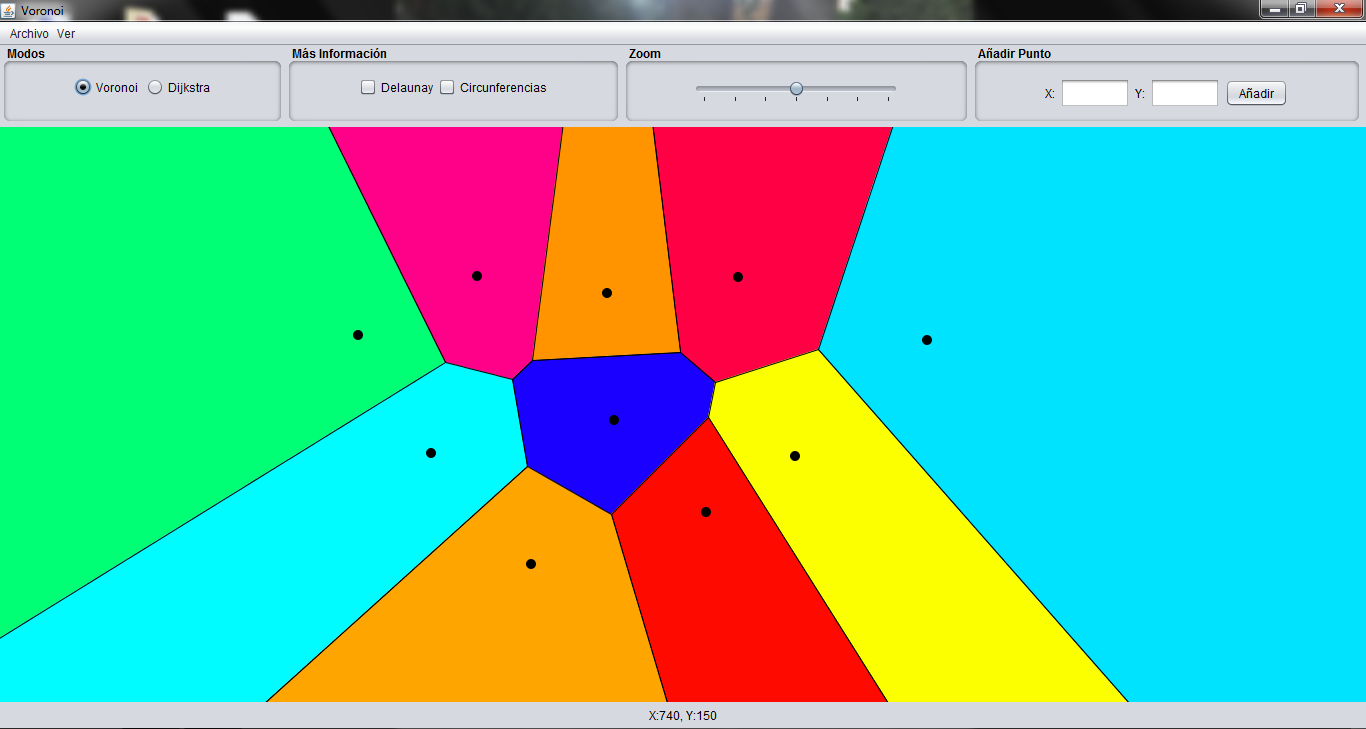
\includegraphics[scale=0.3]{imagenes/voronoi10puntos.png}
            \caption{Diagrama de Voronoi de 10 puntos aleatorios.}
        \end{figure}
                
        \item Si cambiamos el modo a Dijkstra, podremos elegir dos puntos al azar y se nos trazará el camino optimal y más corto posible entre ellos teniendo en cuenta dónde están colocados y evitando acercarse demasiado a los puntos negros. Estos puntos, en nuestra aplicación, serán nuestros atractores por lo que el recorrido de un robot para llegar desde un punto inicial al destino que le indiquemos, deberá alejarse lo máximo posible de ellos. Se calculará trazando perpendiculares desde los puntos seleccionados hasta las aristas de Voronoi para luego moverse por ellas.
        \begin{figure}[H]
            \subfigure[Dijkstra desde dos puntos cualesquiera.]{ 
                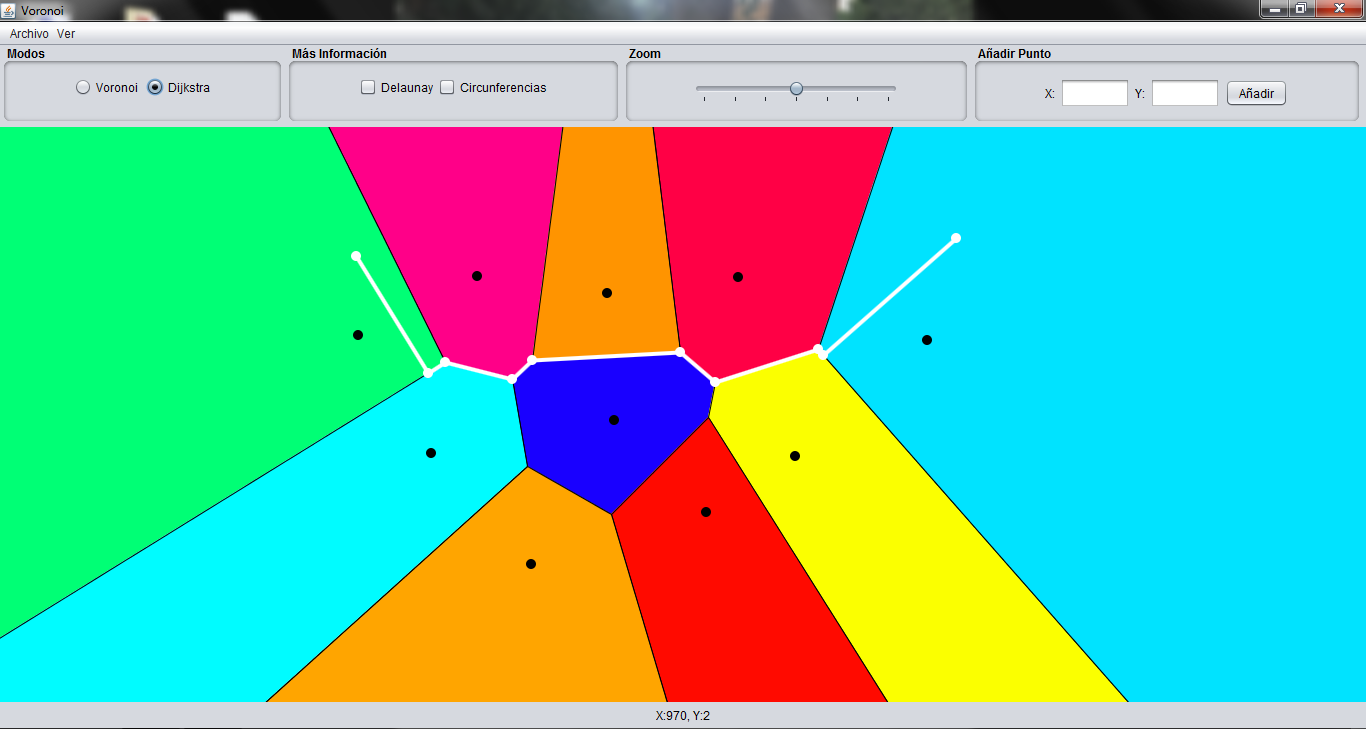
\includegraphics[scale=0.2]{imagenes/dijkstra.png}
            } 
            \subfigure[Dijkstra entre dos puntos que pertenecen a la misma región.]{
                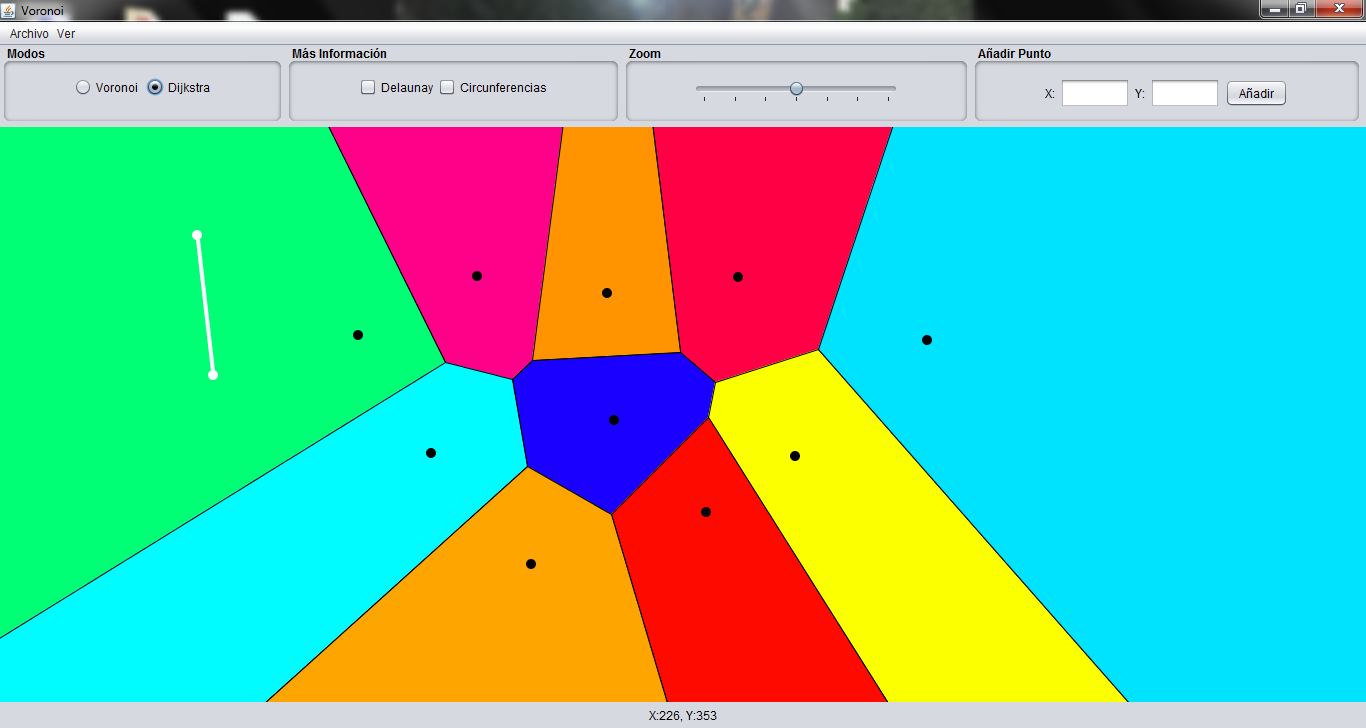
\includegraphics[scale=0.2]{imagenes/dijkstra1.png}
            }
            \subfigure[Dijkstra entre dos puntos que pertenecen a la misma región pero evitando acercarse al atractor.]{
                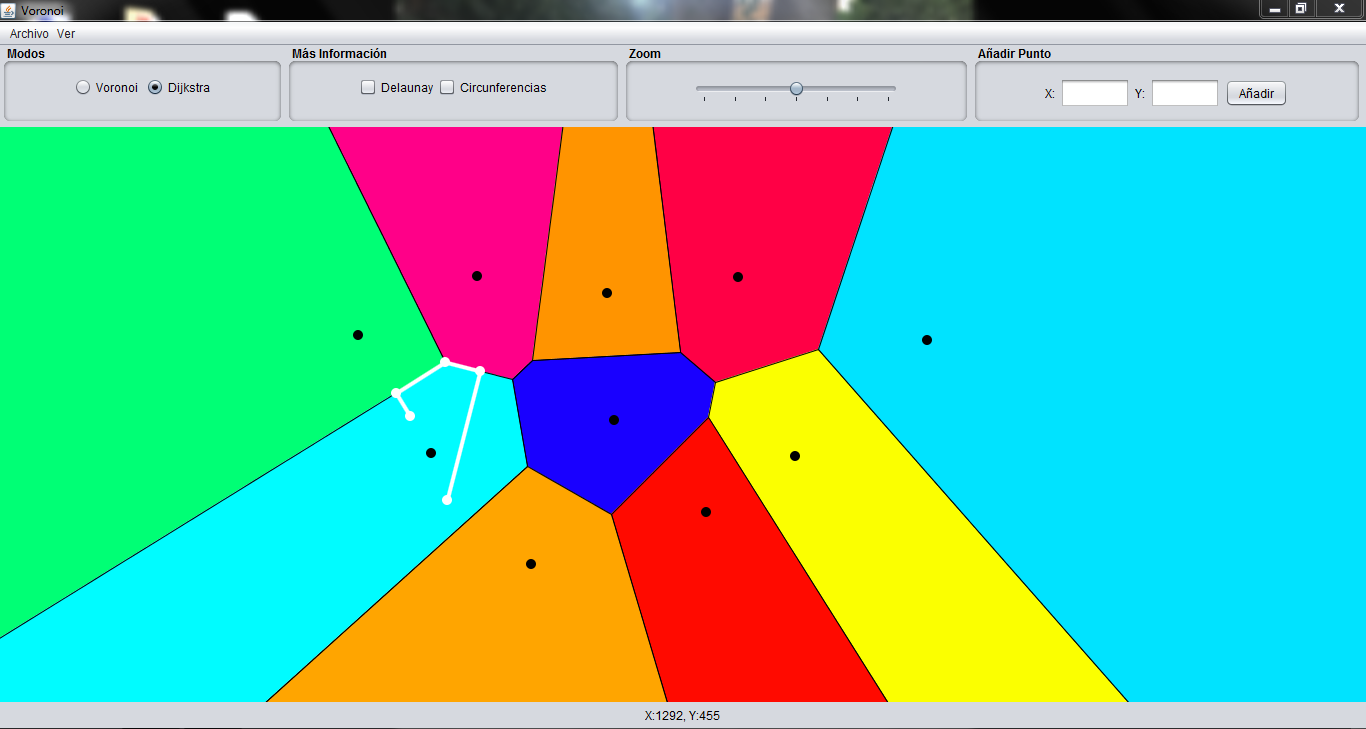
\includegraphics[scale=0.2]{imagenes/dijkstra2.png}
            }
            \subfigure[Dijkstra entre dos puntos pertenecientes a polígonos correlativos.]{ 
                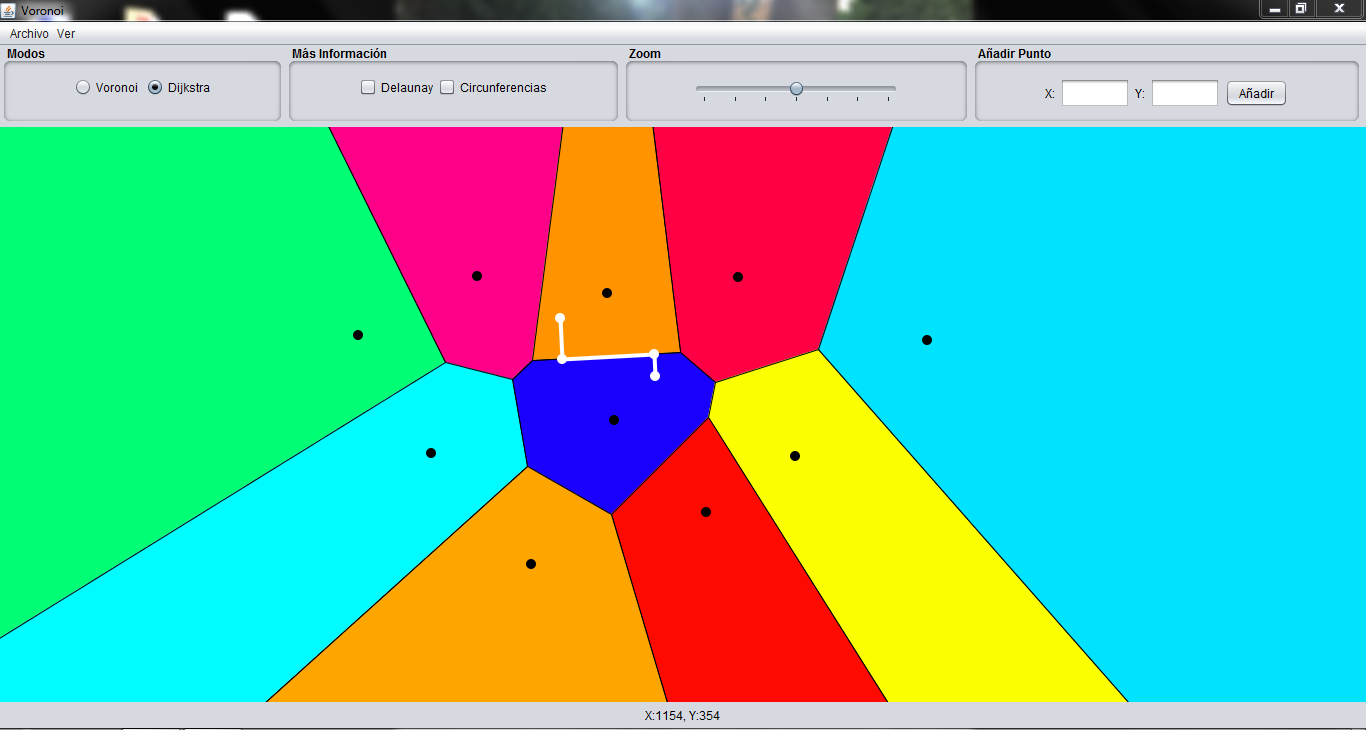
\includegraphics[scale=0.2]{imagenes/dijkstra3.png}
             }            
            \caption{Pruebas del algoritmo de Dijkstra.} \label{fig:incre}
        \end{figure}        
        \item Además, ofrecemos más información: Si seleccionamos ``Delaunay", se dibujará la correspondiente Triangulación de Delaunay.   
        \begin{figure}  [H]
            \centering
            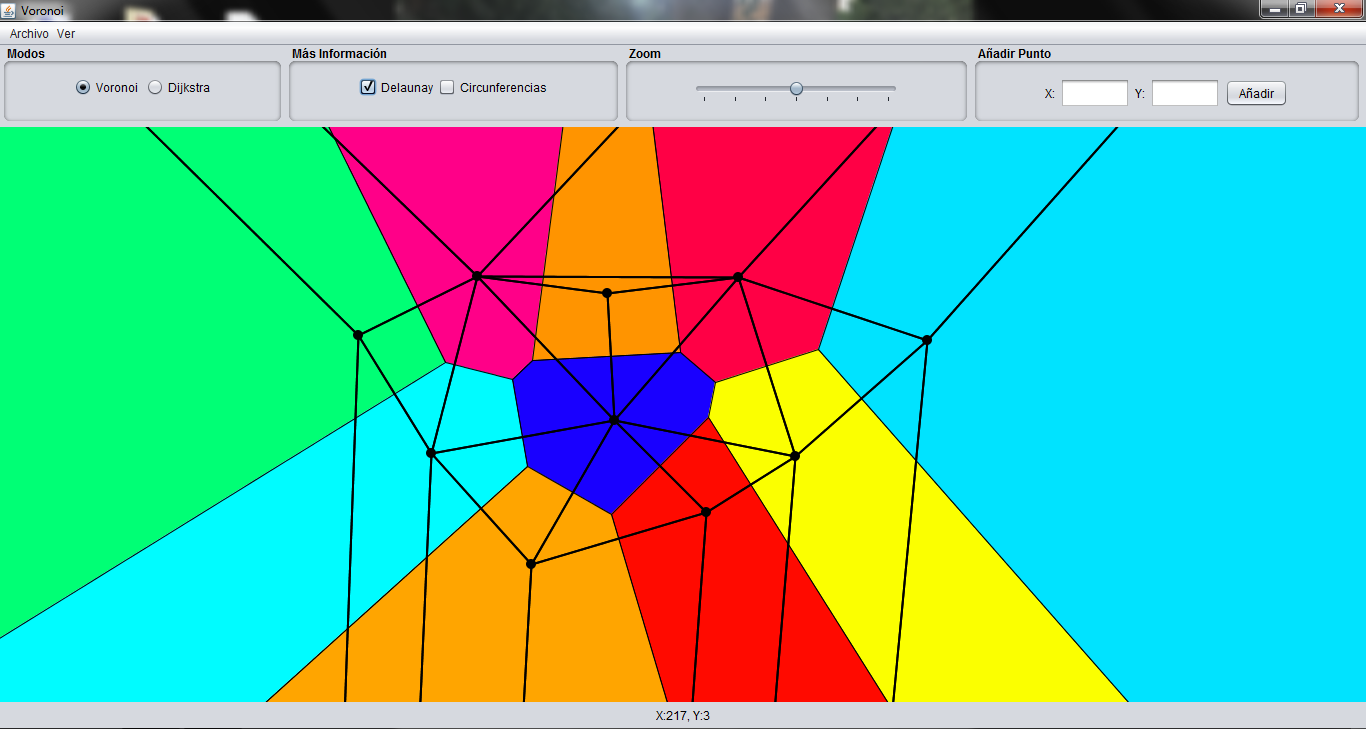
\includegraphics[scale=0.3]{imagenes/delaunay.png}
            \caption{Triangulación de Delaunay del Diagrama de Voronoi dibujado anteriormente con 10 puntos aleatorios.}
        \end{figure}
        
        \item Otra información que podemos mostrar es, al seleccionar ``Circunferencias", se dibujará la correspondiente Triangulación de Delaunay.   
        \begin{figure}  [H]
            \centering
            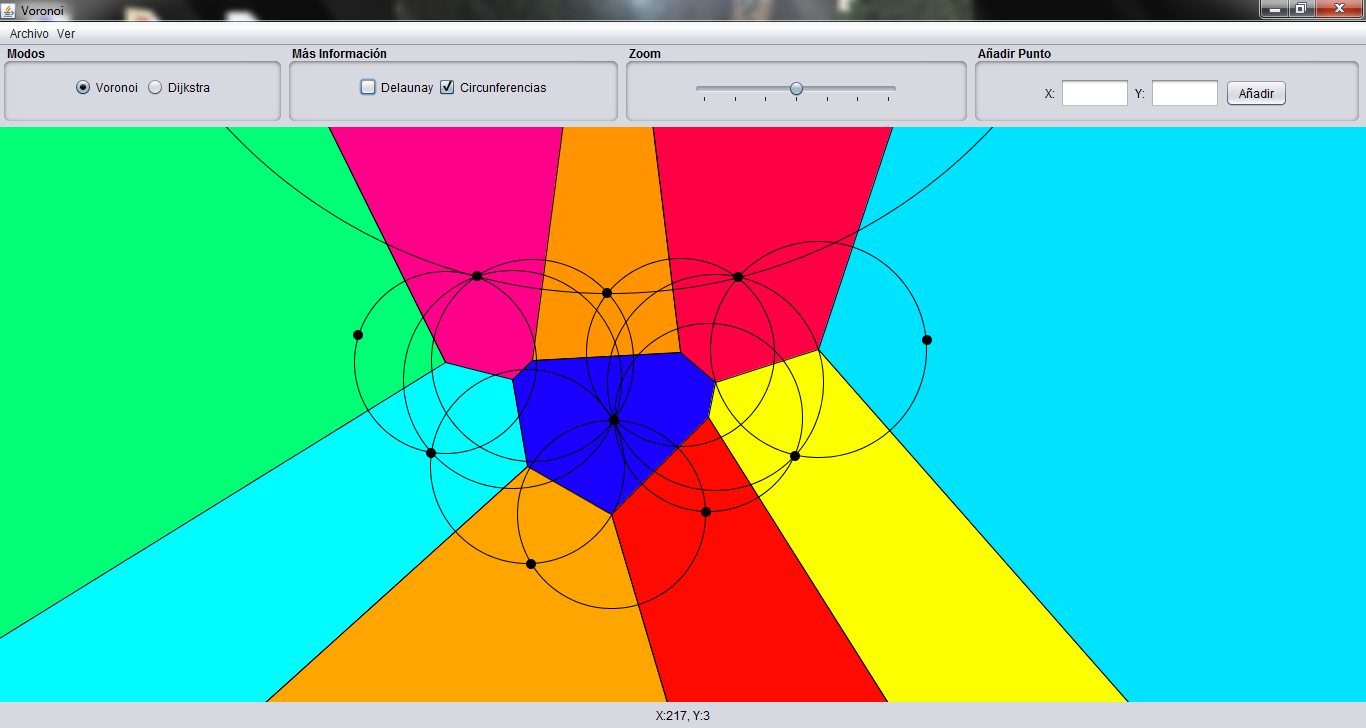
\includegraphics[scale=0.3]{imagenes/circunferencias.png}
            \caption{Circunferencias circunscritas de la Triangulación de Delaunay.}
        \end{figure}
             
        \item Podemos además darle y quitarle zoom a lo dibujado moviendo la barra de desplazamiento, y se nos permitirá seguir dibujando siempre que lo deseemos.        
         \begin{figure}[H]
            \subfigure[Damos zoom.]{ 
                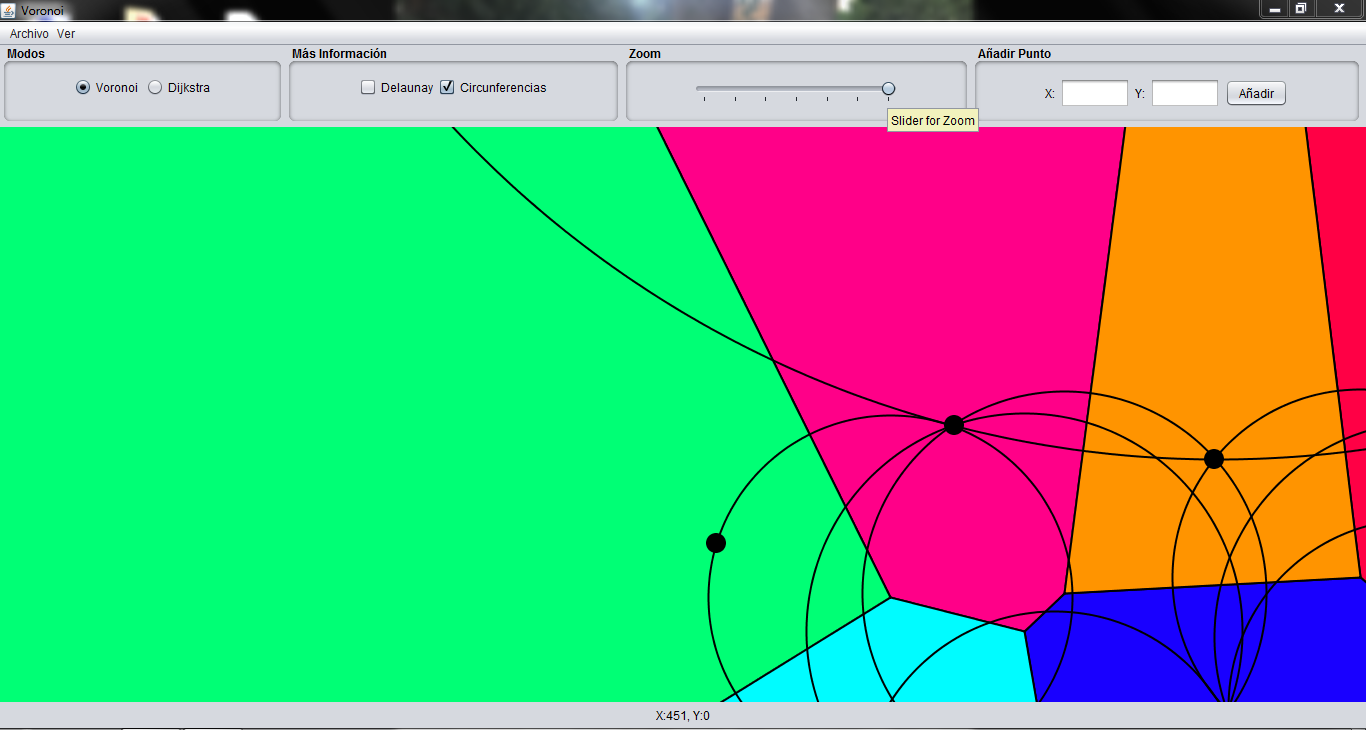
\includegraphics[scale=0.2]{imagenes/maszoom.png}
             } 
            \subfigure[Quitamos zoom.]{
                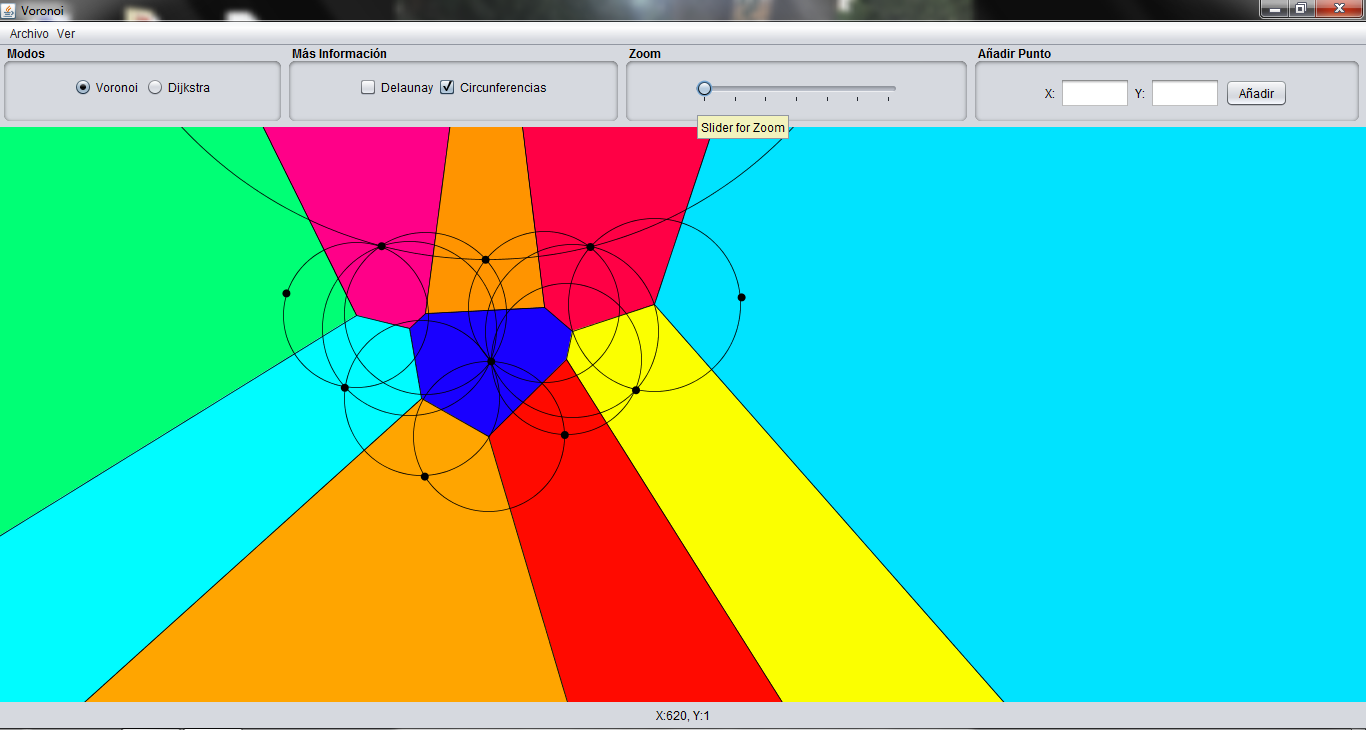
\includegraphics[scale=0.2]{imagenes/menoszoom.png}
            }                       
            \caption{Hacemos zoom en la barra de desplazamiento de la parte superior de nuestra aplicación.} \label{fig:incre}
        \end{figure}
        
         \item Podemos añadir puntos indicando sus coordenadas X e Y. Por ejemplo, añadimos a continuación el punto $(100,200)$.    
         \begin{figure}[H]
            \subfigure[Indicamos las coordenadas del punto.]{ 
                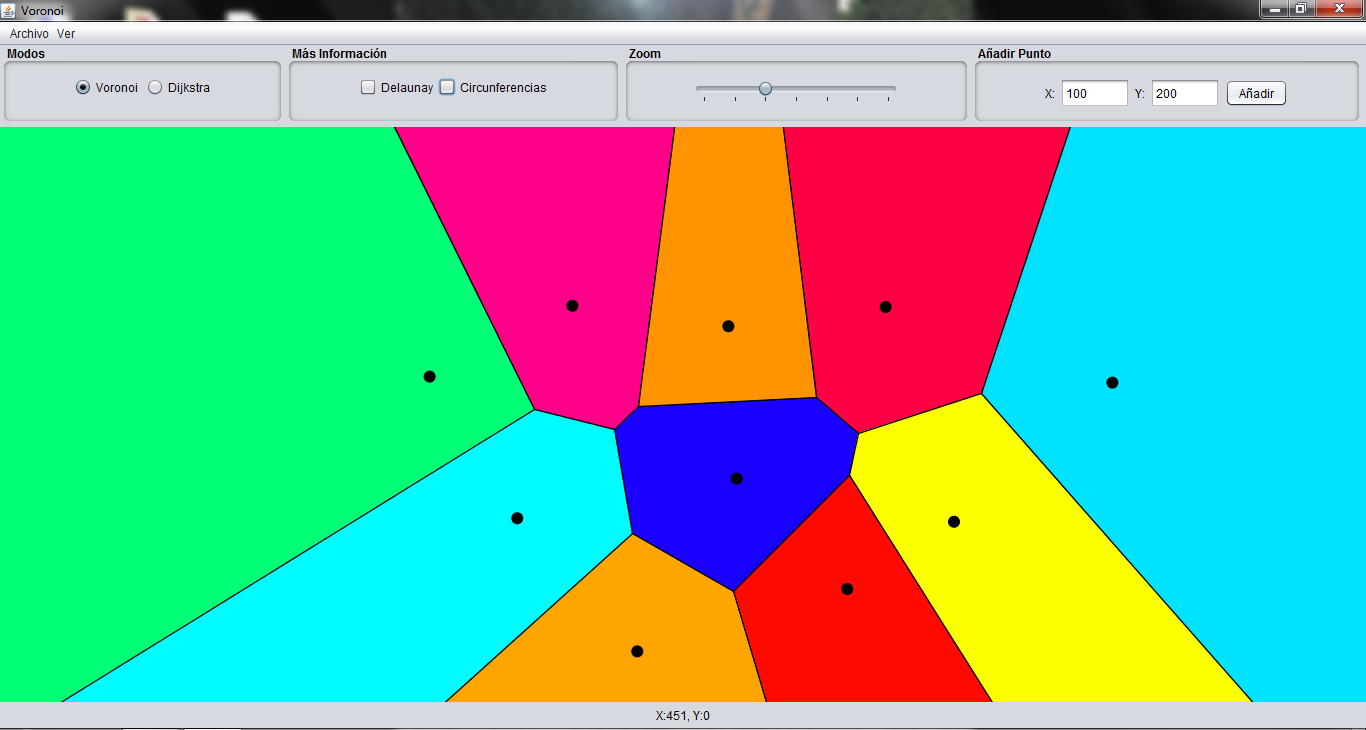
\includegraphics[scale=0.2]{imagenes/aniadimospunto.png}
             } 
            \subfigure[Vemos el punto que acabamos de introducir, en la región morada.]{
                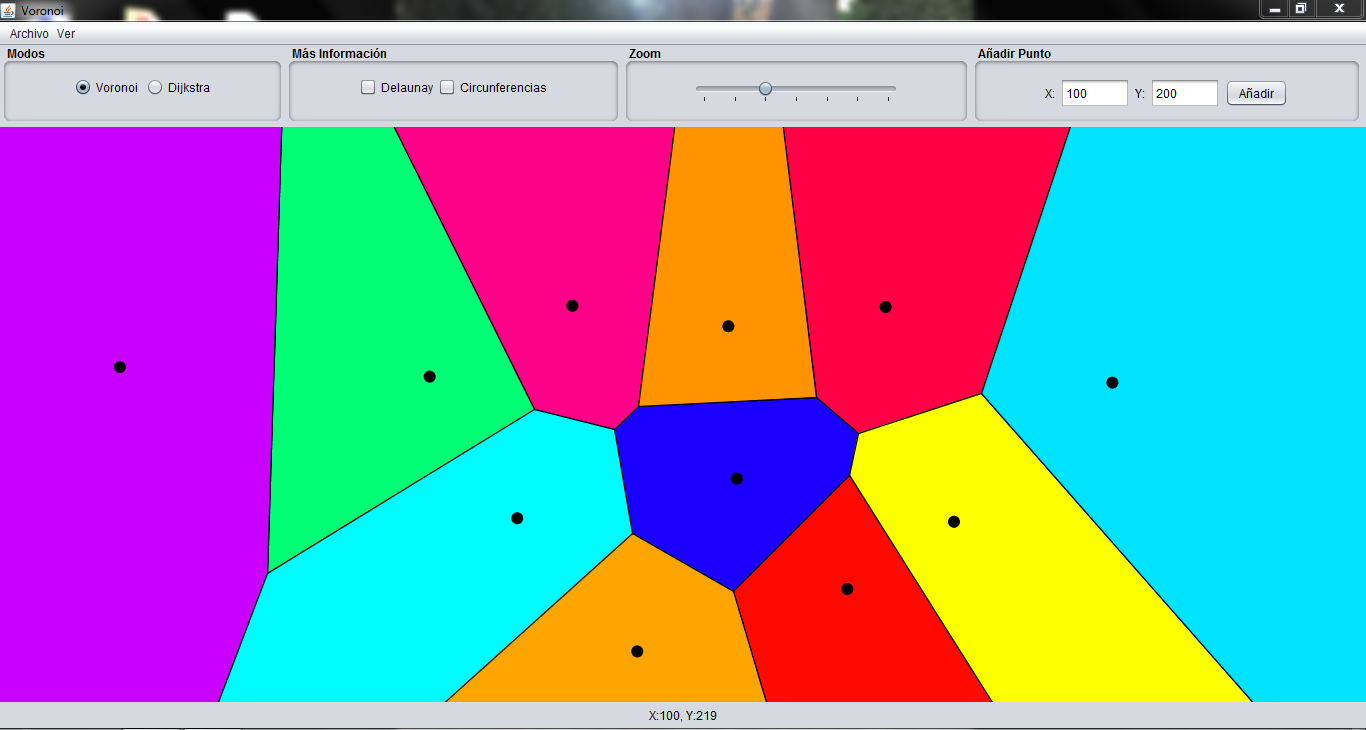
\includegraphics[scale=0.2]{imagenes/aniadimospunto1.png}
            }                       
            \caption{Añadimos un punto indicando sus coordenadas en la parte superior derecha de la aplicación.} \label{fig:incre}
        \end{figure}
        
        \item Podemos añadir o quitar la barra de herramientas en la opción ``Ver" del menú arriba a la izquierda:
        \begin{figure}[H]
            \centering
            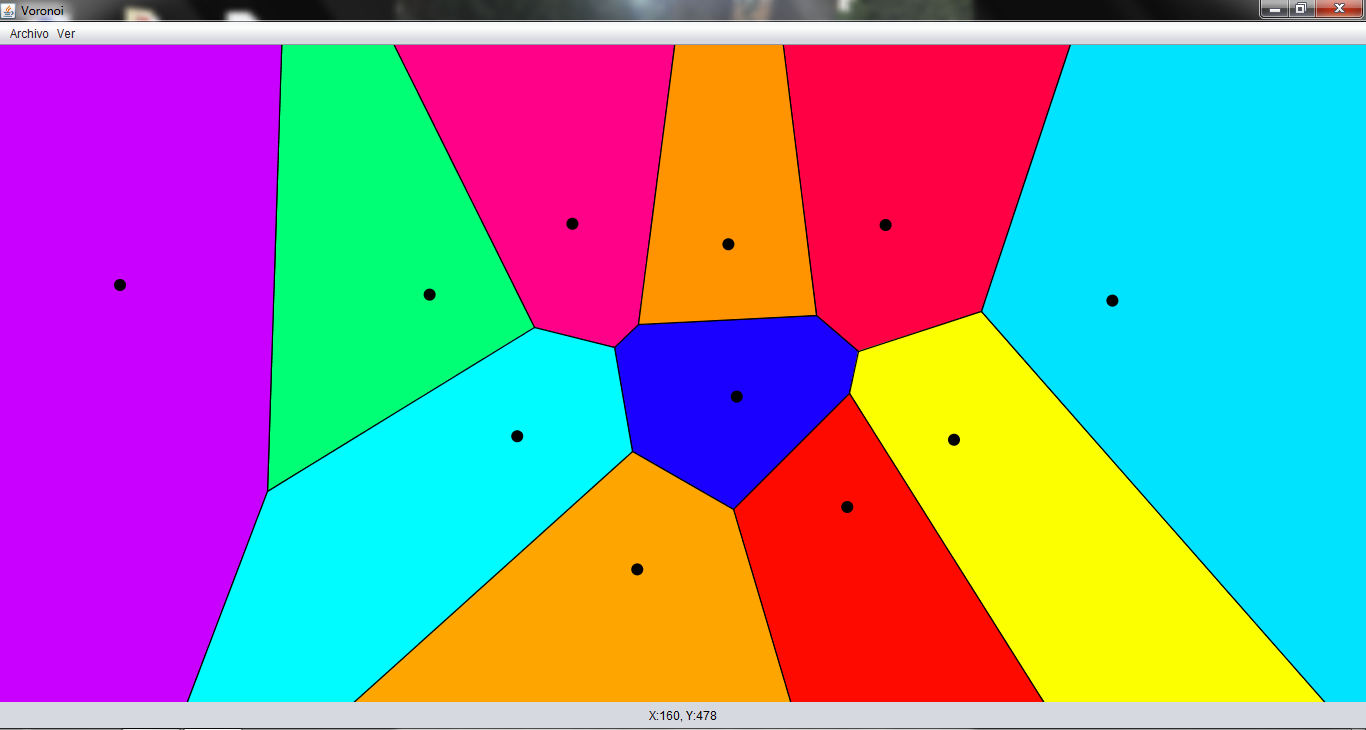
\includegraphics[scale=0.3]{imagenes/nobarraherramientas.png}
            \caption{Aplicación sin la barra de herramientas superior.}
        \end{figure}        
        \item Para trabajar con archivos tenemos diferentes opciones pulsando en ``Archivo" del menú superior izquierdo de nuestra aplicación:
        \begin{enumerate}
            \item Guardar archivo: guardaremos el dibujo actual en un archivo con extensión \textit{.txt}.
            \begin{figure}[H]
                \subfigure[Pulsamos la opción de Guardar.]{             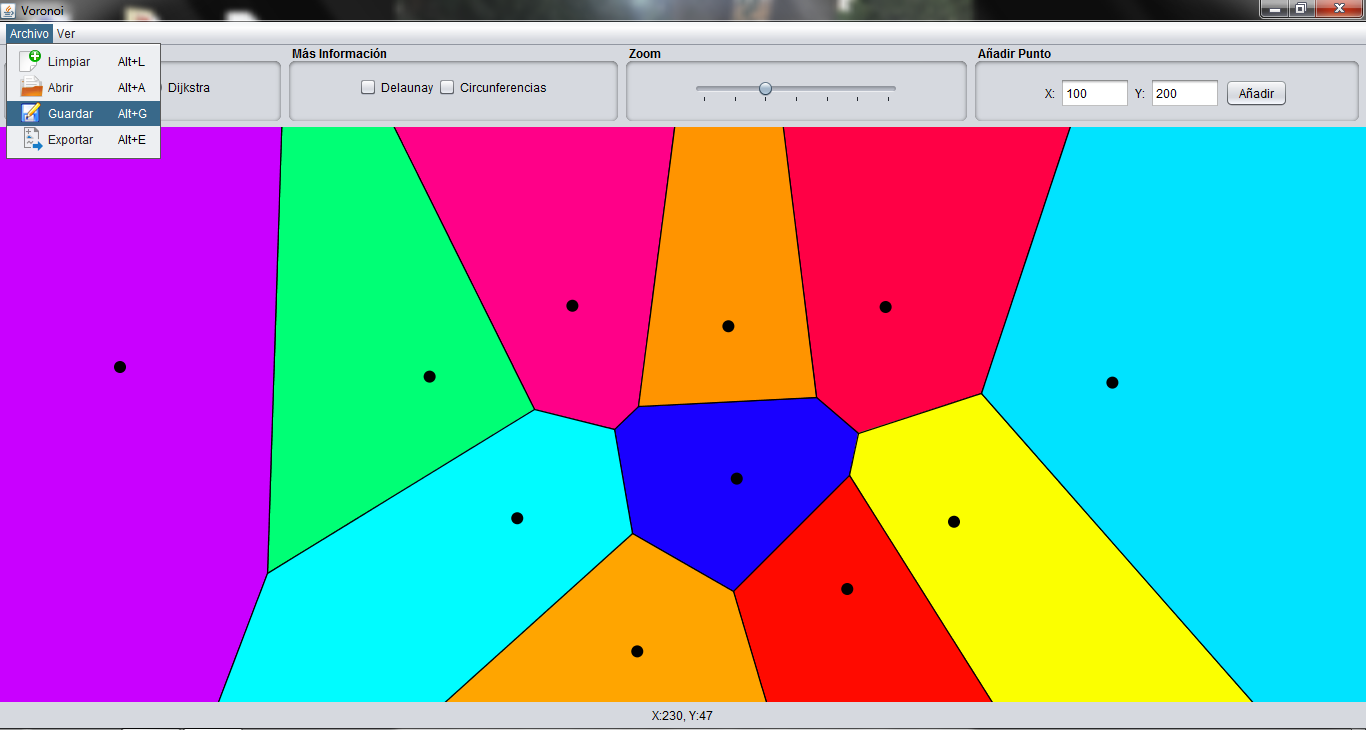
\includegraphics[scale=0.2]{imagenes/guardar.png}
                 } 
                \subfigure[Le damos nombre al archivo que queremos guardar.]{                   \includegraphics[scale=0.2]{imagenes/guardar1.png}
                }                    
                \begin{center}
                \subfigure[El archivo guardado contiene esta información: dimensión, número de vértices y coordenadas de los vértices.]{                  
                \includegraphics[scale=1]{imagenes/guardar2.JPG}
                    
                }\end{center}               
                \caption{Guardar archivo.} \label{fig:incre}
            \end{figure}
        
            \item Exportar archivo: guardaremos el dibujo actual en un archivo con extensión \textit{.txt} con los datos necesarios para que cualquier persona pueda representar nuestro Diagrama de Voronoi:            
            \begin{figure}[H]
                \subfigure[Pulsamos la opción de Exportar.]{               \includegraphics[scale=0.2]{imagenes/exportar.png}
                 } 
                \subfigure[Le damos nombre al archivo que queremos exportar.]{                  \includegraphics[scale=0.2]{imagenes/exportar1.png}
                }                    
                \begin{center}
                \subfigure[El archivo exportado contiene esta información: lista de vértices de Voronoi y si están conectados o no (indicándolo con 0 y 1 respectivamente).]{          \includegraphics[scale=0.8]{imagenes/exportar2.JPG}                   
                }\end{center}               
                \caption{Exportar archivo.} \label{fig:incre}
            \end{figure}
            
            \item Limpiar: esta opción nos pone la pantalla en blanco, tal y como la encontramos al principio del todo.           
             \begin{figure}[H]
                \subfigure[Pulsamos la opción de Limpiar.]{                \includegraphics[scale=0.18]{imagenes/limpiar.png}
                } 
                \subfigure[Aplicación lista para empezar de nuevo.]{  \includegraphics[scale=0.18]{imagenes/limpiar1.png}
                }                            
                \caption{Exportar archivo.} \label{fig:incre}
                
            \end{figure} 
            
            \item Abrir archivo: podemos abrir un archivo que tendrá los datos necesarios para poder representarlo en nuestra aplicación, es decir: dimensión, número de vértices y coordenadas de los vértices. Lo probamos para el archivo anteriormente guardado, por lo que nos saldrá el mismo dibujo con colores diferentes ya que éstos se seleccionan de manera aleatoria: 
            \begin{figure}[H]
                \begin{center}               
               \subfigure[Pulsamos la opción de Abrir.]{                   \includegraphics[scale=0.3]{imagenes/abrir.png}
                 } 
                \subfigure[Elegimos el archivo que queremos abrir.]{ \includegraphics[scale=0.3]{imagenes/abrir1.png}
                }     
                \subfigure[Se muestra el archivo seleccionado.]{    \includegraphics[scale=0.3]{imagenes/abierto.png}
                } 
                 \end{center}
                \caption{Abrir archivo.} \label{fig:incre}
            \end{figure}                  
        \end{enumerate}             
        
        \item Además, podemos mostrar varia información a la vez.
        \begin{figure}  [H]
            \centering
            \includegraphics[scale=0.3]{imagenes/todo.png}
            \caption{Mostramos información completa.}
        \end{figure}
    \end{enumerate}
    

\section{Código desarrollado} \label{manual}

El código elaborado en dos proyectos de Java, uno para la aplicación desde terminal (en la carpeta \textit{VoronoiTerminal}) y otro para la interfaz gráfica (dentro de la carpeta \textit{VoronoiDijkstraApp}) así como la librería implementada (\textit{Voronoi.MOB.Biblioteca}), puede encontrarse en el siguiente enlace:
\hspace{0.3cm}

\begin{center} 
\url{https://github.com/MariaOB/TFG}
\end{center}

\hspace{0.3cm}
Dentro de la carpeta \textit{dist} de los directorios donde se encuentran ambas aplicaciones, podemos obtener los .jar que comentábamos anteriormente donde se pueden ejecutar las aplicaciones teniendo Java instalado en nuestra computadora.